%%
\documentclass[12pt,a4paper,english,greek,twoside]{ceid-thesis}
\usepackage{graphicx}
\usepackage{epstopdf}
\usepackage{indentfirst}
\usepackage{verbatim}
\usepackage{amsmath}
\usepackage{amsthm}
\usepackage{amssymb}
\usepackage{gensymb}
\usepackage{latexsym}
\bibliographystyle{static/hellas}
\usepackage{hyphenat}
\usepackage{makeidx}
\usepackage{tabularx}
\usepackage{epigraph}
\usepackage{caption}
\usepackage{textcomp}
\usepackage[utf8]{inputenc}

%\usepackage{titlesec}
%\setcounter{secnumdepth}{4}

\usepackage{listings}
\usepackage{color}

\usepackage{xcolor}
\usepackage{colortbl}

\definecolor{blizzardblue}{rgb}{0.67, 0.9, 0.93}
\definecolor{classicrose}{rgb}{0.98, 0.8, 0.91}

\definecolor{codegreen}{rgb}{0,0.6,0}
\definecolor{codegray}{rgb}{0.5,0.5,0.5}
\definecolor{light-gray}{gray}{0.95}
\definecolor{codepurple}{rgb}{0.58,0,0.82}
\definecolor{backcolour}{rgb}{0.95,0.95,0.92}

\lstdefinestyle{mystyle}{
    %backgroundcolor=\color{backcolour},
    backgroundcolor=\color{light-gray},
    commentstyle=\color{codegreen},
    keywordstyle=\color{magenta},
    numberstyle=\tiny\color{codegray},
    stringstyle=\color{codepurple},
    basicstyle=\footnotesize,
    %basicstyle=\ttfamily\footnotesize,
    breakatwhitespace=false,         
    breaklines=true,                 
    captionpos=b,                    
    keepspaces=true,                 
    numbers=left,                    
    numbersep=5pt,                  
    showspaces=false,                
    showstringspaces=false,
    showtabs=false,                  
    tabsize=2
}

\usepackage{algorithm}
\usepackage{algorithmic}
\makeatletter
\renewcommand{\ALG@name}{{\en {Algorithm}}}
\renewcommand{\listalgorithmname}{List of \ALG@name s}
\makeatother

\lstset{style=mystyle}

\useshorthands{;}
\defineshorthand{;}{?}
\addto\captionsgreek{%
  \renewcommand{\indexname}{Ευρετήριο όρων}%
}
\makeindex

% \epigraphsize{\small}% Default
\setlength\epigraphwidth{15cm}
\setlength\epigraphrule{0pt}

\usepackage{etoolbox}

\makeatletter
\patchcmd{\epigraph}{\@epitext{#1}}{\itshape\@epitext{#1}}{}{}
\makeatother

% 1.5 spacing
\renewcommand{\baselinestretch}{1.2}

% latin text (and greek text)
\newcommand{\tl}[1]{\textlatin{#1}}
\newcommand{\tg}[1]{\textgreek{#1}}

% typeset short english phrases
\newcommand{\en}[1]{\foreignlanguage{english}{#1}}

% typeset source code
\newcommand{\src}[1]{{\tt\en{#1}}}

% typeset a backslash
\newcommand{\bkslash}{\en{\symbol{92}}}

\newtheorem{definition}{Ορισμός}
\newtheorem{proposition}{Πρόταση}
\newtheorem{theorem}{Θεώρημα}
\newtheorem{corollary}{Συμπέρασμα}
\newtheorem{lemma}{Λήμμα}
\newtheorem{example}{Παράδειγμα}
\newtheorem{remark}{Σημείωση}
\newtheorem{notation}{Συμβολισμός}
\newtheorem{law}{Νόμος}
\renewcommand{\thedefinition}{\arabic{chapter}.\arabic{definition}}
\renewcommand{\theproposition}{\arabic{chapter}.\arabic{proposition}}
\renewcommand{\thetheorem}{\arabic{chapter}.\arabic{theorem}}
\renewcommand{\thecorollary}{\arabic{chapter}.\arabic{corollary}}
\renewcommand{\thelemma}{\arabic{chapter}.\arabic{lemma}}
\renewcommand{\theexample}{\arabic{chapter}.\arabic{example}}
\newcommand{\set}[1]{\left\{#1\right\}}
\newcommand{\To}{\Longrightarrow}
\newcommand{\xml}{\en{XML}}

\selectlanguage{greek}

\hyphenation{ο-ποί-α}

%%%%%%%%%%%%%%%%%%%%%%%%%%%%%%%%%%%%%%%%%%%%%%%%%%%%%
%% THESIS INFO 
%%
%
% Τίτλος Πτυχιακής Εργασίας
	\title{Σύστημα Επεξεργασίας, \\ Ανάλυσης και Ομαδοποίησης \\ Εγγράφων Ειδήσεων του Διαδικτύου}
% "του" ή "της", ανάλογα με το φύλο του σπουδαστή
	\edef\toutis{της}
% Ονοματεπώνυμο σπουδαστή (ΚΕΦΑΛΑΙΑ, γενική πτώση)
	\edef\authorNameCapital{ΑΦΡΟΔΙΤΗΣ ΑΛΕΒΙΖΟΠΟΥΛΟΥ}
% Ονοματεπώνυμο σπουδαστή (πεζά, ονομαστική πτώση)
	\author{Αφροδίτη Αλεβιζοπούλου}
% Ονοματεπώνυμο Επιβλέποντα Καθηγητή
	\supervisor{Ιωάννης Χατζηλυγερούδης}
    \edef\supervisorTitle{Καθηγητής}
% Ονοματεπώνυμο Επιβλέποντα Καθηγητή
	\supervisorSecond{}
    \edef\supervisorSecondTitle{ Τίτλος}
% "Επιβλέπων" ή "Επιβλέπουσα", ανάλογα με το φύλο του Επιβλέποντα Καθηγητή
	\edef\supervisorMaleFemale{Επιβλέπων}
% Τόπος, μήνας και έτος
	\edef\thesisPlaceDate{Πάτρα, Νοέμβριος 2017}
% Ημερομηνία Εξέτασης % 19η Δεκεμβρίου 2016
	\edef\examinationDate{16η Νοεμβρίου 2017}
% Έτος Copyright
	\edef\copyrightYear{2017}
% Ονοματεπώνυμο 1ου εξεταστή
	\epitropiF{ }
% Τίτλος 1ου εξεταστή
	\edef\epitropiFTitle{ }
% Ονοματεπώνυμο 2ου εξεταστή
	\epitropiS{ }
% τίτλος 2ου εξεταστή
	\edef\epitropiSTitle{}
%%%%%%%%%%%%%%%%%%%%%%%%%%%%%%%%%%%%%%%%%%%%%%%%%%%%%


\begin{document}
\selectlanguage{greek}
\maketitle

\frontmatter
% Ευχαριστίες
	\begin{acknowledgements}
Στο σημείο αυτό είναι απαραίτητο να ευχαριστήσω όλους όσους συνέβαλλαν 
στην εκπόνηση και συγγραφή της διπλωματικής μου εργασίας. 
\par Ευχαριστώ θερμά τον Καθηγητή κ. Ιωάννη Χατζηλυγερούδη για την εμπιστοσύνη που μου έδειξε 
αναθέτοντάς μου την εκπόνηση της συγκεκριμένης διπλωματικής. 
\par Θα ήθελα επίσης να ευχαριστήσω τον επιβλέποντα της διπλωματικής μου εργασίας, Διδάκτορα κ. Ισίδωρο Περίκο, 
για τη συνεχή καθοδήγησή του, τις χρήσιμες συμβουλές του, αλλά και την εξαιρετική
συνεργασία που είχαμε. 
\par Τέλος, ευχαριστώ την οικογένειά μου και τον αγαπημένο μου φίλο, Αλέξανδρο Αντωνόπουλο, 
για τη στήριξη και την καθοδήγηση που μου προσέφεραν καθ'όλη τη διάρκεια των σπουδών μου.
\end{acknowledgements}
	% Αφιέρωση
	\thesisDedication{Στη μνήμη της μητέρας μου, Χριστίνας-Λώρεν Αλεβιζοπούλου \\
	και του αγαπημένου δασκάλου και φίλου, Νώντα Καρύμπαλη}
% Περίληψη
	\begin{abstract}

Λόγω του μεγάλου όγκου πληροφοριών που κατακλύζει το διαδίκτυο, συχνά οι χρήστες
δυσκολεύονται να ξεχωρίσουν τις πληροφορίες που πραγματικά σχετίζονται με τα
ενδιαφέροντά τους. Επιπλέον, οι χρήστες έχουν πολύ διαφορετικά ενδιαφέροντα ή
προτιμήσεις που μπορούν να ληφθούν υπόψη ώστε να φιλτραριστούν ή να
ταξινομηθούν τα αποτελέσματα μιας ερώτησης με σκοπό το αποτέλεσμα να ικανοποιεί
τις εξατομικευμένες ανάγκες κάθε χρήστη. Η κατηγορία αυτών των συστημάτων
εξατομίκευσης ονομάζεται “Συστήματα Συστάσεων” {\en {(Recommender Systems)}}. Τα
Συστήματα Συστάσεων εκμεταλλεύονται τις ιδιαιτερότητες των χρηστών με σκοπό να τους 
διευκολύνουν στο να προσδιορίζουν ακριβέστερα τις πληροφορίες ή τις υπηρεσίες για
τις οποίες ενδιαφέρονται περισσότερο ή σχετίζονται με τις ανάγκες τους, κάνοντας
χρήση ειδικών αλγορίθμων. Οι αλγόριθμοι που χρησιμοποιούνται λαμβάνουν ως
είσοδο τα χαρακτηριστικά και τις προτιμήσεις των χρηστών ή τις σχέσεις μεταξύ των
χρηστών ή τα γνωρίσματα των προς σύσταση αντικειμένων και υπολογίζουν το
εκτιμώμενο ενδιαφέρον του χρήστη για κάθε αντικείμενο. Στην συνέχεια ταξινομούν ή
φιλτράρουν τα αντικείμενα με κριτήριο το εκτιμώμενο ενδιαφέρον. \\

Στο πλαίσιο της παρούσας διπλωματικής εργασίας σχεδιάστηκε και υλοποιήθηκε ένα 
σύστημα επεξεργασίας, ανάλυσης και ομαδοποίησης εγγράφων ειδήσεων του διαδικτύου, 
σχεδιασμένο ως εφαρμογή ειδησεογραφικού περιεχομένου που επιτρέπει στο χρήστη 
την περιήγηση μεταξύ των άρθρων μιας βάσης δεδομένων 
και λαμβάνοντας υπόψη τις επιλογές του, δηλαδή το προφίλ/ιστορικό του κάθε χρήστη, 
του προτείνει νέα άρθρα ειδήσεων που ταιριάζουν περισσότερο με τα ενδιαφέροντά του 
και δίνει τη δυνατότητα παρουσίασης των ειδήσεων οι οποίες σχετίζονται σημασιολογικά με αυτές που
έχει ήδη αναγνώσει.

\begin{keywords}
%\tl{RDF/S}, \tl{RQL}, \tl{Jxta}
\textit{Μηχανική Εκμάθηση, 
   %Συστήματα Συστάσεων, 
   Πολυεπίπεδο Σύστημα Συστάσεων Διαδικτυακών Εγγράφων Ειδήσεων, 
   Προσωποποιημένη Ανάκτηση Περιεχομένου, 
   Προσωποποιημένα Διαδικτυακά Έγγραφα Ειδήσεων, 
   Εξατομίκευση, Προφίλ Χρήστη, Μοντέλα Θεμάτων}
\end{keywords}
\end{abstract}


% Πίνακας Περιεχομένων
	\tableofcontents
% Κατάλογος Σχημάτων
	%\listoffigures
% Κατάλογος Πινάκων
	%\listoftables

%%%%%%%%%%%%%%%%%%%%%%%%%%%%%%%%%%%%%%%%%%%%%%%%%%%%%
%% INCLUDE YOUR CHAPTERS/SECTIONS HERE
%%
\mainmatter
% Εισαγωγή
	\chapter{Εισαγωγή}

Η ραγδαία εξέλιξη του Παγκόσμιου Ιστού τα τελευταία χρόνια κατέστησε το διαδίκτυο
προσβάσιμο σε εκατομμύρια χρήστες, επιτρέποντας με αυτό τον τρόπο όχι μόνο να
έχουν πρόσβαση σε περισσότερη πληροφορία παγκόσμιων ειδήσεων, αλλά να μπορούν
να ενημερώνονται και πιο γρήγορα. 
Υπάρχουν αρκετοί παράγοντες που συνετέλεσαν στην επιτυχία αυτή του
διαδικτύου, όπως, για παράδειγμα, το μειωμένο κόστος της διανομής και της
πρόσβασης στις ειδήσεις, η διαθεσιμότητα του διαδικτύου σε μια πληθώρα από
πλατφόρμες περιηγητών, η παγκόσμια αποστολή και κατανάλωση πληροφορίας, ο
μικρός χρόνος για τη δημοσίευση ειδήσεων κλπ. 

\par Λόγω της μεγάλης ποσότητας ειδήσεων που δημοσιεύονται κάθε μέρα, 
είναι δύσκολο να βρει κανείς νέες ειδήσεις που τον ενδιαφέρουν. 
Μια λύση σε αυτό το πρόβλημα είναι τα “Συστήματα Συστάσεων” {\en {(Recommender Systems)}}, 
τα οποία χρησιμοποιούν αλγόριθμους συσχέτισης, οι οποίοι, με βάση διαφόρων ειδών
πληροφορίες για τους χρήστες, επιλέγουν και προτείνουν σε αυτούς συγκεκριμένα
προϊόντα ή υπηρεσίες, ανάλογα με τις προτιμήσεις τους.

\newpage

\section{Σκοπός και Διάρθρωση της Διπλωματικής Εργασίας}
% Κλιμακωτό δύο-επιπέδων Σύστημα Συστάσεων Διαδικτυακών Εγγράφων Ειδήσεων
Η παρούσα διπλωματική εργασία επικεντρώνεται στο πεδίο των Συστημάτων Συστάσεων
και στο πλαίσιό της σχεδιάστηκε και υλοποιήθηκε
ένα σύστημα συστάσεων ειδησεογραφικού περιεχομένου που προτείνει άρθρα ειδήσεων σε μεμονωμένους χρήστες. \\

Η εργασία είναι οργανωμένη σε έξι κεφάλαια: \\

\par Στο κεφάλαιο 1 παρουσιάζονται κάποιες θεωρητικές έννοιες που σχετίζονται με την Τεχνητή Νοημοσύνη (ΤΝ), 
εισάγεται ο ορισμός της ΤΝ όπως έχει διαμορφωθεί μέχρι σήμερα και εξηγείται λεπτομερώς τι είναι η ΤΝ. 
Στη συνέχεια, δίνονται ιστορικά στοιχεία που αφορούν στη δημιουργία και εξέλιξή της μέσα στο χρόνο, 
καθώς, επίσης, αναλύονται τομείς στους οποίους αυτή χρησιμοποιείται, 
δίνοντας έμφαση στο πώς έχει συμβάλλει η ΤΝ στον τομέα της ειδησεογραφικής ενημέρωσης.
Επιπρόσθετα, παραθέτουμε τον ορισμό των συστημάτων συστάσεων, αναλύουμε τις κατηγορίες στις οποίες χωρίζονται 
και παραθέτουμε τα σημαντικότερα προβλήματα που αντιμετωπίζουν οι τεχνικές συστάσεων. 
Τέλος, μελετάμε τον ορισμό της Επεξεργασίας Φυσικής Γλώσσας, 
παρουσιάζουμε τα σημαντικότερα επιστημονικά πεδία έρευνας πάνω σε αυτή 
και δίνουμε το θεωρητικό υπόβαθρο της Ανάλυσης Φυσικής Γλώσσας με χρήση Μοντέλων Θεμάτων. \\

\par Στο κεφάλαιο 2 γίνεται παρουσίαση του Συστήματος Επεξεργασίας, Ανάλυσης και Ομαδοποίησης Εγγράφων Ειδήσεων του Διαδικτύου 
που αναπτύξαμε, σχεδιασμένο ως ένα σύστημα συστάσεων, 
αναλύεται ο σκοπός του, περιγράφεται η αρχιτεκτονική του, παρουσιάζοντας και αναλύοντας τα υποσυστήματά του. 
Τέλος, αναλύεται ο αλγόριθμος που εκτελεί για να παράγει αποτελέσματα. \\

\par Στο κεφάλαιο 3 αναφερόμαστε διεξοδικά στα προγραμματιστικά εργαλεία και τις τεχνολογίες που χρησιμοποιήθηκαν 
τόσο για την επεξεργασία φυσικής γλώσσας όσο και για την υλοποίηση της εφαρμογής. \\

\par Στο κεφάλαιο 4 παρουσιάζουμε την διεπαφή χρήστη καθώς και μερικά παραδείγματα χρήσης της εφαρμογής. \\

\par Στο κεφάλαιο 5 περιλαμβάνεται η πειραματική εφαρμογή του συστήματός μας. 
Παρουσιάζονται εκτενώς τα αποτελέσματα των πειραμάτων μας καθώς και η αξιολόγηση του συστήματος. \\

\par Τέλος, στο κεφάλαιο 6 δίνεται η συνεισφορά αυτής της διπλωματικής εργασίας 
μέσω των συμπερασμάτων που προκύπτουν, καθώς και κατευθύνσεις για πιθανές μελλοντικές επεκτάσεις.

\section{Ορισμός της Τεχνητής Νοημοσύνης}

\epigraph{{``Ονομάζουμε το είδος μας {\en {homo sapiens}} - άνθρωπος ο σοφός - επειδή οι νοητικές μας ικανότητες
είναι πολύ σημαντικές για μας. Για χιλιάδες χρόνια προσπαθούμε να κατανοήσουμε το πώς σκεπτόμαστε, 
δηλαδή, πώς μια χούφτα ύλης μπορεί να αντιλαμβάνεται, να κατανοεί, να προβλέπει και να χειρίζεται 
έναν κόσμο πολύ μεγαλύτερο και πολύ πιο πολύπλοκο από τον εαυτό της. Το πεδίο της Τεχνητής Νοημοσύνης 
πηγαίνει ακόμα πιο πέρα: Επιχειρεί όχι μόνο να κατανοήσει αλλά και να κατασκευάσει νοήμονες οντότητες."}}
{--- {\en {\textup{Russell and Norvig}, Artificial Intelligence: A modern approach}} \cite{Stu05}} 
%{Snowball}

Για  να  μπορέσουμε  να  αντιληφθούμε  καλύτερα  το  επιστημονικό  πεδίο  της Τεχνητής Νοημοσύνης, 
θα ήταν χρήσιμο να προσεγγίσουμε αρχικά την έννοια της ανθρώπινης νοημοσύνης. \\

Ο {\en {Howard Gardner}} στο βιβλίο του {\en {“Frames of mind: The theory of multiple Intelligences”}}(1983), 
διακρίνει σε κάθε άνθρωπο οχτώ  διαφορετικούς τύπους  νοημοσύνης (Γλωσσική,  Λογική/Μαθηματική,  Μουσική, 
Χωρική, Σωματική, Διαπροσωπική, Ενδοπροσωπική, Φυσιοκρατική), 
όπου αν και είναι  ευδιάκριτοι  μέσα  στον  ανθρώπινο  εγκέφαλο,
στην  πραγματικότητα χρησιμοποιείται  ένα  μίγμα  από  αυτούς. \\

Επίσης,  ο {\en {Douglas Hofstadter}} προτείνει  ότι νοημοσύνη είναι να ανταποκρίνεσαι σε καταστάσεις με 
ελαστικότητα (αποφυγή μηχανικής συμπεριφοράς), να μπορείς να κατανοείς τα ασαφή ή αντιφατικά μηνύματα από τα 
συμφραζόμενα, να μπορείς να αναγνωρίζεις και να ιεραρχείς τις καταστάσεις με βάση τη σπουδαιότητά τους, 
ενώ υποστηρίζει ότι η ανθρώπινη νοημοσύνη θα πρέπει να χαρακτηρίζεται από την ικανότητα 
να βρίσκεις ομοιότητες μεταξύ καταστάσεων που μοιάζουν διαφορετικές, 
αλλά και να μπορείς να βρίσκεις διαφορές σε καταστάσεις που φαίνονται παρόμοιες. \\

Η δοκιμασία {\en {Turing (Turing test)}}, η οποία προτάθηκε από τον {\en {Alan Turing}} (1950), σχεδιάστηκε 
για να παρέχει έναν ικανοποιητικό λειτουργικό ορισμό της νοημοσύνης. Αντί να προτείνει μια 
εκτεταμένη και ενδεχομένως αντιφατική λίστα γνωρισμάτων που απαιτούνται για τη νοημοσύνη, 
ο {\en {Turing}} πρότεινε μια δοκιμασία που βασιζόταν στην αδυναμία να γίνει διάκριση 
από τις αναμφίβολα νοήμονες οντότητες — τους ανθρώπους. O φημισμένος Άγγλος μαθηματικός έθετε το ερώτημα: 
«Μπορούν οι μηχανές να σκεφτούν;». Ο υπολογιστής περνά τη δοκιμασία αν ένας άνθρωπος εξεταστής, 
αφού θέσει μερικές γραπτές ερωτήσεις, δεν μπορεί να συμπεράνει αν οι 
γραπτές απαντήσεις προέρχονται από άνθρωπο ή όχι. 
Tότε η μηχανή χαρακτηρίζεται ως ευφυής. \cite{Stu05} \\

Μετά από αρκετούς ορισμούς και φιλοσοφικές προσεγγίσεις της Τεχνητής Νοημοσύνης, 
οι επιστήμονες φαίνεται να έχουν κατασταλάξει στον παρακάτω γενικό ορισμό: \\

{\textit{“Τεχνητή  Νοημοσύνη (ΤΝ) είναι ο τομέας της επιστήμης των υπολογιστών που 
ασχολείται με τη σχεδίαση και την υλοποίηση ευφυών (νοημόνων) υπολογιστικών συστημάτων
τα οποία είναι ικανά να μιμηθούν τις ανθρώπινες γνωστικές ικανότητες, εμφανίζοντας 
χαρακτηριστικά που αποδίδουμε συνήθως σε ανθρώπινη συμπεριφορά, όπως η επίλυση προβλημάτων, η 
αντίληψη μέσω της όρασης, η μάθηση, η εξαγωγή συμπερασμάτων, η κατανόησης της 
φυσικής γλώσσας κλπ”.}} \\

Η ΤΝ αποτελεί σημείο τομής μεταξύ πολλαπλών επιστημών όπως της πληροφορικής, 
της ψυχολογίας, της φιλοσοφίας, της νευρολογίας, της γλωσσολογίας και της επιστήμης μηχανικών, 
με στόχο τη σύνθεση ευφυούς συμπεριφοράς, με στοιχεία συλλογιστικής, μάθησης, προσαρμογής στο περιβάλλον, 
εξαγωγής συμπερασμάτων, κατανόησης από συμφραζόμενα και επίλυσης προβλημάτων, 
ενώ συνήθως εφαρμόζεται σε μηχανές ή υπολογιστές ειδικής κατασκευής. \\

\par Παρακάτω παρουσιάζονται οι τέσσερις μεγάλες κατηγορίες στις οποίες ταξινομούνται 
οι ορισμοί της ΤΝ. Ιστορικά, έχουν ακολουθηθεί και οι τέσσερις προσεγγίσεις.
Όπως θα περίμενε κανείς, υπάρχει κάποια διένεξη ανάμεσα στις προσεγγίσεις που εστιάζονται στον άνθρωπο και 
τις προσεγγίσεις που εστιάζονται στην ορθολογικότητα. Μια ανθρωποκεντρική προσέγγιση θα 
πρέπει να είναι εμπειρική επιστήμη, με υποθέσεις και με πειραματική επιβεβαίωση. 
Μια ορθολογιστική {\en {(rationalist)}} προσέγγιση περιλαμβάνει ένα συνδυασμό μαθηματικών και τεχνολογίας. 
\cite{Stu05} \\

\begin{tabularx}{400pt}{X|X}
\centering
\textbf{ΣΥΣΤΗΜΑΤΑ ΠΟΥ ΣΚΕΦΤΟΝΤΑΙ ΣΑΝ ΤΟΝ ΑΝΘΡΩΠΟ} 
& 
\textbf{ΣΥΣΤΗΜΑΤΑ ΠΟΥ ΣΚΕΦΤΟΝΤΑΙ ΟΡΘΟΛΟΓΙΚΑ} \\
\hline
“Η συναρπαστική νέα προσπάθεια για να κάνουμε τους υπολογιστές να σκέπτονται...  
μηχανές με νόηση, με την πλήρη και κυριολεκτική έννοια.” {\en {(Haugeland, 1985)}} 
\newline
\par “Η αυτοματοποίηση των δραστηριοτήτων  
που  συσχετίζουμε  με  την  ανθρώπινη  σκέψη,  
όπως η λήψη αποφάσεων, η επίλυση προβλημάτων, η μάθηση...” {\en {(Bellman, 1978)}} 
& “Η μελέτη των νοητικών ικανοτήτων με τη χρήση υπολογιστικών μοντέλων” {\en {(Craniak}} και {\en {McDermott, 1985)}} 
\newline
\par “Η μελέτη των υπολογιστικών εργασιών που μας δίνουν τη δυνατότητα να αντιλαμβανόμαστε, 
να συλλογιζόμαστε και να ενεργούμε” {\en {(Winston, 1992)}} \\
\hline
\centering
\textbf{ΣΥΣΤΗΜΑΤΑ ΠΟΥ ΕΝΕΡΓΟΥΝ ΣΑΝ ΤΟΝ ΑΝΘΡΩΠΟ} 
& 
\textbf{ΣΥΣΤΗΜΑΤΑ ΠΟΥ ΕΝΕΡΓΟΥΝ ΟΡΘΟΛΟΓΙΚΑ} \\
\hline
“Η τέχνη της δημιουργίας μηχανών που πραγματοποιούν λειτουργίες 
οι οποίες απαιτούν νοημοσύνη όταν πραγματοποιούνται από ανθρώπους” 
{\en {(Kuzweil, 1990)}}
\newline
\par “Η μελέτη του πώς μπορούμε να κάνουμε τους υπολογιστές να κάνουν πράγματα 
στα οποία, προς το παρόν, οι άνθρωποι είναι καλύτεροι”
{\en {(Rich}} και {\en {Knight, 1991)}}
& “Υπολογιστική νοημοσύνη είναι η μελέτη της σχεδίασης ευφυών πρακτόρων”
{\en {(Poole, 1998)}}
\newline
\par “Η τεχνητή νοημοσύνη ασχολείται με την ευφυή συμπεριφορά 
των τεχνουργημάτων” {\en {(Nilsson, 1998)}}
\end{tabularx}
\captionof{table}{\textbf{Ορισμοί Τεχνητής Νοημοσύνης}} 

\bigskip

\newpage
\section{Ιστορία, Εξέλιξη και Τομείς εφαρμογών Τεχνητής Νοημοσύνης}

Η Τεχνητή Νοημοσύνη (ΤΝ) έχει ήδη συμπληρώσει περισσότερο από μισό αιώνα ύπαρξης. 
Τυπικά ξεκίνησε το 1956 με τη συνάντηση επιφανών επιστημόνων, 
όπως οι {\en {Jogn McCarthy, Marvin Minsky}} και {\en {Claude Shannon}}.
Η ιστορία και η εξέλιξη της ΤΝ φαίνεται να έχει επηρεαστεί από διάφορους επιστημονικούς κλάδους, 
όπως τα Μαθηματικά, η Φιλοσοφία και η Ιατρική/Νευροεπιστήμες.\\

%\textbf{Φιλοσοφία.} 
Οι αρχές της ΤΝ τέθηκαν στην Αρχαία Ελλάδα όταν ο Αριστοτέλης 
διατύπωσε πρώτος ένα ακριβές σύνολο νόμων που διέπουν το ορθολογικό μέρος της νόησης. 
Σε μία προσπάθεια να οριοθετήσει την “ορθή σκέψη”, δηλαδή τη διαδικασία συλλογισμού, 
ανέπτυξε ένα άτυπο σύστημα συλλογισμών για τη σωστή συλλογιστική, 
οι οποίοι θεωρητικά επέτρεπαν να παράγει κανείς συμπεράσματα 
μηχανικά με δεδομένες κάποιες αρχικές υποθέσεις. \\

%\textbf{Μαθηματικά.} 
Αν και η ιδέα της τυπικής λογικής συναντάται από τον καιρό των αρχαίων Ελλήνων φιλοσόφων, 
η μαθηματική της ανάπτυξη ξεκίνησε ουσιαστικά τον 19ο αιώνα με την εργασία του {\en {George Boole}}, 
ο οποίος επεξεργάστηκε τις λεπτομέρειες της προτασιακής λογικής ή λογικής {\en {Boole}}. 
Το 1879, ο {\en {Gottlob Frege}} επέκτεινε τη λογική του {\en {Boole}} 
ώστε να συμπεριλάβει αντικείμενα και σχέσεις, θέτοντας τις βάσεις του κατηγορηματικού λογισμού.
Η μαθηματική επιστήμη προκαλείται να δώσει λύσεις για έννοιες όπως η λογική, ο υπολογισμός και η πιθανότητα. 
Ο {\en {Thomas Bayes}} πρότεινε ένα κανόνα για τον υπολογισμό της πιθανότητας, 
ο οποίος ονομάστηκε “ανάλυση {\en {Bayes}}” και αποτελεί μέχρι σήμερα την βάση των συστημάτων αβέβαιης λογικής.\\

%\textbf{Ιατρική/Νευροεπιστήμες.}
Μια σημαντική πρώτη εργασία πάνω στο θέμα δημιουργήθηκε από τους {\en {Warren McCulloch}} και {\en {Walter Pitts}}. 
Αυτή είχε σαν στόχο να συσχετίζει βιολογικούς νευρώνες του εγκεφάλου με απλά υπολογιστικά στοιχεία. 
Το συμπέρασμα αυτού ήταν μια πρόταση για επικοινωνία μεταξύ βιολογικών νευρώνων 
και υπολογιστικών στοιχείων που συνέθεταν ένα νευρωνικό δίκτυο με την ικανότητα να μαθαίνει και να κάνει υπολογισμούς. 
Το πρώτο νευρωνικό δίκτυο δημιουργήθηκε το 1951 από δυο φοιτητές του μαθηματικού τμήματος του {\en {Princeton,
Marvin Minksy}} και {\en {Dean Edmonds}}. 
Αυτό ονομάστηκε {\en {SNARC}} και αποτελούνταν από 40 νευρώνες, 3000 λυχνίες και άλλα ηλεκτρονικά εξαρτήματα.\\

Στο συνέδριο που διοργανώθηκε το 1956 στο {\en {Dartmouth}} της
Μασαχουσέτης από τους {\en {John McCarthy, Marvin Minksy, Claude Shannon}} 
και {\en {Nathaniel Rochester}} παρουσιάστηκε από τους ερευνητές {\en {Allen Newell}} και
{\en {Herbert Simon}} το {\en {Logic Theorist}}, ένα πρόγραμμα συλλογισμού το οποίο
μπορούσε να αποδεικνύει τα περισσότερα από τα θεωρήματα των {\en {Russell}} και {\en {Whitehead}}. 
Στο ίδιο συνέδριο προτάθηκε και από τον {\en {McCarthy}} το όνομα Τεχνητή Νοημοσύνη, το οποίο έγινε αποδεκτό. \\

Το 1958 δημιουργήθηκε η συναρτησιακή γλώσσα {\en {Lisp}}. 
Η γλώσσα αυτή έγινε ταυτόσημο της ΤΝ για αρκετά μεγάλο χρονικό διάστημα. 
Την ίδια χρονιά ο {\en {McCarthy}} πρότεινε το {\en {Advice Taker}}, ένα πρόγραμμα το οποίο χρησιμοποιούσε
γνώση για την επίλυση καθημερινών προβλημάτων. 
Η υλοποίησή του έγινε το 1963 από τον ίδιο.
Λίγο αργότερα, στο {\en {Stanford Research Institute}} δημιουργήθηκε το πρώτο ρομπότ με το όνομα {\en {Shakey}}. \\

Η επόμενη δεκαετία δεν ήταν τόσο ελπιδοφόρα όσο η πρώτη. Η ΤΝ κατηγορήθηκε ως ένα μέσο επίλυσης απλών προβλημάτων
{\en {(toy problems)}}. Έτσι, το 1973 η Βρετανική κυβέρνηση διέκοψε την υποστήριξη της έρευνας στην ΤΝ. \\

Την δεκαετία που ακολούθησε αναπτύχθηκαν “έμπειρα συστήματα”, τα οποία περιείχαν αρκετή γνώση του προβλήματος που αντιμετώπιζαν. 
Την ίδια δεκαετεία αναπτύχθηκε η γλώσσα προγραμματισμού {\en {Prolog}}, η οποία βασιζόταν στην λογική. \\

Ένα από τα συστήματα που αναπτύχθηκαν κατά την πορεία της ΤΝ μέσα στις δεκαετίες ήταν και το {\en {DENDRAL}}. 
Αυτό περιείχε σημαντική ποσότητα γνώσης η οποία εκφραζόταν με την μορφή κανόνων. 
Ένα άλλο παρόμοιο σύστημα ήταν το {\en {MYCIN}}, το οποίο περιελάμβανε 450 κανόνες 
και ο σκοπός του ήταν η διάγνωση μολύνσεων στο αίμα.
Η γνώση του συγκεκριμένου συστήματος δεν προέκυψε από κάποιο μοντέλο όπως στο {\en {DENDRAL}}, 
αλλά από συνεντεύξεις σε γιατρούς. 
Αξίζει να σημειωθεί οτι το σύστημα αυτό εισήγαγε την έννοια της αβεβαιότητας.
Ένα ακόμα αντιπροσωπευτικό σύστημα ήταν και το {\en {PROSPECTOR}}, στον τομέα της γεωλογίας, 
αφού έδινε πληροφορίες για τοποθεσίες εξόρυξης κοιτασμάτων.
Στον τομέα της κατανόησης της φυσικής γλώσσας ήταν το {\en {SHRDLU}}, το οποίο
περιοριζόταν σε προβλήματα μετακίνησης αντικειμνένων και το {\en {LUNAR}}, το οποίο
χρησιμοποιήθηκε σε πραγματικές εφαρμογές και δεχόταν ερωτήσεις για τα
πετρώματα που έφερναν τα διαστημόπλοια {\en {APOLLO}} στην γη από τη σελήνη. 
Το πρώτο επιτυχημένο εμπορικό σύστημα ήταν το {\en {R1/XCON}}, 
του οποίου η χρήση ήταν η διαμόρφωση των παραγγελιών της εταιρίας {\en {Digital Equipments
Corporation}} με βάση τις ανάγκες των πελατών και τα διαθέσιμα αποθέματα εξαρτημάτων. 
Κατά τα μέσα της δεκαετίας του '80, τα νευρωνικά δίκτυα ήρθαν πάλι στο προσκήνιο. \\

Αν τώρα θελήσουμε να δούμε την εξέλιξη της ΤΝ χρονολογικά, 
θα δούμε ότι πολλοί συγγραφείς διακρίνουν τέσσερις περιόδους: 
την προϊστορική, την κλασική, τη ρομαντική και την μοντέρνα. Στην
προϊστορική περίοδο, η ΤΝ συναντάται σαν αντικείμενο μόνο σε διηγήματα
επιστημονικής φαντασίας. Την κλασική περίοδο, στην οποία τα συστήματα που
αναπτύχθηκαν έλυναν γρίφους και έπαιζαν παιχνίδια. Κατά την ρομαντική
περίοδο, η ΤΝ επικεντρώνεται κυρίως στην ανάπτυξη συστημάτων για
κατανόηση ιστοριών και διαλόγων σε φυσική γλώσσα. Η μοντέρνα περίοδος 
βασίζεται στην δημιουργία συστημάτων που έχουν ως σκοπό την εμπορική
εκμετάλευση των αποτελεσμάτων της έρευνας της ΤΝ.

Αυτή την εποχή βιώνουμε τη μετα-μοντέρνα περίοδο, όπου η TN
καλείται να παίξει σημαντικό ρόλο σε ένα πληροφοριακό περιβάλλον  
όπου τα κύρια χαρακτηριστικά του είναι η εξάπλωση του διαδικτύου και η διείσδυση των 
υπολογιστικών  συστημάτων  σε  κάθε  είδους  συσκευές  ευρείας  και  καθημερινής χρήσης. \\

Τα τελευταία χρόνια, η ανάπτυξη της ΤΝ είναι αλματώδης και έτσι σήμερα υπάρχουν 
εφαρμογές της όπως η ρομποτική (συστήματα ρομποτικής χειρουργικής), η μηχανική όραση και η μηχανική μάθηση. 
Υπάρχουν πολλά ευφυή προγράμματα τα οποία βοηθούν τον χρήστη να αναζητά
πληροφορίες στο διαδίκτυο, να στέλνει {\en {email}} και άλλα. 
Άλλη εφαρμογή είναι τα συστήματα αναγνώρισης φωνής, όπως το σύστημα {\en {PEGASUS}}
που κάνει αεροπορικές κρατήσεις και προτείνει τις βέλτιστες πτήσεις για κάθε
πελάτη. Υπάρχουν, επίσης, έμπειρα συστήματα πραγματικού χρόνου τα οποία
επεξεργάζονται δεδομένα τα οποία στέλνονται από διαστημόπλοια. 
Τέλος, υπάρχουν ευφυή συστήματα τα οποία οδηγούν οχήματα σε πραγματικές συνθήκες 
χρησιμοποιώντας κάμερες και αποστασιόμετρα. \\

Οι νευροεπιστήμες που ασχολούνται με την μελέτη του νευρικού συστήματος και ιδιαίτερα του εγκεφάλου,
καθώς και η ιατρική, αποτελούν επιστήμες που τα τελευταία χρόνια χρησιμοποιούν συστήματα ΤΝ. 
Οι περιοχές όπου βρίσκουν εφαρμογή τέτοια συστήματα είναι τα πεδία της πρόληψης, 
της διάγνωσης και της θεραπείας διαφόρων ασθενειών. 
Χρησιμοποιώντας κυρίως ασαφή συστήματα, η ΤΝ προκαλείται να 
απαντήσει σε σύγχρονα προβλήματα, τα οποία σχετίζονται με την υγεία, 
το καλύτερο βιωτικό επίπεδο και της βέλτιστη θεραπευτική επιλογή. \\

Άλλες επιστήμες στις οποίες η ΤΝ βρίσκει εφαρμογή αλλά και επηρεάστηκε από αυτές είναι η ψυχολογία, η πληροφορική και η γλωσσολογία. \\

Τα υπολογιστικά συστήματα πλέον εξελίσσονται με αλματώδη ρυθμό. 
Έτσι, λοιπόν, δημιουργούνται νέες απαιτήσειςγια την επίλυση προβλημάτων.
Η ΤΝ ανεβάζει διαρκώς τον πήχη και στοχεύει στη δημιουργία συστημάτων
τα οποία να εξαρτώνται ελάχιστα από τον κατασκευαστή τους 
και περισσότερο από την ικανότητά τους να μαθαίνουν πώς να συμπεριφέρονται 
σε αλληλεπίδραση με το περιβάλλον τους.

%\begin{enumerate}
%\item %\cite{KokkinidisC04}. 
%\end{enumerate}
\section{Συμβολή της Τεχνητής Νοημοσύνης στον Ειδησεογραφικό Τομέα}

Το διαδίκτυο είναι μία από τις δημοφιλέστερες πλατφόρμες για τη διανομή και την ανάγνωση
ειδήσεων. Υπάρχουν αρκετοί παράγοντες που συνετέλεσαν στην επιτυχία αυτή του
διαδικτύου, όπως το μειωμένο κόστος της διανομής και της πρόσβασης στις ειδήσεις, 
η διαθεσιμότητα του διαδικτύου σε μια πληθώρα από πλατφόρμες περιηγητών, 
η παγκόσμια αποστολή και κατανάλωση πληροφορίας, ο μικρός χρόνος για τη δημοσίευση ειδήσεων κλπ. 

Δυστυχώς, η επιτυχία του διαδικτύου είναι και ένα από τα μεγαλύτερα προβλήματά του: 
η μεγάλη ποσότητα καθημερινά δημοσιευμένων ειδήσεων κάνει δύσκολη τη διαδικασία εύρεσης αυτών που
αντιστοιχούν σε συγκεκριμένα ενδιαφέροντα. Διαδικτυακές εφημερίδες παρουσιάζουν
τα τελευταία νέα στους ιστοτόπους τους σε πραγματικό χρόνο, και οι χρήστες μπορούν
να λαμβάνουν αυτόματες ειδοποιήσεις για αυτά μέσω τροφοδοσιών {\en {RSS}}. Το πρότυπο
{\en {RSS}} προέρχεται από το αγγλικό {\en {Really Simple Syndication}} και είναι βασισμένο στη
γλώσσα {\en {XML}} για την διανομή των ενημερώσεων του περιεχομένου του ιστού. Τα {\en {RSS
feeds}} προσφέρουν τη δυνατότητα στους χρήστες να λαμβάνουν νέες πληροφορίες από
διάφορες ιστοσελίδες τη στιγμή που δημοσιεύονται χωρίς να χρειάζεται να τις
επισκεφθούν. Το {\en {RSS}} είναι, δηλαδή, ένας νέος τρόπος ενημέρωσης για νέα, εξελίξεις και
γεγονότα. 

Είναι γεγονός πως το διαδίκτυο αποτελείται πλέον από δισεκατομμύρια
σελίδες οι οποίες περιέχουν τέτοιο πλούτο πληροφοριών που είναι σχεδόν αδύνατο
για τον οποιονδήποτε να μπορεί να παρακολουθεί διαρκώς ό,τι νεότερο συμβαίνει στον
κόσμο ή στο αντικείμενο που τον ενδιαφέρει. Στο πρόβλημα αυτό ήρθαν να δώσουν τη
λύση τα {\en {RSS feeds}}. Με τα {\en {feeds}} ο χρήστης μπορεί να βλέπει πότε ανανεώθηκε το
περιεχόμενο των δικτυακών τόπων που τον ενδιαφέρουν, λαμβάνοντας κατευθείαν
στον υπολογιστή του τους τίτλους των τελευταίων ειδήσεων και των άρθρων (ή ακόμα
και εικόνων ή βίντεο) αμέσως μόλις αυτά γίνουν διαθέσιμα χωρίς να είναι απαραίτητο
να επισκέπτεται καθημερινά τους αντίστοιχους δικτυακούς τόπους. Χρησιμοποιώντας
αυτό το φορμάτ, οι υπεύθυνοι του ιστού δημιουργούν επικεφαλίδες και καινούργιο
περιεχόμενο με συντετμημένο τρόπο(τροφοδοσία) και οι χρήστες μπορούν να
χρησιμοποιήσουν αναγνώστες {\en {feeds}} και συναθροιστές ειδήσεων για να συλλέξουν και
να παρακολουθήσουν τις αγαπημένες τους τροφοδοσίες από ένα κεντρικό σημείο. Τα
{\en {feeds}} γίνονται όλο και πιο δημοφιλή. Όμως, η διαρκής ροή ειδήσεων από διάφορες
πηγές ενημέρωσης δεν εξυπηρετεί το χρήστη, καθώς καθιστά αδύνατη την
παρακολούθησή τους και κρίνεται επιβεβλημένη η προσωποποίηση του
αποτελέσματος. Μια πιθανή λύση στο πρόβλημα της υπερφόρτωσης πληροφοριών με
ειδήσεις είναι η χρήση συστημάτων συστάσεων, ο σκοπός των οποίων είναι να
προτείνουν αντικείμενα που προηγουμένως ήταν άγνωστα, στην περίπτωση μας
ειδήσεις, και θα ενδιέφεραν ένα συγκεκριμένο χρήστη. Τυπικά, τέτοια συστήματα
χρησιμοποιούν προφίλ χρηστών και έχουν στόχο την σύσταση ειδήσεων που
ταιριάζουν καλύτερα στο προφίλ αυτό. 

\section{Συστήματα Συστάσεων}

Τα συστήματα συστάσεων είναι εφαρμογές λογισμικού που παρέχουν εξατομικευμένες
προστάσεις στους χρήστες σχετικά με προϊόντα ή υπηρεσίες που μπορεί να τους
ενδιαφέρουν. Προτείνουν στοιχεία σχετικά με τα ενδιαφέροντα των χρηστών βάσει
των προτιμήσεών τους, οι οποίες εκφράζονται είτε άμεσα {\en {(explicitly)}}, είτε έμμεσα {\en {(implicitly)}}.
Τα συστήματα αυτά με τη βοήθεια ειδικών αλγορίθμων επιχειρούν να προβλέψουν
ποιες υπηρεσίες είναι πιθανόν να ενδιαφέρουν περισσότερο τον χρήστη. Οι τεχνικές
που χρησιμοποιούνται λαμβάνουν ως είσοδο τα χαρακτηριστικά και τις προτιμήσεις
του χρήστη (προσωπικά στοιχεία, ιστορικό περιήγησης), τις σχέσεις μεταξύ των
χρηστών και τα γνωρίσματα των προς σύσταση αντικειμένων, και υπολογίζουν το
εκτιμώμενο ενδιαφέρον του χρήστη για κάθε αντικείμενο. Στη συνέχεια, φιλτράρουν ή
ταξινομούν τα αντικείμενα με κριτήριο το εκτιμώμενο ενδιαφέρον. Τυπικά, τέτοια
συστήματα χρησιμοποιούν προφίλ χρηστών και έχουν σαν στόχο τη σύσταση στοιχείων
που ταιριάζουν περισσότερο στο προφίλ αυτό. Η δημιουργία προφίλ αποτελεί το πλέον
σημαντικό στοιχείο ενός συστήματος συστάσεων. Τα συστήματα συστάσεων
εκμεταλλεύονται τις ιδιαιτερότητες των χρηστών με σκοπό να διευκολύνουν στο να
προσδιορίζουν ακριβέστερα τις πληροφορίες ή τα προϊόντα για τα οποία
ενδιαφέρονται περισσότερο ή σχετίζονται με τις ανάγκες τους. Πιο συγκεκριμένα, ένα
σύστημα συστάσεων μπορεί να κρατάει ιστορικό από τα άρθρα που έχει διαβάσει
κάποιος χρήστης, οπότε την επόμενη φορά που θα επισκεφθεί τον ιστότοπο, το
σύστημα θα του προτείνει νέα άρθρα σύμφωνα με την θεματολογία αυτών που είχε
διαβάσει στο παρελθόν και πιθανόν να τον ενδιέφεραν. \\
Τα συστήματα συστάσεων αποτελούν ένα σημαντικό πεδίο με μεγάλο ενδιαφέρον σε
ερευνητικό επίπεδο, από την εμφάνιση των πρώτων δημοσιεύσεων για το συνεργατικό
φιλτράρισμα στα μέσα της δεκαετίας του '90. Υπάρχει μεγάλη δραστηριότητα τόσο στη
βιομηχανία όσο και στην ακαδημαϊκή κοινότητα για την ανάπτυξη νέων προσεγγίσεων κατά
την τελευταία δεκαετία. \\
Παρά το μεγάλο ενδιαφέρον των εταιρειών και το σημαντικό όγκο ερευνητικής δραστηριότητας
για τα συστήματα συστάσεων, απαιτούνται περαιτέρω βελτιώσεις, 
οι οποίες περιλαμβάνουν καλύτερες μεθόδους αναπαράστασης του προφίλ των χρηστών 
και των στοιχειών που προτείνονται, πιο εξελιγμένες μεθόδους δημιουργίας συστάσεων, 
ενσωμάτωση των διάφορων, βασισμένων στα συμφραζόμενα, πληροφοριών στη διαδικασία συστάσεων,
και ανάπτυξη πιο ευέλικτων μεθόδων, οι οποίες θα στηρίζονται σε μέτρα που
καθορίζουν αποτελεσματικότερα την παραγωγή συστάσεων.

\subsection{Κατηγορίες Συστημάτων Συστάσεων}

Τα συστήματα συστάσεων ταξινομούνται στις παρακάτω τρεις βασικές κατηγορίες ανάλογα με την προσέγγιση που εφαρμόζουν:
\begin{enumerate}
  \item  \textbf{Φιλτράρισμα βασισμένο στο περιεχόμενο {\en {(Content - Based Filtering)}}:} \\
Τα συστήματα συστάσεων που βασίζονται στο
περιεχόμενο συγκρίνουν τα ενδιαφέροντα του χρήστη, που έχουν συλλεχθεί
έμμεσα ή άμεσα, με τα χαρακτηριστικά των αντικειμένων. Το βασικό
χαρακτηριστικό της μεθόδου αυτής είναι το μέτρο ομοιότητας που δηλώνει
πόσο σχετίζεται ένα αντικείμενο με κάποιον χρήστη. Τα συστήματα προτάσεων
περιεχομένου που βασίζονται σε μοντέλα συνήθως «βλέπουν» τη δημιουργία
σύστασης σαν ένα πρόβλημα κατηγοριοποίησης διαφορετικό για κάθε χρήστη,
και μαθαίνουν έναν ταξινομητή για αυτά που αρέσουν και αυτά που δεν
αρέσουν στον χρήστη με βάση τα χαρακτηριστικά του αντικειμένου.
  \item  \textbf{Συνεργατικό φιλτράρισμα {\en {(Collaborative Filtering)}}:} \\
Χρησιμοποιεί δεδομένα σχετικά με τις προτιμήσεις
ενός συνόλου χρηστών για να προτείνει περιεχόμενο σε έναν χρήστη-στόχο με
παρόμοια ενδιαφέροντα. Συνήθως, αυτές οι μέθοδοι δεν χρησιμοποιούν
πληροφορίες που έχουν να κάνουν με το περιεχόμενο αυτό καθ' αυτό, αλλά
βασίζονται στις γνώμες των χρηστών (συνήθως, αξιολογήσεις που έχουν
συλλεχθεί άμεσα). Τα συνεργατικά συστήματα προτάσεων βάσει μνήμης
χρησιμοποιούν συνήθως ευρετικές τεχνικές, όπως ανάλυση συσχέτισης και
ομοιότητα διανυσμάτων και μπορούν να χωριστούν σε δύο διαφορετικούς
τύπους, ανάλογα με τη βάση της ομοιότητας: σε συστήματα βάσει χρήστη, όταν
ο αλγόριθμος συνίσταται στην εύρεση παρόμοιων χρηστών με τον ενεργό και σε
συστήματα βάσει αντικειμένου, όταν ο αλγόριθμος έχει να κάνει με την εύρεση
αντικειμένων παρόμοιων με αυτά που αρέσουν στον ενεργό χρήστη . Τα
συνεργατικά συστήματα προτάσεων βάσει μνήμης συνήθως χρησιμοποιούν
πιθανοτικούς ταξινομητές όπως Μπεϋζιανά δίκτυα καθώς και μοντέλα
συσταδοποίησης.
  \item  \textbf{Υβριδικές τεχνικές συστάσεων {\en {(Hybrid Recommendation Methods)}}:} \\
Υβριδικά συστήματα συστάσεων είναι τα συστήματα που συνδυάζουν δύο ή
περισσότερες τεχνικές συστάσεων. Σκοπός της δημιουργίας τους είναι ότι μπορούν να
ξεπεράσουν τα προβλήματα που παρουσιάζουν οι υπάρχουσες τεχνικές συστάσεων.
\end{enumerate}

\subsection{Προβλήματα Τεχνικών Συστάσεων}

Στην ενότητα αυτή παρουσιάζουμε τα σημαντικότερα προβλήματα που αντιμετωπίζουν
οι τεχνικές συστάσεων:

\begin{enumerate}
  \item \textbf{Το πρόβλημα Ψυχρής Εκκίνησης {\en {(Cold-Start Problem)}}:} 
  Το πρόβλημα ψυχρής εκκίνησης για έναν χρήστη δημιουργείται όταν ο χρήστης είναι καινούριος και το σύστημα δε γνωρίζει τις προτιμήσεις του, 
  μιας και δεν έχει αξιολογήσει κάποιο αντικείμενο.
  \item  \textbf{Υπερ-Εξειδίκευση {\en {(Over-Specialization)}}:} Το πρόβλημα αυτό παρουσιάζεται όταν το σύστημα προτείνει στον χρήστη συνεχώς αναμενόμενα αντικείμενα.
  \item  \textbf{Περιορισμένη Ανάλυση Περιεχομένου:} 
  Τα {\en {Content - Based Filtering}} συστήματα έχουν έναν περιορισμό στον αριθμό και στον τύπο των χαρακτηριστικών των αντικειμένων. 
  Για ακριβείς προβλέψεις, οι {\en {Content - Based Filtering}} τεχνικές χρειάζονται αρκετή πληροφορία 
  για να διακρίνουν τα αντικείμενα που αρέσουν στον εκάστοτε χρήστη από αυτά που δεν του αρέσουν. 
  Για παράδειγμα, μερικές προσεγγίσεις μπορεί να λαμβάνουν υπόψη μόνο μερικά από τα χαρακτηριστικά του περιεχομένου, 
  ενώ απαιτούνται και τα υπόλοιπα για να προσφέρουν μία πιο ακριβή σύσταση.
\end{enumerate}

\section{Επεξεργασία Φυσικής Γλώσσας}

Η Επεξεργασία της Φυσικής Γλώσσας (ΕΦΓ) {\en {(Natural Language Processing - NLP)}}
είναι ένας διεπιστημονικός κλάδος της επιστήμης της Πληροφορικής, της Τεχνητής Νοημοσύνης 
και της Υπολογιστικής Γλωσσολογίας και ασχολείται με τις αλληλεπιδράσεις μεταξύ των υπολογιστών και της ανθρώπινης (φυσικής) γλώσσας. 
Η ανάπτυξη του πεδίου αυτού ξεκίνησε σαν ένα μέρος της ΤΝ. 
Προκλήσεις στην ΕΦΓ περιλαμβάνουν την κατανόηση φυσικής γλώσσας, 
δηλαδή την προσπάθεια να καταστούν ικανοί οι υπολογιστές να εξάγουν νοήματα από ανθρώπινα ή γλωσσικά δεδομένα, 
αλλά και την παραγωγή φυσικής γλώσσας. \\

Οι βασικές τεχνικές επεξεργασίας φυσικού κειμένου βασίζονται στις γενικές γνώσεις σχετικά με τη φυσική γλώσσα. 
Χρησιμοποιούν ορισμένους απλούς ευρετικούς κανόνες οι οποίοι στηρίζονται 
στη συντακτική και σημασιολογική προσέγγιση και ανάλυση του κειμένου. 
Ορισμένες τεχνικές που αφορούν σε όλα τα πεδία εφαρμογής είναι: 
ο διαμερισμός στα συστατικά στοιχεία του κειμένου {\en {(tokenization)}}, 
η χρήση της διάταξης του κειμένου {\en {(structural data mining)}},
η απαλοιφή λέξεων που δεν φέρουν ουσιαστική πληροφορία {\en {(elimination of insignificant words)}},
η γραμματική δεικτοδότηση {\en {(PoS tagging)}}, 
η μορφολογική ανάλυση και η συντακτική ανάλυση.

\subsection{Πεδία έρευνας Επεξεργασίας Φυσικής Γλώσσας}

Στην υποενότητα αυτή παρουσιάζονται τα κυριότερα πεδία στα οποία γίνεται εκτεταμένη έρευνα της Επεξεργασίας Φυσικής Γλώσσας. 
Το κριτήριο διαχωρισμού των πεδίων αυτών είναι το γεγονός ότι για το καθένα από αυτά υπάρχει ένας επίσημα ορισμένος χώρος 
μελέτης και επίλυσης ζητημάτων, ένα καθιερωμένο μετρικό σύστημα για την αξιολόγηση των ερευνών που προκύπτουν από το
πεδίο, κάποια δεδομένα σύνολα κειμένων πάνω στα οποία κάθε πεδίο αξιολογείται και διαγωνισμοί αφιερωμένοι στο κάθε πεδίο.
\begin{itemize}
 \item Ανάλυση λόγου: Αναγνώριση της δομής του λόγου εντός των αναλυόμενων κειμένων, π.χ. την φύση των σχέσεων του λόγου μεταξύ δύο προτάσεων. 
 Επίσης, αναφέρεται στην αναγνώριση και την κατηγοριοποίηση των γλωσσικών πράξεων σε ένα μέρος του κειμένου.
 \item Αυτόματη αναγνώριση ομιλίας: Η αυτόματη μετατροπή του ανθρώπινου λόγου όπως προφέρεται σε κείμενο από τους τους υπολογιστές.
 \item Αυτόματη ερωταπόκριση: Η αναζήτηση της σωστής απάντησης σε μία δεδομένη ερώτηση, όπως διαμορφώνεται από την ανθρώπινη γλώσσα.
 \item Αυτόματη μορφολογική τεμαχιοποίηση: Η κατάτμηση των λέξεων στα μορφήματά τους,
 καθώς και η αναγνώριση και κατηγοριοποίηση αυτών των μορφημάτων. 
 Η δυσκολία του συγκεκριμένου πεδίου μελέτης εξαρτάται σε μεγάλο βαθμό 
 από την περιπλοκότητα της μορφολογίας της εκάστοτε γλώσσας υπό εξέταση.
 \item Αυτόματη περίληψη: Η παραγωγή μίας αναγνώσιμης (από τον άνθρωπο) περίληψης ενός κειμένου. 
 Συχνά χρησιμοποιείται για να παρέχει περιλήψεις σε κείμενα γνωστής διάταξης, 
 όπως οικονομικά ή πολιτικά ειδησεογραφικά άρθρα.
 \item Εξόρυξη πληροφοριών: Η ανάκτηση πληροφοριών από μη δομημένα ή ημιδομημένα δεδομένα 
 (τυπικά κείμενα γραμμένα σε φυσική γλώσσα, ιστοσελίδες κ.α.)
 \item Επίλυση σχέσεων συναναφοράς: Η αναζήτηση των λέξεων (αναφορές) 
 οι οποίες αναφέρονται στα ίδια υποκείμενα (οντότητες) σε μία δεδομένη πρόταση ή μεγαλύτερο τμήμα κειμένου. 
 Η επίλυση σχέσεων αναφοράς είναι ένα συγκεκριμένο παράδειγμα αυτού του πεδίου 
 και αναφέρεται συγκεκριμένα στην σύνδεση των αντωνυμιών με τα ουσιαστικά 
 ή τα ονόματα στα οποία αναφέρονται.
 \item Επισήμανση των μερών του λόγου: Ο αυτόματος καθορισμός των μερών του λόγου σε μία δεδομένη πρόταση 
 και η επίλυση της συντακτικής αμφισημίας.
 \item Κατανόηση του φυσικού λόγου: Η μετατροπή κομματιών κειμένου σε πιο τυπικές αναπαραστάσεις όπως σε δομές λογικής πρώτου βαθμού, 
 οι οποίες μπορούν να μεταχειριστούν ευκολότερα από τους υπολογιστές.
 \item Μηχανική μετάφραση: Η αυτόματη μετάφραση ενός κειμένου από μία ανθρώπινη γλώσσα σε μία άλλη.
 \item Οπτική αναγνώριση χαρακτήρων {\en {(Optical Character Recognition - OCR)}}: 
 Ο προσδιορισμός του αντίστοιχου κειμένου από μία δεδομένη εικόνα που αναπαριστά κάποιο τυπογραφημένο κείμενο.
 \item Παραγωγή φυσικού λόγου: Η μετατροπή των πληροφοριών από υπολογιστικές βάσεις δεδομένων σε αναγνώσιμο φυσικό λόγο.
 \item Σύνθεση ομιλίας: Η αυτόματη, τεχνητή παραγωγή του ανθρώπινου λόγου από υπολογιστές.
 \item Συντακτική ανάλυση: Ο αυτόματος καθορισμός της σύνταξης μίας δεδομένης πρότασης και η επίλυση των οποιοδήποτε συντακτικών αμφισημιών. 
 Εξαιτίας των αμφισημιών που πιθανόν να φέρει μία πρόταση, είναι δυνατόν η εν λόγω πρόταση να αναλυθεί σε παραπάνω από ένα συντακτικά δέντρα.
\end{itemize}

\subsection{Ανάλυση Φυσικής Γλώσσας με χρήση Θεματικών Μοντέλων}

Στη Μηχανική Εκμάθηση και στην Επεξεργασία Φυσικής Γλώσσας ένα θεματικό μοντέλο 
{\en {(topic model)}} είναι ένας τύπος στατιστικού μοντέλου για την ανακάλυψη θεμάτων που
υπάρχουν σε μία συλλογή κειμένων. Τα μοντέλα θεμάτων βασίζονται στην ιδέα ότι τα
κείμενα είναι μείγματα θεμάτων όπου ένα θέμα είναι μια πιθανότητα κατανομής λέξεων.
Στόχος μας είναι να βρούμε σύντομες περιγραφές των μελών της συλλογής 
που επιτρέπουν μια αποτελεσματική επεξεργασία μεγάλων συλλογών, 
διατηρώντας τις απαραίτητες στατιστικές σχέσεις που είναι χρήσιμες
για βασικές διεργασίες όπως η περίληψη κειμένου. \\

Σημαντική επεξεργασία έχει γίνει πάνω σε αυτό το πρόβλημα από ερευνητές στο
αντικείμενο του πεδίου ανάκτησης πληροφοριών {\en {(IR)(Baeza-Yates}} και {\en {Ribeiro-Neto}}, 1999).
Η βασική μεθοδολογία που προτάθηκε από τους {\en {IR}} ερευνητές για συλλογές κειμένων – μια
μεθοδολογία η οποία εφαρμόστηκε με επιτυχία στις μοντέρνες μηχανές αναζήτησης του
Διαδικτύου - μετατρέπει κάθε κείμενο σε ένα διάνυσμα πραγματικών αριθμών, καθένα από
τα οποία αντιπροσωπεύει μία αναλογία μετρήσεων. Στο δημοφιλές \textbf{{\en {tf-idf}}} σχήμα {\en {(Salton}} και
{\en {McGill}}, 1983) επιλέγεται το βασικό λεξιλόγιο των “όρων” και για κάθε
κείμενο της συλλογής σχηματίζεται μία μέτρηση από τον αριθμό των φορών που έχει
παρουσιαστεί μια λέξη. Μετά από κατάλληλη κανονικοποίηση, ο δείκτης συχνότητας
συγκρίνεται με το αντίστροφο δείκτη συχνότητας κειμένων, που μετράει τον αριθμό που
έχει βρεθεί μια λέξη σε όλη την συλλογή (γενικά σε λογαριθμική κλίμακα και μετά
μοντελοποιείται κατάλληλα). Το τελικό αποτέλεσμα είναι ένας πίνακας όρων ανά κειμένων
{\en {X}}, του οποίου οι στήλες περιέχουν τις {\en {tf-idf}} αξίες για κάθε κείμενό της. 
Έτσι, το {\en {tf-idf}} σχήμα μειώνει τα κείμενα αυθαίρετου μήκους σε φορμαρισμένου μήκους λίστες αριθμών. \\

Καθώς η {\en {tf-idf}} μείωση έχει κάποιες δελεαστικές ιδιότητες,
η προσέγγιση παρέχει επίσης μια σχετικά μικρή μείωση του μήκους περιγραφής 
και φανερώνει λίγα για την στατιστική μορφή των κειμένων. 
Για την αντιμετώπιση των παραπάνω προβλημάτων οι {\en {IR}} ερευνητές
πρότειναν πολλές άλλες τεχνικές μείωσης του πλήθους διαστάσεων, η πιο αξιοσημείωτη εκ
των οποίων είναι η \textbf{{\en {Latent Semantic Indexing (LSI)}}} {\en {(Deerwester et al., 1990))}}. H {\en {LSI}}
εφαρμόζει αποσύνθεση τιμών στον {\en {X}} πίνακα για να ορίσει έναν γραμμικό υποχώρο στον 
χώρο των {\en {tf-idf}} ιδιοτήτων, που πιάνει ένα μεγάλο μέρος της διακύμανσης της συλλογής.
Αυτή η προσέγγιση μπορεί να πετύχει μια σημαντική ελαχιστοποίηση μεγάλων συλλογών.
Επιπλέον, o {\en {Deerwester}} υποστηρίζει ότι τα παραγόμενα χαρακτηριστικά του {\en {LSI}}, που
είναι γραμμικοί συνδυασμοί των αυθεντικών {\en {tf-idf}} χαρακτηριστικών, μπορούν να πιάσουν
κάποιες πτυχές των βασικών γλωσσολογικών ιδεών όπως η συνωνυμία και η πολυσημία. \\

Ένα σημαντικό βήμα ήταν η παρουσίαση του πιθανοτικού {\en {LSI \textbf{(probabilistic LSI)}}}
μοντέλου, γνωστού επίσης και σαν Μοντέλο Συμπερασμάτων. H {\en {pLSI}} προσέγγιση
μοντελοποιεί κάθε λέξη ενός κειμένου ως ένα δείγμα ενός {\en {mixture}} μοντέλου, όπου τα
αναμεμιγμένα στοιχεία είναι τυχαίες πολυωνυμικές μεταβλητές που μπορούν να
κατανοηθούν ως παρουσιάσεις θεμάτων. Έτσι, κάθε λέξη δημιουργείται από ένα απλό θέμα,
και διαφορετικές λέξεις σε ένα κείμενο μπορεί να δημιουργηθούν από διαφορετικά θέματα.
Κάθε κείμενο απεικονίζεται ως μία λίστα αναμεμειγμένων αναλογιών για κάθε {\en {mixture}}
συστατικό και έτσι μειώνεται σε μια πιθανοτική κατανομή φορμαρισμένων συνόλων
θεμάτων. Αυτή η κατανομή είναι μια “ελαχιστοποιημένη περιγραφή” συσχετισμένη με ένα
κείμενο. \\

Αν και η δουλειά του {\en {Hoffman}} είναι ένα χρήσιμο βήμα πάνω στην θεματική
μοντελοποίηση κειμένων, δεν είναι πλήρης, γιατί δεν παρέχει κανένα πιθανοτικό μοντέλο
για την επεξεργασία σε επίπεδο κειμένων. Στο {\en {pLSI}} κάθε κείμενο παρουσιάζεται ως λίστα
αριθμών και δεν υπάρχει κανένα γενετικό πιθανοτικό μοντέλο για αυτούς τους αριθμούς.
Αυτό επιφέρει αρκετά προβλήματα: (1) ο αριθμός των παραμέτρων στο μοντέλο μεγαλώνει
γραμμικά με το μέγεθος της συλλογής, κάτι που οδηγεί σε σοβαρά προβλήματα σχετικά με
το {\en {overfitting}} και (2) δεν είναι ξεκάθαρο πως διανέμεται η κατανομή σε ένα κείμενο εκτός
του εκπαιδευτικού συνόλου. \\

Για να καταλάβετε πώς θα προχωρήσουμε πέρα από το {\en {LSI}}, ας θεωρήσουμε τις βασικές
πιθανοτικές υποθέσεις υπογραμμίζοντας την κλάση των μεθόδων μείωσης διαστάσεων που
περιέχει το {\en {LSI}} και το {\en {pLSI}}. 
Όλες αυτές οι μέθοδοι βασίζονται στην \textit{{\en {bag-of-words}}} υπόθεση – ότι η σειρά των λέξεων μπορεί να αγνοηθεί. 
Στη γλώσσα της πιθανοτικής θεωρίας αυτή είναι η υπόθεση της ανταλλαξιμότητας των λέξεων σε ένα κείμενο. 
Αυτές οι μέθοδοι υποθέτουν επίσης ότι τα κείμενα είναι ανταλλάξιμα: 
η σειρά των κείμενων σε μια συλλογή μπορεί να αλλάξει. \\

Ένα κλασσικό θεώρημα του {\en {de Finetti}} (1990) τεκμηριώνει ότι κάθε συλλογή από ανταλλάξιμες τυχαίες μεταβλητές 
έχει μια απεικόνιση σαν {\en {mixture}} κατανομή. 
Έτσι, αν επιθυμούμε να θεωρήσουμε ανταλλάξιμες απεικονίσεις κειμένων για κείμενα και λέξεις,
πρέπει να θεωρήσουμε {\en {mixture}} μοντέλα που λαμβάνουν υπόψη τους την ανταλλαξιμότητα και των λέξεων αλλά και των κειμένων. 
Αυτό οδήγησε στην δημιουργία του μοντέλου \textbf{{\en {Latent Dirichlet Allocation (LDA)}}}. 
Το {\en {LDA}} είναι ένα γενετικό πιθανοτικό μοντέλο ενός σώματος. 
Η βασική ιδέα είναι ότι τα κείμενα αντιπροσωπεύονται από τυχαίες προσμείξεις κρυφών θεμάτων, 
όπου κάθε θέμα χαρακτηρίζεται από μία κατανομή ως προς τις λέξεις. 
Τα {\en {pLSI}} και {\en {LDA}} μοντέλα είναι παρόμοια, με το {\en {LDA}} να αποτελεί την \textit{{\en {Bayesian}}} εκδοχή του {\en {pLSI}}.
Το μοντέλο αυτό θα αναλυθεί περαιτέρω στο Κεφάλαιο 2 όπου και θα χρησιμοποιηθεί. 

% Κεφάλαια
	\chapter{\selectlanguage{greek}Ανάλυση και Σχεδίαση Συστήματος}

\section{Περιγραφή Συστήματος}

Το αντικείμενο του κεφαλαίου αυτού είναι μια λεπτομερής περιγραφή του συστήματος που αναπτύξαμε.
Σκοπός της εργασίας είναι να παρουσιάσει ένα σύστημα το οποίο 
%αναπαριστά και περιγράφει πληροφορία για τα προφίλ των χρηστών και 
επιτρέπει την εξαγωγή συμπερασμάτων για την υποστήριξη εξατομικευμένων συστάσεων για άρθρα ειδήσεων. 

Όπως έχουμε ήδη αναφέρει και σε προηγούμενο κεφάλαιο, το διαδίκτυο αυξάνεται με
γρήγορους ρυθμούς και παράλληλα αυξάνεται και η πληροφορία που περιέχεται σε αυτό, 
και συγκεκριμένα η ενημερωτική πληροφορία. Όλο και περισσότεροι χρήστες
χρησιμοποιούν το διαδίκτυο για να ενημερώνονται. Λόγω του μεγάλου όγκου των
πληροφοριών που κατακλύζουν το διαδίκτυο, οι χρήστες δυσκολεύονται να ξεχωρίσουν
τις πληροφορίες που σχετίζονται πραγματικά με τα ενδιαφέροντά τους. 
Η παραπάνω κατάσταση δημιουργεί ένα σημαντικό πρόβλημα για τους χρήστες του διαδικτύου σε
καθημερινή βάση.\\
Η διαρκής ροή ειδήσεων από διάφορες πηγές ενημέρωσης δεν εξυπηρετεί τον χρήστη,
καθώς καθιστά αδύνατη την παρακολούθησή τους και κρίνεται επιβεβλημένη η
προσωποποίηση του αποτελέσματος. Σε ένα τέτοιο σενάριο τα συστήματα συστάσεων
μπορούν να αντιμετωπίσουν το πρόβλημα, προτείνοντας αντικείμενα που
προηγουμένως ήταν άγνωστα, στην περίπτωσή μας άρθρα ειδήσεων, και θα
ενδιέφεραν έναν συγκεκριμένο χρήστη. Τυπικά, τέτοια συστήματα χρησιμοποιούν
προφίλ χρηστών και έχουν σαν στόχο τη σύσταση ειδήσεων που ταιριάζουν καλύτερα
στο προφίλ αυτό.\\

Στο σύστημά μας τα άρθρα ειδήσεων λαμβάνονται από το διαδίκτυο από αρκετές υπηρεσίες ειδήσεων, 
καθώς και από τη συλλογή άρθρων {\textit {{\en {Reuters}}} του {\en {NLTK (Natural Language Toolkit)}}. 
Τα άρθρα αποθηκεύονται στη βάση δεδομένων του συστήματος και 
το σύστημα επεξεργάζεται το περιεχόμενο κάθε άρθρου που είναι αποθηκευμένο στη βάση. 

% ++++++++++++++++++++++++++++++

Στη συνέχεια, το λειτουργικό μέρος το οποίο πραγματοποιεί την δημιουργία του προφίλ δέχεται σαν είσοδο τις
προτιμήσεις του χρήστη. 
Ο μηχανισμός προτάσεων του συστήματος παράγει ένα σύνολο εξατομικευμένων προτάσεων που
παρουσιάζει στον χρήστη.
\\

Παρακάτω, παρουσιάζεται η μελέτη που έγινε για την υλοποίηση του συστήματος συστάσεων. 
Αρχικά, παρουσιάζεται η αρχιτεκτονική του συστήματος και γίνεται ο διαχωρισμός του στα επιμέρους υποσυστήματα 
και εν συνεχεία, αναλύεται λεπτομερώς ο τρόπος λειτουργίας των υποσυστημάτων του.

\section{Αρχιτεκτονική Συστήματος}
% Ανάλυση - Περιγραφή 

Στην ενότητα αυτή παρουσιάζεται ο χωρισμός του συστήματος συστάσεων σε υποσυστήματα όσον αφορά την αρχιτεκτονική.
\newpage
Η αρχιτεκτονική που χρησιμοποιήθηκε για το σύστημά μας παρουσιάζεται στο παρακάτω σχήμα:

\begin{figure}[!ht] \centering
    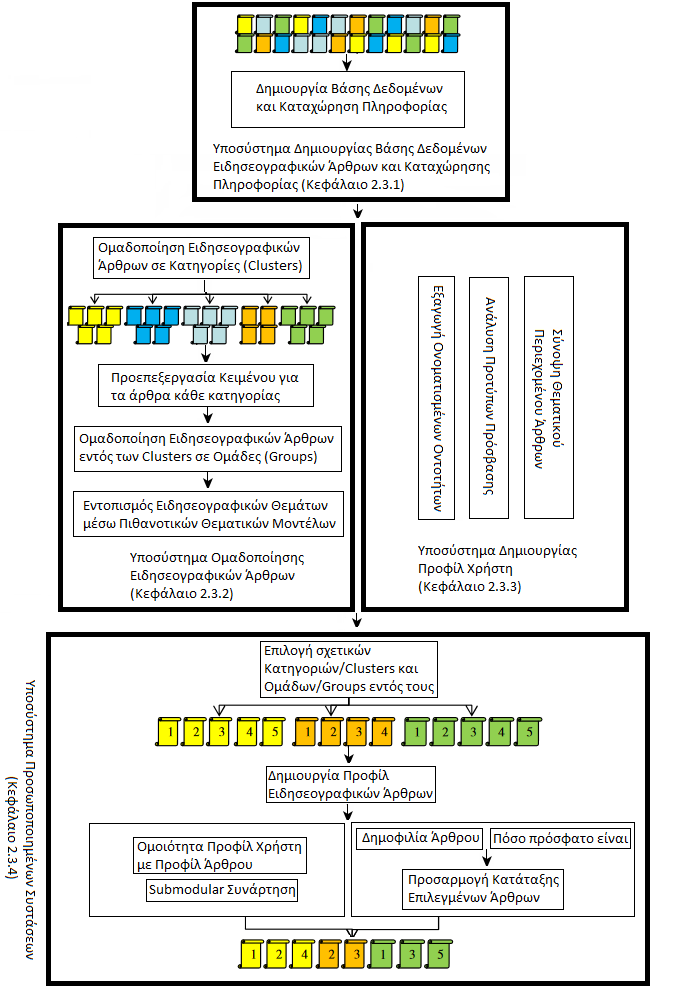
\includegraphics[scale=0.77]{static/figures/arch1.png}
    \caption{Αρχιτεκτονική Συστήματος}
    \label{}
\end{figure} 

\section{Υποσυστήματα}

Στη συνέχεια παρουσιάζουμε τα διάφορα υποσυστήματα από τα οποία αποτελείται ο
μηχανισμός προκειμένου να γίνει κατανοητή η λειτουργία του.

\begin{enumerate}

  \item Υποσύστημα Δημιουργίας Βάσης Δεδομένων και Καταχώρησης Πληροφορίας
    \begin{itemize}
      \item{Συλλογή Ειδησεογραφικών Άρθρων}
      \item{Δημιουργία Βάσης Δεδομένων και Καταχώρηση Πληροφορίας}
      \end{itemize}
  
  \item Υποσύστημα Ομαδοποίησης Ειδησεογραφικών Άρθρων
    \begin{itemize}
    \item{Ομαδοποίηση Ειδησεογραφικών Άρθρων σε Κατηγορίες {\en {(Clusters)}}}
    \item{Προεπεξεργασία Κειμένου {\en {(Text Preprocessing)}}}
    \item{Ομαδοποίηση Ειδησεογραφικών Άρθρων εντός των {\en {Clusters}} σε Ομάδες {\en {(Groups)}}}
    \item{Εντοπισμός Ειδησεογραφικών Θεμάτων μέσω Πιθανοτικών Θεματικών Μοντέλων}
  \end{itemize}
  
  \item Υποσύστημα Δημιουργίας Προφίλ Χρήστη
    \begin{itemize}
      \item Σύνοψη Θεματικού Περιεχομένου Άρθρων
      \item Ανάλυση Προτύπων Πρόσβασης
      \item Εξαγωγή Ονοματισμένων Οντοτήτων
    \end{itemize}

  \item Υποσύστημα Προσωποποιημένων Συστάσεων
    \begin{itemize}
     \item Αντιστοίχιση Αναγνωστικών Προτιμήσεων για την Αναπαράσταση 1ου Επιπέδου
     \item Αντιστοίχιση Αναγνωστικών Προτιμήσεων για την Αναπαράσταση 2ου Επιπέδου
     \begin{enumerate}
      \item Δημιουργία Προφίλ Ειδησεογραφικών Άρθρων
      \item Εισαγωγή στις {\en {Submodular}} Συναρτήσεις
      \item Μοντέλο Συστάσεων
      \item Προσαρμογή Κατάταξης Ειδησεογραφικών Άρθρων
      \end{enumerate}
    \end{itemize}

\end{enumerate}

Παρακάτω δίνεται λεπτομερής περιγραφή για καθένα από τα υποσυστήματα που αναφέραμε.

% **********************************************************
\subsection{Υποσύστημα Δημιουργίας Βάσης Δεδομένων και Καταχώρησης Πληροφορίας}
% **********************************************************

Η συλλογή των άρθρων ανακτήθηκε κατά βάση από το διαδίκτυο από αρκετές διαδικτυακές υπηρεσίες ειδήσεων, 
όπως οι εξής: {\textit {{\en {The Guardian, New York Times, Washington Post, Fox News, Independent, Reuters, Sky News}}}. 
Ένα μέρος της συλλογής προήλθε από τη συλλογή άρθρων {\textit {{\en {Reuters}}} του {\en {NLTK}}.

Μετά την ολοκλήρωση της διαδικασίας συλλογής, 
δημιουργούμε τη βάση δεδομένων και αποθηκεύουμε τα άρθρα στους αντίστοιχους πίνακες της βάσης του συστήματος.
Οι πληροφορίες που αποθηκεύονται για κάθε άρθρο είναι: 
τίτλος, συγγραφέας, ημερομηνία δημοσίευσης, κείμενο άρθρου, γενική κατηγορία ({\en {cluster}}) στην οποία ανήκει το κάθε άρθρο. \\
Επιπρόσθετα, στο αρχικό αυτό στάδιο, δημιουργούμε και καταχωρούμε μία σειρά από χρήστες του συστήματος. 
Συγκεκριμένα, κατά τη δημιουργία της βάσης δεδομένων παράγεται αυτόματα ένα αναγνωστικό ιστορικό για κάθε αποθηκευμένο χρήστη, 
τόσο ελεγχόμενα όσο και τυχαία και αποθηκεύεται στον αντίστοιχο πίνακα της βάσης. 
Ως προς το ελεγχόμενο μέρος επιχειρούμε να ταιριάξουμε κάθε αποθηκευμένο χρήστη με μία συγκεκριμένη κατηγορία άρθρων, 
φορτώνοντας στο αναγνωστικό ιστορικό του μέσω ενός αρχείου μεγαλύτερο αριθμό άρθρων από κάποια συγκεκριμένη κατηγορία. 
Μέσω του ελεγχόμενου τρόπου καταφέρνουμε να διασφαλίσουμε ότι κάθε άρθρο της βάσης δεδομένων θα έχει αναγνωσθεί 
τουλάχιστον μία φορά από κάποιον τυχαίο χρήστη.
Ως προς το τυχαίο μέρος επιλέγουμε μέσω της συνάρτησης {\en {\textit{rand}} και έναν τυχαίο (εντός ορίων) αριθμό άρθρων από οποιαδήποτε κατηγορία 
για να εμπλουτίσουμε το περιεχόμενο του αναγνωστικού ιστορικού του χρήστη. \\

Πλέον, έχουμε συλλέξει στη βάση δεδομένων όλη την απαραίτητη πληροφορία για το επόμενο υποσύστημα.

% **********************************************************
\subsection{Υποσύστημα Ομαδοποίησης Ειδησεογραφικών Άρθρων}
% **********************************************************

Τυπικά, δεδομένου ενός σετ ειδησεογραφικών άρθρων {\en {\textit{N = \{$n_1, n_2, ..., n_M$\}}}}, 
όπου {\en {\textit{$\vert N\vert$ = M}}}, στόχος μας είναι μια στιβαρή ομαδοποίηση {\en {(hard clustering)
C = \{$C_1, C_2, ..., C_K$\}}} στο {\en {\textit{N}}, όπου το {\en {\textit{K}} είναι ένας προκαθορισμένος 
αριθμός από {\en {clusters}}. Κάθε {\en {cluster}} {\en {\textit{$C_i$}}} αποτελείται από μία λίστα από {\en {groups}} 
ειδησεογραφικών άρθρων {\en {G = \{$G_1, G_2, ...$\}}} και κάθε {\en {group}} {\en {\textit{$G_j$}}} 
περιέχει {\en {\textit{$t_j$}}} ειδησεογραφικά άρθρα. 
Κάθε {\en {cluster}} καθώς και τα {\en {groups}} άρθρων που περιλαμβάνει είναι αντιστοίχως συσχετισμένα 
με μία κατανομή θεμάτων {\en {\textit{T}}}, η οποία περιγράφει τα θέματα που “κρύβονται” μέσα στα άρθρα. 
Στόχος της συγκεκριμένης αναπαράστασης είναι ο εξής: 
Οι προσωποποιημένες συστάσεις άρθρων απαιτούν γρήγορη απόκριση για να παρουσιάσουν 
άμεσα αποτελέσματα στους χρήστες. Η συγκεκριμένη αναπαράσταση άρθρων μπορεί να βοηθήσει 
στη γρήγορη πλοήγηση προς άρθρα που ενδιαφέρουν το χρήστη. 

% ____________________________________________
\subsubsection{Ομαδοποίηση Ειδησεογραφικών Άρθρων σε Κατηγορίες {\en {(Clusters)}}}
% ____________________________________________

Δεδομένου του τρόπου συλλογής των άρθρων που βρίσκονται αποθηκευμένα στη βάση δεδομένων του συστήματος, 
γνωρίζουμε εκ των προτέρων την κατηγορία στην οποία ανήκουν το κάθε ένα από αυτά. 
Έτσι, είτε πρόκειται για άρθρα που προέρχονται από διαδικτυακές υπηρεσίες ειδήσεων, 
είτε για άρθρα από τη συλλογή {\en {Reuters}} του {\en {NLTK}}, κάθε ένα είναι εξαρχής συσχετισμένο 
με μια συγκεκριμένη κατηγορία από το σύνολο των διαφορετικών κατηγοριών που έχουμε επιλέξει. \\
Στο σύστημά μας εμφανίζονται άρθρα από εφτά διαφορετικές κατηγορίες. 
Κάθε κατηγορία σχετίζεται με ένα από τα παρακάτω θέματα: 
\textit{{\en {Science/Technology, Politics, Sports, Life \& Style, Sugar, Coffee, Housing}}}. 
Οι τέσσερις πρώτες κατηγορίες περιλαμβάνουν άρθρα που συλλέχθηκαν από το διαδίκτυο, 
ενώ οι υπόλοιπες τρεις κατηγορίες αποτελούνται από άρθρα της συλλογής {\en {Reuters}}.\\
Σε αυτό το στάδιο της προεπεξεργασίας της συλλογής κειμένων μπορούμε να θεωρήσουμε με βεβαιότητα 
ότι αυτή η πρώτη ομαδοποίηση που πραγματοποιήθηκε πάνω στη συλλογή κειμένων είναι και η πιο αποτελεσματική, 
καθώς έχουμε εξασφαλίσει ότι τα ειδησεογραφικά άρθρα με κοινό θεματικό περιεχόμενο ανήκουν στο ίδιο {\en {cluster}}. \\
Τέλος, είναι σαφές ότι κάθε άρθρο ανήκει αποκλειστικά σε ένα και μοναδικό {\en {cluster}}. 
\\

Παρακάτω προχωρούμε σε περαιτέρω ομαδοποίηση των άρθρων, αυτή τη φορά εντός των {\en {clusters}} που δημιουργήσαμε, 
με σκοπό τη δημιουργία της βάσης του πρώτου επιπέδου σύστασης ειδησεογραφικών άρθρων του συστήματός μας. 

% ____________________________________________
\subsubsection{Προεπεξεργασία Κειμένου {\en {(Text Preprocessing)}}}
% ____________________________________________

Πρωτού προβούμε σε εφαρμογή του αλγορίθμου ομαδοποίησης των άρθρων εντός των  {\en {clusters}} σε ομάδες {\en {(groups)}}, 
κρίνεται απαραίτητη η προεπεξεργασία των κειμένων των άρθρων κάνοντας χρήση της βιβλιοθήκης {\en {scikit-learn}} της {\en {Python}}. 
Η πληροφορία που δίνεται σαν είσοδος στο μηχανισμό προέρχεται από τη βάση δεδομένων του συστήματος 
και αποτελείται από τα κείμενα των άρθρων κάθε {\en {cluster}}. 
Πρωταρχικός σκοπός μας στο στάδιο αυτό είναι η απομάκρυνση ανεπιθύμητων συμβολοσειρών μέσω φιλτραρίσματος των λέξεων 
που δε φέρουν ουσιαστική πληροφορία και η ανάλυση του κειμένου για την εξαγωγή λέξεων-κλειδιών από το κείμενο του κάθε άρθρου.
Βασικά σημεία προεπεξεργασίας: 
\begin{itemize}
 \item \textbf{Λεξική Ανάλυση}: Το στάδιο αυτό αφορά τον διαμερισμό κάθε άρθρου στα συστατικά στοιχεία του κειμένου του {\en {(tokenization)}}, 
 μετατρέποντας το κείμενο σε ακολουθία λέξεων. 
 \item \textbf{Αφαίρεση τετριμμένων λέξεων και τερματικών όρων {\en {(stopwords)}}}: Για κάθε άρθρο της συλλογής πραγματοποιείται καθαρισμός 
 από τετριμμένες λέξεις {\en {(elimination of insignificant words)}}, 
όπως είναι τα άρθρα, οι σύνδεσμοι, οι αντωνυμίες, καθώς και οι συχνά χρησιμοποιούμενες λέξεις 
που δεν ανήκουν στις ανωτέρω κατηγορίες, αλλά δεν φέρουν καμία ιδιαίτερη σημασιολογική πληροφορία, 
όπως είναι ορισμένα επιρρήματα. Ένα {\en {stopword}} είναι μια συχνά χρησιμοποιούμενη λέξη, 
όπως οι {\en {``the'', ``and'', ``to'', ``also''}}, όπου μία μηχανή αναζήτησης έχει σχεδιαστεί να αγνοεί, 
τόσο κατά την ευρετηρίαση των καταχωρήσεων προς αναζήτηση, όσο και κατά την ανάκτησή τους ως αποτελέσματα μιας αναζήτησης. 
Δεν επιθυμούμε αυτές οι λέξεις να καταλαμβάνουν χώρο στη βάση δεδομένων 
ή να κατασπαταλούν πολύτιμο υπολογιστικό χρόνο, καθότι φέρουν ελάχιστον λεκτικό 
περιεχόμενο και η παρουσία τους σε ένα κείμενο δε διευκολύνει τη διάκριση του κειμένου από άλλα κείμενα. 
Το {\en {NLTK}} περιέχει μία λίστα από {\en {stopwords}} αποθηκευμένα σε δεκαέξι διαφορετικές γλώσσες.
Στο σημείο αυτό απομακρύνουμε, επίσης, τα αριθμητικά δεδομένα και τα σημεία στίξης.
 \item \textbf{Κανονικοποίηση των λέξεων}: Το στάδιο αυτό αφορά την αναγνώριση των ριζών των λέξεων, 
 γνωστή ως λημματοποίηση {\en {(lemmatization)}} και την αποκατάληξη {\en {(stemming)}}, 
ώστε να μην επηρεάζεται η εξαγωγή χαρακτηριστικών γνωρισμάτων των κειμένων από την πτώση ή το χρόνο που κλίνονται οι λέξεις. 
Έτσι, καταλήγουμε σε αναγωγή όλων των μορφολογικών τύπων μίας λέξης σε μία ενιαία αναπαράσταση. 
\item \textbf{Επιλογή των αντιπροσωπευτικών όρων}: Στη συνέχεια, η διαδικασία βασίζεται στην εξαγωγή χαρακτηριστικών γνωρισμάτων (λέξεων–κλειδιών) των κειμένων, η οποία αφορά την
εφαρμογή μέτρων ποιότητας για την επιλογή διατήρησης ορισμένων όρων για κάθε κείμενο. 
Η εξαγωγή των λέξεων–κλειδιών των κειμένων γίνεται μέσω του εργαλείου {\en {TfidfVectorizer}} \cite{Tfidf01}
της βιβλιοθήκης {\en {scikit-learn}} της {\en {Python}}. Η εξαγωγή των σωστών λέξεων-κλειδιών είναι πολύ σημαντική. \\
Η μέθοδος \textbf{{\en {TF–IDF}}} \cite{Tfidf02} είναι μια μετρική που δηλώνει πόσο σημαντικός είναι ένας όρος σε ένα έγγραφο από μια συλλογή εγγράφων. 
Η μέθοδος {\en {TF–IDF}} στοχεύει στο να σταθμίσει όλους τους όρους μιας συλλογής κειμένων. 
Με λίγα λόγια, στόχος της είναι να αποδώσει το αντίστοιχο βάρος σε κάθε όρο και, κατά επέκταση, σε κάθε διάσταση του πολυδιάστατου αυτού χώρου. 
Αυτό συμβαίνει γιατί η απλή αρίθμηση ενός όρου σε ένα κείμενο δεν αρκεί για να μας πληροφορήσει 
για τη σημαντικότητα του όρου αυτού και τη βαρύτητα της πληροφορίας που περιέχει. \\
Η μέθοδος αυτή αποτελείται από τις ποσότητες {\en {TF}} και {\en {IDF}}. 
Η ποσότητα {\en {TF}} (συχνότητα όρου) υποδηλώνει το πόσες φορές εμφανίζεται ένας όρος σε ένα κείμενο. 
Από την άλλη, η ποσότητα {\en {IDF}} υποδηλώνει το πόσο ένας όρος είναι διαδεδομένος σε 
ένα κείμενο αλλά και σε ολόκληρη τη συλλογή κειμένων. 
Τελικά, το βάρος ενός όρου προκύπτει από τον πολλαπλασιασμό των ποσοτήτων {\en {TF}} και {\en {IDF}}. \\
Στόχος της μεθόδου αυτής μέσω του βάρους είναι η επιλογή εκείνων των όρων που αποτυπώνουν καλύτερα το περιεχόμενο ενός κειμένου.
Για τον προσδιορισμό του βάρους ενός όρου είναι εξίσου σημαντικές και οι δύο ποσότητες 
{\en {TF}} και {\en {IDF}}.
Αυτό επισημαίνεται διότι αν χρησιμοποιούσαμε μόνο τη συχνότητα εμφάνισης ενός όρου ({\en {TF}}) ως βάρος,
αυτό θα είχε ως συνέπεια οι συχνότερα εμφανιζόμενοι όροι να θεωρούνται ως οι πιο σημαντικοί. 
Αυτή η υπόθεση θα μπορούσε να μας οδηγήσει σε λανθασμένη επιλογή 
όρων οι οποίοι εμφανίζονται σε πολλά κείμενα και δεν προσφέρουν κάποια ιδιαίτερη πληροφορία σε ένα κείμενο. 
Για παράδειγμα, η λέξη «εξόρυξη» σε μία συλλογή κειμένων με θέμα «Τεχνικές Εξόρυξης Κειμένων» 
θα εμφανίζεται με μεγάλη συχνότητα σε όλα τα κείμενα της συλλογής. 
Επομένως, μέσα από αυτό το παράδειγμα καταλαβαίνουμε πως ένας τέτοιος όρος, παρότι θα μπορούσε 
να εμφανίζεται αρκετές φορές σε ένα κείμενο, δε θα μπορούσε να θεωρηθεί ως ένας σημαντικός όρος,
γιατί δεν προσφέρει ένα ιδιαίτερο χαρακτηριστικό στο  κείμενο σε σχέση με τα υπόλοιπα κείμενα της συλλογής.
Εδώ, λοιπόν, καταλαβαίνουμε τη σημαντικότητα της ποσότητας {\en {IDF}} στον υπολογισμό του βάρους ενός όρου. 
Όταν ένας όρος εμφανίζεται σε πολλά κείμενα της συλλογής, η τιμή της ποσότητας {\en {IDF}} είναι μικρή, 
ενώ όταν ένας όρος εμφανίζεται σε λίγα κείμενα της συλλογής, η τιμή της ποσότητας {\en {IDF}} είναι μεγάλη. \\
Επομένως, μεγάλο βάρος για έναν όρο προκύπτει όταν ο όρος αυτός εμφανίζεται πολλές φορές σε ένα κείμενο 
και λιγότερες φορές στο σύνολο των κειμένων. \\
\end{itemize}

Χρησιμοποιώντας τη διαδικασία που περιγράψαμε παραπάνω, ο μηχανισμός διαβάζει
καινούργια άρθρα από τη βάση δεδομένων του συστήματος ανά κατηγορία {\en {(cluster)}}, 
εξάγει τις λέξεις–κλειδιά για κάθε άρθρο της κατηγορίας και τις συσχετίζει με το άρθρο και το αντίστοιχο βάρος. 
Έχοντας ολοκληρώσει την προεπεξεργασία των κειμένων της συλλογής, 
τα δεδομένα μας έχουν πλέον την κατάλληλη μορφή ώστε να προχωρήσουμε στη διαδικασία ομαδοποίησης 
των άρθρων εντός της κάθε κατηγορίας {\en {(cluster)}}. 

% ____________________________________________
\subsubsection{Ομαδοποίηση Ειδησεογραφικών Άρθρων εντός των {\en {Clusters}} σε Ομάδες {\en {(Groups)}}}
% ____________________________________________

\par Τα ειδησεογραφικά άρθρα που περιέχονται σε κάθε {\en {cluster}} επικεντρώνονται σε παρόμοιες πτυχές ενός γενικού θέματος, 
εκείνου που αντιπροσωπεύεται από τον τίτλο της εκάστοτε κατηγορίας. 
Τυπικά, ένας χρήστης ενδιαφέρεται για συγκεκριμένες πτυχές ενός θέματος και όχι για όλες. 
Βασισμένοι σε αυτή την παραδοχή και με στόχο την γρήγορη πλοήγηση, κατά το στάδιο σύστασης, προς άρθρα που ενδιαφέρουν το χρήστη, 
προχωρούμε σε περαιτέρω ομαδοποίηση των άρθρων εντός κάθε κατηγορίας με σκοπό τη δημιουργία ομάδων {\en {(groups)}} εντός κάθε {\en {cluster}}. \\

% sklearn.cluster KMeans
H ομαδοποίηση εντός κάθε {\en {cluster}} πραγματοποιείται με εφαρμογή του αλγορίθμου {\en {k-means}} με βάση κάποιο μέτρο ομοιότητας, 
με στόχο όλα τα άρθρα που ανήκουν στην ίδια ομάδα να είναι παρόμοια μεταξύ τους. 
Για την εφαρμογή του αλγορίθμου γίνεται χρήση της βιβλιοθήκης {\en {scikit-learn}} της {\en {Python}}. \\

\par O αλγόριθμος \textbf{{\en {k-means}}} \cite{Km01} είναι ο πιο διαδεδομένος αλγόριθμος ομαδοποίησης. 
O {\en {k-means}} διασπάει τα δεδομένα σε {\en {k}} διαφορετικές ομάδες μέσω μίας επαναληπτικής διαδικασίας, 
όπου {\en {k}} είναι ένας προκαθορισμένος ακέραιος αριθμός και παρέχεται από εμάς. 
Η επαναληπτική διαδικασία τερματίζει τη στιγμή που θα ικανοποιηθεί ένα συγκεκριμένο κριτήριο. 
Τα κύρια βήματα του αλγορίθμου περιγράφονται παρακάτω: 

\begin{enumerate}
 \item Αρχικά, γίνεται η επιλογή {\en {k}} σημείων στο πεδίο των δεδομένων έτσι ώστε τα σημεία αυτά 
 να αποτελούν τα κέντρα των αρχικών ομάδων. 
 \item Ανάθεσε κάθε δεδομένο σε μία ομάδα για το οποίο η απόστασή του από το κέντρο της ομάδας να είναι 
 η μικρότερη από κάθε άλλη εκ των κέντρων των υπολοίπων ομάδων. 
 \item Όταν όλα τα δεδομένα έχουν ανατεθεί στις ομάδες, υπολόγισε ξανά τα κέντρα των ομάδων, παίρνοντας 
 το μέσο όρο των δεδομένων κάθε ομάδας. 
 \item Επανάλαβε τα βήματα 2, 3 μέχρι να επαληθευτεί κάποιο κριτήριο σύγκλισης.
\end{enumerate}

Το κριτήριο σύγκλισης του αλγορίθμου, ο τρόπος μέτρησης της απόστασης των δεδομένων από τα κέντρα των ομάδων, 
καθώς και ο τρόπος ανάδειξης των αρχικών κέντρων τους καθορίζουν σε μεγάλο βαθμό την τελική ομαδοποίηση των δεδομένων 
και ορίζονται από το χρήστη. \\

% Μετά από δοκιμές με σκοπό την ανεύρεση του καταλληλότερου αριθμού k

% ********************************* +++

Τα ήδη υπάρχοντα {\en {clusters}} μαζί με τα παραγόμενα {\en {groups}} που περιέχονται σε αυτά 
αποτελούν τη βάση του πρώτου επιπέδου σύστασης ειδησεογραφικών άρθρων του συστήματός μας. 

% ____________________________________________
\subsubsection{Εντοπισμός Ειδησεογραφικών Θεμάτων μέσω Πιθανοτικών Θεματικών Μοντέλων}
% ____________________________________________

Ένας φυσικός τρόπος να εξερευνήσουμε τους συσχετισμούς μεταξύ των {\en {clusters} (ή των {\en {groups}) άρθρων 
και του προφίλ του δοθέντος χρήστη είναι να συγκρίνουμε την ομοιότητα των θεμάτων που “κρύβονται” μέσα στα άρθρα τους. 
Γενικά, η ανακάλυψη κρυμμένων θεμάτων που υπάρχουν σε μια συλλογή κειμένων πραγματοποιείται χρησιμοποιώντας 
πιθανοτικά μοντέλα θεμάτων, όπως τα {\en {PLSI}} και {\en {LDA}} \cite{Lda02}, εξάγοντας μια λίστα αντιπροσωπευτικών λέξεων 
από την αρχική συλλογή κειμένων μαζί με το αντίστοιχο βάρος για κάθε λέξη. 
Τα μοντέλα θεμάτων μοντελοποιούν κάθε αντικείμενο μιας συλλογής ως ένα πεπερασμένο μείγμα από ένα σύνολο θεματικών πιθανοτήτων. \\

Ένα γενετικό {\en {(generative)}} μοντέλο θεμάτων βασίζεται στους απλούς πιθανοτικούς κανόνες επιλογής {\en {(sampling)}} 
που περιγράφουν πως οι λέξεις μέσα στα κείμενα μπορεί να δημιουργηθούν μέσω τυχαίων κρυφών μεταβλητών. 
Όταν προσαρμόζουμε ένα γενετικό μοντέλο, ο στόχος είναι να βρεθεί το καταλληλότερο σύνολο κρυφών μεταβλητών 
που μπορεί να εξηγήσει τα παρατηρούμενα δεδομένα υποθέτοντας ότι το μοντέλο δημιουργήθηκε από τα δεδομένα. 
Το Σχήμα \ref{fig:ldamodel01} δείχνει την προσέγγιση μοντέλων θεμάτων με δύο τρόπους: 
σαν γενετικό μοντέλο και σαν πρόβλημα μεταβολικής συμπερασματολογίας. 
Στα αριστερά, η γενετική διαδικασία παρουσιάζεται με δύο θέματα {\en {(topics)}}. 
Τα {\en {Topic}} 1 και 2 είναι θεματικά συσχετισμένα με το {\en {'money'}} και τα {\en {'rivers'}} 
και απεικονίζονται σαν τσάντες που περιέχουν διαφορετικές κατανομές ως προς τις λέξεις. 
Διαφορετικά κείμενα μπορούν να παραχθούν επιλέγοντας λέξεις από ένα θέμα δεδομένου του βάρους που έχει. 
Για παράδειγμα, τα κείμενα {\en {Doc1}} και {\en {Doc3}} έχουν δημιουργηθεί με την διαδικασία \textit{{\en {sampling}}} 
μόνο από το {\en {topic}} 1 και το {\en {topic}} 2 αντίστοιχα, 
ενώ το κείμενο {\en {Doc2}} δημιουργήθηκε από την ίση μείξη των δύο θεμάτων. 
Με τον τρόπο όπου το μοντέλο ορίστηκε, δεν υπάρχει κάποια αμοιβαία αποκλειστικότητα 
που να περιορίζει τις λέξεις να είναι μέρος ενός μόνο θέματος. 
Αυτό επιτρέπει στο μοντέλο να καταλαβαίνει την πολυσημία, δηλαδή τις  πολλές σημασίες όπου η ίδια η λέξη μπορεί να έχει ταυτόχρονα. 
Για παράδειγμα, και τα δύο θέματα {\en {'money'}} και {\en {'rivers'}} δίνουν υψηλή πιθανότητα στην λέξη \textit{{\en {bank}}}, 
που είναι λογικό, δεδομένης της πολυσημικής φύσης της λέξης.\\

\begin{figure}[!ht] \centering
\centerline{
    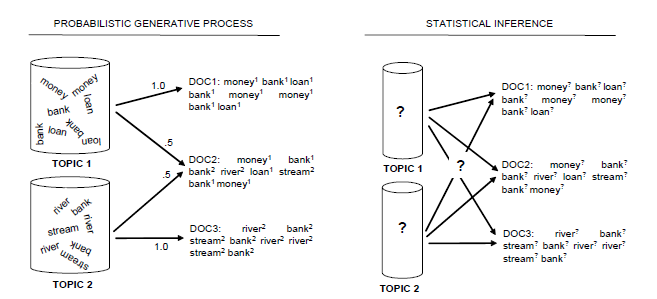
\includegraphics[scale=0.75]{static/figures/model.png}}
    \caption{Απεικόνιση γενετικής διαδικασίας και του προβλήματος στατιστικής συμπερασματολογίας 
    που λύνεται με μοντέλα θεμάτων.}
    \label{fig:ldamodel01}
\end{figure}

Στο σύστημά μας εφαρμόζουμε το \textbf{{\en {LDA (Latent Dirichlet Allocation)}}} ως το μοντέλο για την ανακάλυψη κρυμμένων θεμάτων 
και αναπαριστούμε την κατανομή θεμάτων ως ένα διάνυσμα κάθε εγγραφή του οποίου δηλώνει το βάρος της αντίστοιχης λέξης. 
Για την εφαρμογή του {\en {LDA}} μοντέλου γίνεται χρήση της βιβλιοθήκης {\en {gensim}} \cite{Lda01} της {\en {Python}}. \\

Ο αλγόριθμος ανάλυσης κειμένων {\en {LDA}} αποτελεί ένα πιθανοτικό μοντέλο που επιτρέπει την
ερμηνεία κάποιων δεδομένων μέσα από κάποια σύνολα παρατηρήσεων. 
Για παράδειγμα, αν οι παρατηρήσεις είναι λέξεις που έχουν συλλεχθεί από κάποια κείμενα, 
ο αλγόριθμος θεωρεί ότι τα κείμενα αντιπροσωπεύονται από τυχαίες προσμείξεις
κρυφών θεμάτων, όπου κάθε θέμα χαρακτηρίζεται από μία κατανομή ως προς τις λέξεις.
% κάθε κείμενο είναι μία ανάμειξη από έναν μικρό αριθμών θεμάτων. 
Ο {\en {LDA}} είναι ένα παράδειγμα μοντέλου θεμάτων και παρουσιάστηκε για πρώτη φορά ως γενετικό
μοντέλο ανακάλυψης θεμάτων από τους {\en {David Blei, Andrew Ng}} και {\en {Michael Jordan}} το 2002.
Κύριο πλεονέκτημα του {\en {LDA}}, καθώς και των παραλλαγών του, είναι ο μεγάλος βαθμός
προσαρμογής τους. Έτσι, μπορούν να εφαρμοστούν και σε διάφορα άλλα προβλήματα που
αντικείμενα απασχόλησης δεν είναι κείμενα λέξεων. Για παράδειγμα, ο αλγόριθμος έχει
χρησιμοποιηθεί στο πεδίο της μηχανική όρασης για ανάλυση εικόνας, στο πεδίο της
βιοπληροφορικής για ανάλυση και ανάκτηση γενετικού κώδικα σε δεδομένα ερευνών κ.α. 
Στόχος μας είναι να βρούμε σύντομες περιγραφές των μελών της συλλογής 
που επιτρέπουν μια αποτελεσματική επεξεργασία μεγάλων συλλογών, 
διατηρώντας τις απαραίτητες στατιστικές σχέσεις που είναι χρήσιμες
για βασικές διεργασίες όπως η περίληψη κειμένου.

\begin{figure}[!ht] \centering
\centerline{
    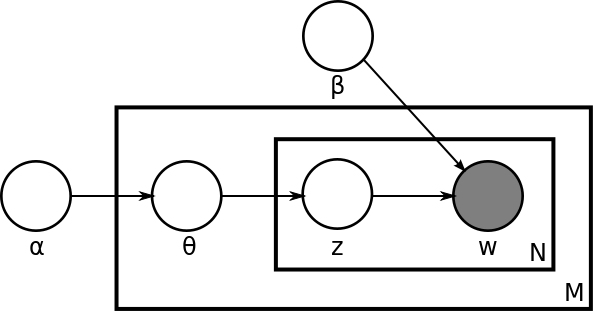
\includegraphics[scale=0.45]{static/figures/ldamodel2.png}}
    \caption{Γραφικό μοντέλο απεικόνισης του {\en {LDA}}. Τα πλαίσια απεικονίζουν τις επαναλήψεις. 
    Το εξωτερικό πλαίσιο απεικονίζει τα κείμενα, ενώ το εσωτερικό την επαναληπτική επιλογή των θεμάτων 
    και των λέξεων μέσα σε ένα κείμενο.}
    \label{fig:ldamodel02}
\end{figure}

Το {\en {LDA}} μοντέλο απεικονίζεται ως πιθανοτικό γραφικό μοντέλο στην εικόνα \ref{fig:ldamodel02}. 
Όπως γίνεται αντιληπτό από την εικόνα, υπάρχουν τρία επίπεδα στο {\en {LDA}}. 
Οι παράμετροι α και β είναι επιπέδου σώματος παράμετροι, που έχουν συλλεχθεί 
από την διαδικασία δημιουργίας του σώματος. 
Οι μεταβλητές θ είναι επιπέδου κειμένου μεταβλητές, που έχουν ληφθεί από ένα κείμενο. 
Τέλος, οι μεταβλητές {\en {z}} και {\en {w}} είναι επιπέδου λέξεων μεταβλητές και έχουν συλλεχθεί για κάθε λέξη κάθε κειμένου. 
Οι μεταβλητές {\en {M, N}} δηλώνουν αντίστοιχα τον αριθμό των κειμένων και τον αριθμό των λέξεων μέσα σε ένα κείμενο.

Είναι απαραίτητο να ξεχωρίσουμε το {\en {LDA}} από το απλό {\en {Dirichlet}} πολυωνυμικό μοντέλο ομαδοποίησης. 
Ένα κλασσικό μοντέλο ομαδοποίησης θα ήταν ένα δύο-επιπέδων μοντέλο, 
όπου η {\en {Dirichlet}} θα υπολογιζόταν μία φόρα για ένα σώμα, μια πολυωνυμική μεταβλητή
ομαδοποίησης θα επιλεγόταν για κάθε κείμενο του σώματος και ένα σύνολο λέξεων
θα επιλεγόταν για ένα κείμενο της μεταβλητής ομάδας. Όπως και με πολλά αλλά μοντέλα
ομαδοποίησης, ένα τέτοιο μοντέλο περιορίζει ένα κείμενο στο να συσχετίζεται μόνο με ένα θέμα. 
Αντιθέτως, το {\en {LDA}} είναι μοντέλο τριών επιπέδων και ο θεματικός κόμβος επιλέγεται επαναλαμβανόμενα από κάθε κείμενο. 
Με αυτό το μοντέλο τα κείμενα μπορούν να συσχετιστούν με πολλά θέματα. \\

\nocite{RecommendLda, Lda03, Scenepaper, Exp01, Hybrid, Adapt, Mining}

Στο σημείο αυτό, έχοντας αναλύσει το θεωρητικό υπόβαθρο γύρω από τα πιθανοτικά θεματικά μοντέλα και συγκεκριμένα το μοντέλο {\en {LDA}}, 
προχωράμε στην εφαρμογή του {\en {LDA}} σε κάθε {\en {cluster}} (κατηγορία) άρθρων, σε κάθε {\en {group}} εντός των {\en {clusters}}, 
καθώς και σε κάθε μεμονωμένο άρθρο.
Έτσι, καταλήγουμε με το διάνυσμα της κατανομής θεμάτων τόσο για τα άρθρα, όσο και για τα {\en {clusters}} και τα {\en {groups}} που έχουν δημιουργηθεί. 
Κάθε καταχώρηση ενός τέτοιου διανύσματος θεμάτων αποτελείται από μία αντιπροσωπευτική λέξη και το αντίστοιχο βάρος. 
Κατά την εφαρμογή του αλγορίθμου μπορούμε να επιλέξουμε τον αριθμό αντιπροσωπευτικών λέξεων απ'τις οποίες θα αποτελείται ένα τέτοιο διάνυσμα. 
% Στο κώδικά μας επιλέξαμε να κρατάμε τις σαράντα πιο κατάλληλες λέξεις για κάθε {\en {cluster, group}} και άρθρο, μαζί με τα αντίστοιχα βάρη τους. 

% **********************************************************
\subsection{Υποσύστημα Δημιουργίας Προφίλ Χρήστη}
% **********************************************************

Ένα από τα ιδιαίτερα χαρακτηριστικά ενός συστήματος δημιουργίας εξατομικευμένων
συστάσεων είναι το Προφίλ Χρήστη (στο πλαίσιο των συστημάτων συστάσεων). Το
Προφίλ Χρήστη είναι μια αναπαράσταση των πληροφοριών που υπάρχουν για ένα
χρήστη, οι οποίες είναι απαραίτητες για ένα προσαρμοζόμενο σύστημα ώστε αυτό να
προσφέρει εξατομίκευση, δηλαδή να συμπεριφέρεται διαφορετικά για διαφορετικούς
χρήστες. \\

Παραδοσιακά, το προφίλ ενός χρήστη μπορεί να καθοριστεί παρακολουθώντας τα άρθρα 
τα οποία έχουν διαβαστεί από το χρήστη μέχρι στιγμής (ιστορικό περιήγησης), με βάση το περιεχόμενο των άρθρων. 
Ο τρόπος αναπαράστασης του προφίλ εξαρτάται από τη μέθοδο που χρησιμοποιεί το σύστημα πρόσβασης.
Ουσιαστικά, το προφίλ αποτελεί ένα σύνολο των πιθανών ενδιαφερόντων του χρήστη.
Παρ\textquotesingleόλ\textquotesingleαυτά, η προσέγγιση αυτή δεν αποτυπώνει αποτελεσματικά τις ακριβείς αναγνωστικές προτιμήσεις του χρήστη, 
καθώς το ενδιαφέρον του ενδέχεται να επηρεάζεται και από τις προτιμήσεις άλλων χρηστών. 
Επιπρόσθετα, η ανεπάρκεια της προσέγγισης στηριζόμενης αποκλειστικά στο περιεχόμενο των άρθρων 
οφείλεται και στο γεγονός ότι πολλοί χρήστες τείνουν να επιλέγουν άρθρα επηρεασμένοι 
από φράσεις/ονοματισμένες οντότητες όπως οι εξής: Τι συνέβη, ποιος εμπλέκεται, πότε συνέβη κ.λπ. \\

Στηριζόμενοι στην παραπάνω ανάλυση, το Προφίλ Χρήστη παραμετροποιείται μέσω μιας τριπλέτας {\en {\textit{U = $\langle$T, P, E $\rangle$}}} 
αποτελούμενης από τα εξής χαρακτηριστικά: 
\begin{itemize}
\item Το {\en {\textit{T}}} αναπαριστά την κατανομή των θεμάτων των ειδησεογραφικών άρθρων τα οποία ο χρήστης έχει διαβάσει στο παρελθόν, 
με μορφή διανύσματος θεμάτων {\en {\textit{\{$\langle$t1, w1$\rangle$, $\langle$t2, w2$\rangle$, ...\}}}}, όπου κάθε καταχώρηση του διανύσματος 
αποτελείται από μια αντιπροσωπευτική λέξη και το αντίστοιχο βάρος. 
\item Το {\en {\textit{P}}} δηλώνει μια λίστα χρηστών {\en {\textit{\{$\langle$u1, u2, ...$\rangle$\}}}} οι οποίοι έχουν παρόμοια πρότυπα πρόσβασης.
\item Το {\en {\textit{E}}} είναι μια λίστα από ονοματισμένες οντότητες {\en {\textit{\{$\langle$e1, e2, ...$\rangle$\}}}} εξαγόμενες από 
το ιστορικό αναγνωσμένων άρθρων του χρήστη, συσχετισμένες με τον αντίστοιχο τύπο οντότητας. 
\end{itemize}

Τα παραπάνω χαρακτηριστικά προφανώς αλληλεπιδρούν μεταξύ τους. Η κατανομή θεμάτων των ειδησεογραφικών άρθρων που εξάγονται απ'το ιστορικό 
ανάγνωσης του χρήστη είναι πολύ πιθανό να συνδέεται με τη λίστα ονοματισμένων οντοτήτων του προφίλ, ενώ αυτά τα δύο χαρακτηριστικά 
ενδέχεται να συνεισφέρουν και στα παρόμοια πρότυπα πρόσβασης δύο χρηστών. \\

% *************
Κάθε ενέργεια που πραγματοποιεί ο χρήστης στο δικτυακό τόπο καταγράφεται στο ιστορικό του,
η ανάλυση του οποίου οδηγεί στην εξαγωγή συμπερασμάτων προκειμένου το σύστημα να μπορεί
να διαμορφώνει αυτόματα το Προφίλ Χρήστη, ώστε να εφαρμοστούν με μεγαλύτερη ακρίβεια 
οι τεχνικές εξατομίκευσης και κατ\textquotesingleεπέκταση οι προτεινόμενες συστάσεις. \\

Παρακάτω αναλύουμε λεπτομερώς τις τεχνικές που υιοθετήθηκαν για την κατασκευή διαφορετικών πτυχών του προφίλ του χρήστη: 
\begin{itemize}
 \item \textbf{Σύνοψη Θεματικού Περιεχομένου Αναγνωσμένων Άρθρων}: \\ 
 Στο σύστημα συστάσεων που υλοποιήσαμε συνοψίζουμε τα ειδησεογραφικά άρθρα του ιστορικού του χρήστη ως κατανομή θεμάτων, 
χρησιμοποιώντας την ίδια στρατηγική που εφαρμόσαμε και για τον εντοπισμό ειδησεογραφικών θεμάτων μέσω πιθανοτικών θεματικών μοντέλων  
στα {\en {clusters}} άρθρων της βάσης δεδομένων του συστήματος. 
Ουσιαστικά, χρησιμοποιούμε την ίδια αναπαράσταση του ιστορικού αναγνωσμένων άρθρων του χρήστη 
με αυτή των {\en {clusters}} άρθρων.

% ---------------------------------------------------
 \item \textbf{Ανάλυση Προτύπων Πρόσβασης}: \\ 
 Στην πραγματικότητα πολλοί αναγνώστες διαδικτυακών άρθρων επιδεικνύουν παρόμοιες αναγνωστικές προτιμήσεις. 
Το προφίλ ενός χρήστη μπορεί να εμπλουτιστεί αναλύοντας τις αναγνωστικές προτιμήσεις άλλων χρηστών παρόμοιων 
με το δεδομένο χρήστη και ενσωματώνοντάς τες σε αυτό. Συγκεκριμένα, αναλύουμε το ιστορικό αναγνωσμένων άρθρων 
όλων των χρηστών του συστήματος. Υποθέτοντας ότι οι συλλογές άρθρων που αναγνώστηκαν από τους χρήστες  {\en {\textit{A}}} 
και  {\en {\textit{B}}} είναι οι  {\en {\textit{$N_A$}}} και  {\en {\textit{$N_B$}}}, η ανά ζεύγος ομοιότητα των προτύπων πρόσβασης 
ορίζεται ως η {\en {Jaccard}} ομοιότητα μεταξύ των συνόλων {\en {\textit{$N_A$}}} και  {\en {\textit{$N_B$}}}. 
Η ομοιότητα {\en {Jaccard}} για δύο σύνολα είναι το μέγεθος της τομής προς το μέγεθος της ένωσής τους \cite{Jac02}. 

Υπολογίζοντας τις ανά ζεύγος ομοιότητες μεταξύ των χρηστών του συστήματος, δημιουργούμε ένα διάνυσμα ομοιοτήτων, 
κάθε εγγραφή του οποίου αποτελεί την {\en {Jaccard}} ομοιότητα μεταξύ των προτύπων πρόσβασης δύο χρηστών. 
Δεδομένου ενός χρήστη {\en {\textit{u}}}, κάθε άλλος χρήστης μπορεί να θεωρηθεί όμοιός του αν το ανά ζεύγος σκορ ομοιότητάς τους 
ξεπερνά ένα προκαθορισμένο κατώφλι {\en {\textit{$t_u^2$}}}. 

Η ανάλυση προτύπων πρόσβασης οδηγεί στην εξαγωγή μιας λίστας με τα ονόματα παρόμοιων χρηστών για κάθε χρήστη. 
Η πληροφορία αυτή αποθηκεύεται στη βάση δεδομένων και ενημερώνεται καθ'όλη τη διάρκεια περιήγησης του κάθε χρήστη στο σύστημα, 
καθότι κάθε νέο άρθρο που επιλέγεται προς ανάγνωση, μετατρέπει άμεσα τον εκάστοτε χρήστη σε λιγότερο ή περισσότερο όμοιο με κάποιον άλλο χρήστη. 

% ---------------------------------------------------
 \item \textbf{Εξαγωγή Ονοματισμένων Οντοτήτων}: \\ 
 Τυπικά, στα ειδησεογραφικά άρθρα οι ονοματισμένες οντότητες περιλαμβάνουν λέξεις/φράσεις όπως “πότε, πού, τι συνέβη, ποιος εμπλέκεται” κ.λπ. 
Οι αναγνώστες ενδέχεται να έχουν προτίμηση σε κάποιες συγκεκριμένες ονοματισμένες οντότητες ενός άρθρου. Συνεπώς, οι οντότητες αυτές 
είναι σημαντικές για ένα σύστημα που θέλει να προσφέρει εξατομικευμένες συστάσεις σε χρήστες. 

Για την εξαγωγή των ονοματισμένων οντοτήτων χρησιμοποιήσαμε το ανοιχτού κώδικα εργαλείο επεξεργασίας φυσικής γλώσσας 
{\en {GATE (General Architecture for Text Engineering)}}, το οποίο αναγνωρίζει αυτόματα ονοματισμένες οντότητες σε κείμενα, δεδομένων 
κάποιων κανόνων. Για τη συγκεκριμένη διαδικασία χρησιμοποιήσαμε τους προεπιλεγμένους κανόνες του εργαλείου. 

Κατά την προεπεξεργασία των κειμένων, έχοντας εξάγει το κείμενο κάθε άρθρου της βάσης δεδομένων σε αρχείο κειμένου, 
φορτώνουμε όλα τα αρχεία στο {\en {GATE}} και προχωρούμε στη δημιουργία ενός {\en {corpus}} κειμένων. 
Τρέχουμε το {\en {dictionary-based Named Entity Recognition}} εργαλείο {\en {ANNIE Gazetteer}} με είσοδο το {\en{corpus}} κειμένων 
και επιλέγουμε την εξαγωγή του κειμένου κάθε άρθρου σε μορφή {\en {.xml}} \cite{Gt02}.
Με κατάλληλη επεξεργασία των {\en {.xml}} αρχείων κρατάμε την πληροφορία των ετικετών που μας ενδιαφέρουν (ονόματα, τοποθεσίες και οργανισμοί), 
κάνοντας χρήση της βιβλιοθήκης {\en {Beautiful Soup}} \cite{Bs01} της {\en {Python}}. 

Η πληροφορία που εξάγεται για κάθε άρθρο, δηλαδή το όνομα της οντότητας μαζί με τον αντίστοιχο τύπο της {\en {(Organization, Person, Location)}}, 
αποθηκεύεται στη βάση δεδομένων του συστήματος. 
Μετά την αναγνώριση των οντοτήτων, κάθε άρθρο συσχετίζεται με μία λίστα από ονοματισμένες οντότητες μαζί με τον αντίστοιχο τύπο. 
Έτσι, είναι εύκολο να εξάγουμε τις ονοματισμένες οντότητες που αφορούν τον εκάστοτε χρήστη, 
ανατρέχοντας κάθε φορά στο ιστορικό αναγνωσμένων άρθρων, εξάγοντας τις αποθηκευμένες οντότητες για τα άρθρα αυτά 
και ανανεώνοντας την εν λόγω λίστα με τις οντότητες των άρθρων αυτών. 

\end{itemize}

\begin{comment}
\end{comment}

% **********************************************************
\subsection{Υποσύστημα Προσωποποιημένων Συστάσεων}
% **********************************************************

Στο τελευταίο στάδιο του προτεινόμενου συστήματος παρέχονται εξατομικευμένες συστάσεις σε μεμονωμένους χρήστες. 
Η εξατομικευμένη σύσταση ειδησεογραφικών άρθρων στηρίζεται στη διερεύνηση της σχέσης μεταξύ 
πρόσφατα δημοσιευμένων άρθρων και του προφίλ του χρήστη. 
Στην παρούσα διπλωματική εργασία προτάθηκε η χρήση μιας υβριδικής μεθόδου συστάσεων. 
Ωστόσο, η διαφοροποίηση από προηγούμενες προσεγγίσεις έγκειται στην πρόταση για διεπίπεδη ιεραρχία συστάσεων, 
όπου το πρώτο επίπεδο δείχνει μια σύντομη σύνοψη για κάθε κατηγορία θεμάτων που μπορεί να προτιμά ο χρήστης και
το δεύτερο επίπεδο δίνει μια συγκεκριμένη λίστα με άρθρα ειδήσεων παρόμοια με το αναγνωστικό ενδιαφέρον του χρήστη. 

% ____________________________________________
\subsubsection{Αντιστοίχιση Αναγνωστικών Προτιμήσεων για την Αναπαράσταση 1ου Επιπέδου} 
% ____________________________________________
Αφού δημιουργήσουμε την ιεραρχία των ειδησεογραφικών άρθρων (συσταδοποίηση σε {\en {clusters}} και {\en {groups}} εντός αυτών), 
καθώς και το προφίλ του χρήστη, 
το πρώτο επίπεδο αναπαράστασης μπορεί να επιτευχθεί με τη διαδοχική αντιστοίχιση του προφίλ του χρήστη στην ιεραρχία ειδήσεων 
και την επιλογή των κατάλληλων {\en {clusters}}. 
Σημειώνουμε ότι κάθε {\en {cluster}} αντιστοιχίζεται σε μία κατηγορία θεμάτων. \\
% Για λόγους απλότητας λαμβάνουμε υπόψιν μόνο την ομοιότητα μεταξύ των κατανομών θεμάτων κάθε ενδιάμεσης ομάδας 
% και του αναγνωστικού ιστορικού του χρήστη. \\

Τυπικά, η κατανομή θεμάτων αναπαρίσταται ως ένα διάνυσμα θεμάτων {\en {\textit{T = \{$\langle$t1, w1$\rangle$, $\langle$t2, w2$\rangle$, ...\}}}}. 
Για να εξασφαλίσουμε ότι όλα τα διανύσματα θεμάτων έχουν την ίδια διάσταση, δημιουργούμε 
ένα λεξιλόγιο θεμάτων {\en {\textit{V}}} βασισμένο στα ήδη υπάρχοντα θέματα, όπου {\en {\textit{$\vert V\vert$}}} 
είναι ο συνολικός αριθμός από αντιπροσωπευτικές λέξεις. 
Κάθε διάσταση αντιστοιχεί σε μία ξεχωριστή λέξη. Αν η λέξη υπάρχει μέσα στο κείμενο, η τιμή του διανύσματος δεν είναι μηδενική. 
Συγκρίνουμε το βαθμό ομοιότητας της κατανομής θεμάτων κάθε ομάδας, {\en {\textit{$T_C$}}}, με αυτή του προφίλ του χρήστη, {\en {\textit{$T_U$}}}, 
μέσω της ομοιότητας συνημιτόνου {\en {(cosine similarity)}} \cite{Cs01}. \\

{\textbf {\textit{Ομοιότητα  Συνημιτόνου:}}} 
Οι προς σύγκριση κατανομές θεμάτων αναπαρίστανται ως διανύσματα σε ένα πολυδιάστατο χώρο. 
Η μετρική ομοιότητας συνημιτόνου υπολογίζει την ομοιότητα από το συνημίτονο της γωνίας που σχηματίζουν 
τα δύο διανύσματα. Η ελάχιστη τιμή της μετρικής είναι {\textit{-1}}, υποδηλώνοντας την απόκλιση 
των διανυσμάτων και η μέγιστη {\textit{1}}, υποδηλώνοντας την απόλυτη ταύτιση. 
Όταν τα διανύσματα είναι κάθετα μεταξύ τους και σχηματίζουν γωνία 90$^{\circ}$, το συνημίτονο είναι {\textit{0}}, 
υποδηλώνοντας ότι τα διανύσματα είναι ανεξάρτητα. \\

Η εξίσωση που εφαρμόζουμε για τον υπολογισμό της μετρικής αυτής είναι η ακόλουθη:

\begin{equation}
{\en {Sim(\pmb T_C, \pmb T_U) = \frac{\pmb T_C \cdot \pmb T_U}{||\pmb T_C|| ||\pmb T_U||} }}
\end{equation}

όπου \begin{math} {\en {|\pmb T_C| = |\pmb T_U| = |\pmb V|}}\end{math}, 
και \begin{math} {\en {||\pmb T_C||, ||\pmb T_U||}} \end{math} αποτελούν τις {\en {l2}}-νόρμες. \\

Η κατάταξη των {\en {clusters}} βασίζεται στο σκορ ομοιότητας 
που υπολογίζεται από την εξίσωση (2.1). 
Γενικά, οι χρήστες τείνουν να προτιμούν συγκεκριμένες κατηγορίες θεμάτων, 
χωρίς να ενδιαφέρονται για όλα τα θέματα. 
Ως εκ τούτου, επιλέγουμε τα {\en {clusters}} με σκορ ομοιότητας μεγαλύτερο από ένα δυναμικό κατώφλι. 
Αφού επιλέξουμε τα κατάλληλα {\en {clusters}}, εισχωρούμε σε κάθε {\en {cluster}} και επιλέγουμε 
το {\en {group}} νέων που είναι πιο κοντά σε ομοιότητα με τις προτιμήσεις του χρήστη, 
κάνοντας χρήση της ίδιας στρατηγικής μέσω της οποίας επιλέξαμε και τα {\en {clusters}} προηγουμένως. 
Έτσι, δημιουργείται μια λίστα από {\en {group}} άρθρων (ένα {\en {group}} από κάθε {\en {cluster}}), η οποία και επιλέγεται ως η βάση 
για το δεύτερο επίπεδο σύστασης. 
% Από την αλληλεπίδραση των χρηστών με το σύστημα γίνεται άμεσα αντιστοίχιση των χρηστών σε θέματα που τους ενδιαφέρουν.

% ____________________________________________
\subsubsection{Αντιστοίχιση Αναγνωστικών Προτιμήσεων για την Αναπαράσταση 2ου Επιπέδου} 
% ____________________________________________
Έχοντας εξασφαλίσει τα {\en {group}} άρθρων που πιθανότατα ενδιαφέρουν το χρήστη, 
το ακόλουθο βήμα είναι η επιλογή συγκεκριμένων άρθρων προς αναπαράσταση στο χρήστη. 
Αρχικά, διαμορφώνουμε ένα προφίλ για κάθε ειδησεογραφικό άρθρο και εν συνεχεία, 
μοντελοποιούμε τις προσωποποιημένες συστάσεις ως ένα “προϋπολογισμένο πρόβλημα μέγιστης κάλυψης”
{\en {(budgeted maximum coverage problem)}} \cite{Bm01} και το επιλύουμε μέσω ενός άπληστου {\en {(greedy)}} προσεγγιστικού αλγορίθμου. \cite{Sub01} \\

%\paragraph{Δημιουργία Προφίλ Ειδησεογραφικών Άρθρων} 
\textbf{Δημιουργία Προφίλ Ειδησεογραφικών Άρθρων} 

Ένα ειδησεογραφικό άρθρο αποτελείται από στατικά χαρακτηριστικά (π.χ. κατανομή θεμάτων, 
ονοματισμένες οντότητες) και δυναμικά χαρακτηριστικά (π.χ. χρήστες που το διάβασαν, δημοφιλία, 
πόσο “φρέσκο” είναι από τη σκοπιά του πόσο πρόσφατα δημοσιεύθηκε). 
Σχετικά με τα στατικά χαρακτηριστικά, η κατανομή θεμάτων κάθε άρθρου καθώς και οι ονοματισμένες οντότητές του 
έχουν εξαχθεί σε προηγούμενο βήμα της εφαρμογής και βρίσκονται ήδη αποθηκευμένα σε αντίστοιχους πίνακες της βάσης δεδομένων του συστήματος. 
Σχετικά με τη δημοφιλία, υπολογίζουμε το λόγο των χρηστών που το διάβασαν 
προς το συνολικό αριθμό χρηστών του συστήματος. 
Σχετικά με το πόσο πρόσφατα δημοσιεύθηκε, υπολογίζουμε τη διαφορά μεταξύ της ημερομηνίας δημοσίευσης 
και της τρέχουσας ημερομηνίας. \\

Στο σύστημά μας, τα προφίλ των άρθρων είναι ιδιαιτέρως βοηθητικά στο να συγκρίνουμε μεταξύ τους 
δύο άρθρα και να μπορέσουμε να αξιολογήσουμε σε τι βαθμό ικανοποιεί το καθένα εξ αυτών 
τις αναγνωστικές προτιμήσεις του χρήστη. 
Οι δύο παραπάνω συγκρίσεις, αυτή μεταξύ προφίλ άρθρων και αυτή μεταξύ προφίλ άρθρου και προφίλ χρήστη 
υπολογίζονται μέσω της ίδια φόρμουλας. \\

Δεδομένων ενός προφίλ άρθρου {\en {\textit{$F_n$ = $\langle T_n, P_n, E_n \rangle$}}}
και ενός προφίλ χρήστη {\en {\textit{$F_u$ = $\langle T_u, P_u, E_u \rangle$}}}, 
η ομοιότητα μεταξύ των {\en {\textit{$F_n$}}} και {\en {\textit{$F_u$}}} υπολογίζεται ως εξής: 

\begin{figure}[!ht] \centering
    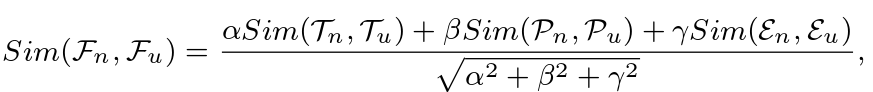
\includegraphics[scale=0.4]{static/figures/sim.png}
    \label{}
\end{figure} 

όπου {\en {\textit{a, b}}} και {\en {\textit{c}}} είναι παράμετροι μέσω των οποίων 
ρυθμίζουμε το πόσο εμπιστευόμαστε τα αντίστοιχα μέρη. 
Στο δικό μας σύστημα συστάσεων επιλέγουμε να αναθέσουμε ίση σημαντικότητα 
σε κάθε έναν από τους παραπάνω παράγοντες, δεδομένου ότι αναπαριστούν διαφορετικές 
αλλά, παράλληλα, συνδεδεμένες πτυχές ενός ειδησεογραφικού άρθρου ή ενός προφίλ χρήστη, 
αναθέτοντας και στους τρεις παράγοντες την ίδια τιμή {\en {\textit{a = b = c = 1}}}. \\

Η {\en {\textit{Sim($T_C, T_U$)}}} υπολογίζεται μέσω της εξίσωσης (2.1), 
ενώ οι {\en {\textit{Sim($P_n, P_u$)}}} και 
{\en {\textit{Sim($E_n, E_u$)}}} 
υπολογίζονται μέσω της ομοιότητας {\en {Jaccard}}. 
Η ομοιότητα {\en {Jaccard}} \cite{Jac02} για δύο σύνολα είναι το μέγεθος της τομής προς το μέγεθος της ένωσής τους. \\

%--------------------------------
\textbf{Εισαγωγή στις {\en {Submodular}} Συναρτήσεις}

Μια κατηγορία συναρτήσεων που χρησιμοποιούνται ευρέως 
και παρουσιάζουν ιδιαίτερο ενδιαφέρον είναι οι {\en {submodular}} συναρτήσεις. 
Οι συναρτήσεις αυτές προσπαθούν να μοντελοποιήσουν το γεγονός ότι 
όσο συνεχίζουμε να δίνουμε αγαθά σε κάποιον χρήστη, 
επέρχεται ένας κορεσμός στην ωφέλειά του. 
Η αύξηση της ωφέλειας από την απόκτηση νέων αγαθών είναι μικρή όταν ο χρήστης έχει ήδη στην κατοχή του κι άλλα αγαθά. 
Έχουμε, λοιπόν, μια μονότονη (φθίνουσα) συμπεριφορά στην αύξηση της ωφέλειας. \\

\textbf{Ορισμός.} Μια συνάρτηση ωφέλειας {\en {f}} για έναν χρήστη {\en {i}} είναι {\en {submodular}} 
αν για οποιαδήποτε δύο υποσύνολα αντικειμένων \textit{{\en {S, T}}}, με \textit{{\en {S}}} $\subseteq$ \textit{{\en {T}}}, 
και για κάθε αντικείμενο \textit{{\en {j}}} $\notin$ \textit{{\en {T}}}, ισχύει ότι 

\begin{figure}[!ht] \centering
    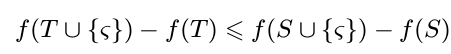
\includegraphics[scale=0.55]{static/figures/modul.png}
    \label{}
\end{figure} 

Ο παραπάνω ορισμός μάς λέει ότι η αύξηση της ωφέλειας που προκαλεί η προσθήκη του αγαθού $\varsigma$ στον χρήστη {\en {i}} 
είναι μεγαλύτερη όταν προσθέτουμε το $\varsigma$ σε ένα σύνολο αγαθών {\en {S}}, από ότι όταν το προσθέτουμε σε ένα 
μεγαλύτερο σύνολο του {\en {S}} (το {\en {T})}. Πάρα πολλά μικροοικονομικά μοντέλα στηρίζονται στην υπόθεση ότι οι 
εμπλεκόμενοι χρήστες έχουν {\en {submodular}} συμπεριφορά. Κλασικό παράδειγμα αποτελούν και τα κοινωνικά δίκτυα, 
όπου η προσθήκη ενός νέου φίλου θα αυξήσει περισσότερο την κοινωνική επιρροή σε μία λιγότερο κοινωνική ομάδα 
από ό,τι σε μία πιο κοινωνική. \\

Μία πιο μαθηματική διατύπωση για το πρόβλημα της μεγιστοποίησης της επιρροής είναι η εξής: 
δεδομένου ενός συνόλου στοιχείων $E$, όπου κάθε στοιχείο είναι συσχετισμένο με μία τιμή επιρροής και ένα κόστος, 
και δεδομένου, επίσης, ενός {\en {budget}} $B$ άρθρων, ο σκοπός είναι να βρεθεί ένα υποσύνολο του $E$ όπου θα 
μεγιστοποιεί την επιρροή (δηλαδή την συνάρτηση {\en {$f(S)$}}) χωρίς το συνολικό κόστος να ξεπερνά το {\en {budget}} $B$. 
Ως {\en {budget}} B μπορεί να θεωρηθεί ο μέγιστος αριθμός από προτεινόμενα άρθρα μέσα σε κάθε {\en {group}} άρθρων. 
Το πρόβλημα της μεγιστοποίησης της επιρροής είναι δυστυχώς {\en {NP-hard}}. 
Ωστόσο, το επιλύουμε μέσω ενός άπληστου {\en {(greedy)}} προσεγγιστικού αλγορίθμου, 
ο οποίος επιλέγει διαδοχικά το στοιχείο το οποίο αυξάνει τη μέγιστη δυνατή επιρροή εντός του ορίου κόστους. 
Δηλαδή προσθέτουμε κάθε φορά στο {\en {S}} το άρθρο που σε αυτό το σημείο μεγιστοποιεί το οριακό κέρδος {\en {(marginal gain)}}.
Ο αλγόριθμος αυτός αποδεικνύεται ότι αποτελεί ($1 - \frac{1}{e})$-προσέγγιση του βέλτιστου, δηλαδή προσέγγιση του βέλτιστου κατά 63\%. \\

\begin{algorithm}
\begin{algorithmic}
 \STATE {\en {Start with an empty set $S$}}
 {\en{
 \FOR {\en{{B iterations}}}
  \STATE {\en {Add article $\varsigma$ to $S$ so that it maximizes $I$($\varsigma$) = $f(S$ $\cup$ \{$\varsigma$\}) - $f(S)$}}
  \ENDFOR }}
\end{algorithmic}
\caption{Άπληστος προσεγγιστικός αλγόριθμος}
\end{algorithm}


%--------------------------------
\textbf{{\en {Submodularity}} Μοντέλο Συστάσεων}

Με βάση τη συγκεκριμένη στρατηγική, ορίζουμε μία συνάρτηση ποιότητας {\en {$f$}} 
για να αξιολογήσουμε το επιλεγμένο σετ άρθρων {\en {$S$}} σε σχέση με ολόκληρο το 
{\en {group}} νέων {\en {$N$}} ως εξής: 

\begin{figure}[!ht] \centering
    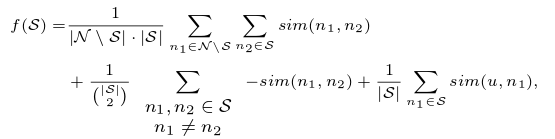
\includegraphics[scale=0.6]{static/figures/quality.png}
    \label{}
\end{figure} 

όπου {\en {$n_1$}} και {\en {$n_2$}} υποδηλώνουν άρθρα, το {\en {$u$}} αναπαριστά 
τον δεδομένο χρήστη και η {\en {$sim(.,.)$}} αναπαριστά την ομοιότητα μεταξύ των δύο προφίλ, 
είτε αναφερόμαστε σε προφίλ χρήστη είτε σε προφίλ άρθρου. \\

Η παραπάνω εξίσωση αποτελείται από τρία μέρη: \\
Το πρώτο στοχεύει στην εκτίμηση της ποιότητας του πόσο αντιπροσωπευτικό είναι το επιλεγμένο σετ νέων $S$, 
το δεύτερο παρέχει μία εικόνα για το πόσο ποικίλα είναι τα θέματα που κρύβονται στα επιλεγμένα άρθρα και τέλος, 
το τρίτο μέρος μάς δίνει στοιχεία για το πόσο ικανοποιούνται οι προτιμήσεις του χρήστη από το επιλεγμένο σετ $S$. 
Η συνάρτηση {\en {$f(S)$}} εξισορροπεί τη συνεισφορά κάθε ενός μέρους. 
Και τα τρία αυτά μέρη αποτελούν {\en {submodular}} συναρτήσεις, άρα είναι μη αρνητικές και μονότονες, 
επομένως και η συνάρτηση {\en {$f(S)$}} θα είναι {\en {submodular}}. \\
Υποθέτοντας ότι το άρθρο $\varsigma$ είναι το υποψήφιο άρθρο, η αύξηση της ωφέλειας αναπαρίσταται ως εξής: 

\begin{figure}[!ht] \centering
    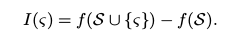
\includegraphics[scale=0.7]{static/figures/increase.png}
    \label{}
\end{figure} 

Στόχος είναι να βρεθεί μία λίστα από άρθρα η οποία μεγιστοποιεί το οριακό κέρδος εντός του δοσμένου {\en {budget}}.
Έτσι, μοντελοποιούμε τις προσωποποιημένες συστάσεις άρθρων ως ένα “προϋπολογισμένο πρόβλημα μέγιστης κάλυψης”. \\

Αρχικά, φροντίζουμε να αφαιρέσουμε από κάθε επιλεγμένο {\en {group}} άρθρων τα άρθρα τα οποία βρίσκονται ήδη 
στο ιστορικό ανάγνωσης του χρήστη, καθώς άρθρα που έχουν ήδη αναγνωσθεί δεν πρέπει να βρεθούν στην τελική προτεινόμενη λίστα. 
Έτσι, καταλήγουμε με μία λίστα από λίστες, κάθε μία εκ των οποίων περιλαμβάνει 
τα εναπομείναντα υποψήφια προς πρόταση άρθρα από κάθε {\en {group}}. \\
Στη συνέχεια, υπολογίζουμε το {\en {budget}} για κάθε λίστα, 
δηλαδή το μέγιστο αριθμό προτεινόμενων άρθρων από κάθε κατηγορία που επιλέχθηκε ως ταιριαστή με τις προτιμήσεις του χρήστη. 
Το {\en {budget}} υπολογίζεται με βάση την ομοιότητα κάθε χρήστη με το εν λόγω {\en {cluster}}/κατηγορία. 
Όσο μεγαλύτερη είναι η τιμή που προκύπτει από τη σύγκριση μεταξύ των κατανομών θεμάτων χρήστη και του εκάστοτε {\en {cluster}}, 
τόσο μεγαλύτερος είναι ο αριθμός άρθρων που επιλέγονται να προταθούν από την εν λόγω κατηγορία άρθρων. \\
Στο σημείο αυτό προβήκαμε σε μία παραδοχή:  
Η εφαρμογή του άπληστου αλγορίθμου {\en {(Algorithm 1)}} σε κάθε {\en {group}} άρθρων (προκειμένου να επιλύσουμε 
το πρόβλημα μέγιστης κάλυψης, επιλέγοντας διαδοχικά το άρθρο που προσφέρει τη μέγιστη αύξηση ωφέλειας από το επιλεγμένο σετ $S$, 
μέσα στο πλαίσιο που ορίζεται από το {\en {budget}}), αποδείχθηκε υπερβολικά χρονοβόρα για ένα τυπικό υπολογιστικό σύστημα 
και ξέφευγε από την ουσία ενός συστήματος συστάσεων. 
Ο χρήστης θα έπρεπε να περιμένει υπερβολικά πολλή ώρα προκειμένου να δεχθεί ως σύσταση τη βέλτιση επιλογή άρθρων, 
όπως θα μας την υποδείκνυε η συνάρτηση αξιολόγησης.
Έτσι, καταφύγαμε στη λύση του να υπολογίσουμε για κάθε {\en {group}} όλους τους δυνατούς συνδυασμούς άρθρων, μεγέθους ίσου με το αντίστοιχο {\en {budget}}, 
και να επιλέξουμε τυχαία έναν από αυτούς μέσω της συνάρτησης {\en {rand}}.
Αν, για παράδειγμα, το {\en {budget}} για ένα {\en {group}} είναι ίσο με την τιμή τρία, τότε υπολογίζουμε όλες τις πιθανές τριάδες άρθρων. \\
Για να ενσωματώσουμε τα προτεινόμενα άρθρα από κάθε {\en {group}} στην τελική προτεινόμενη λίστα, 
επιλέγουμε, λοιπόν, μία τυχαία ν-άδα από κάθε {\en {group}} και όχι απαραίτητα αυτή με την υψηλότερη κατάταξη.
\begin{comment}
Εφαρμόζουμε τον άπληστο αλγόριθμο {\en {(Algorithm 1)}} σε κάθε μία από τις ν-άδες άρθρων 
προκειμένου να επιλύσουμε το πρόβλημα μέγιστης κάλυψης, επιλέγοντας την ν-άδα που προσφέρει τη μέγιστη αύξηση ωφέλειας 
από το επιλεγμένο σετ $S$. \\
Για να ενσωματώσουμε τα προτεινόμενα άρθρα από κάθε {\en {group}} στην τελική προτεινόμενη λίστα, 
επιλέγουμε την ν-άδα με την υψηλότερη κατάταξη από κάθε {\en {group}}.
\end{comment}

\begin{comment}
Εφαρμόζουμε τον άπληστο αλγόριθμο {\en {(Algorithm 1)}} σε κάθε {\en {group}} άρθρων προκειμένου να επιλύσουμε 
το πρόβλημα μέγιστης κάλυψης, επιλέγοντας διαδοχικά το άρθρο που προσφέρει τη μέγιστη αύξηση ωφέλειας από το επιλεγμένο σετ $S$, 
μέσα στο πλαίσιο που ορίζεται από το {\en {budget}}. 
Για να ενσωματώσουμε τα προτεινόμενα άρθρα από κάθε {\en {group}} στην τελική προτεινόμενη λίστα, 
επιλέγουμε τα άρθρα με την υψηλότερη κατάταξη από κάθε {\en {group}}, όπου ο αριθμός των επιλεγμένων άρθρων 
από κάθε {\en {group}} είναι ανάλογος του ενδιαφέροντος του χρήστη για την εν λόγω κατηγορία. \\
\end{comment}

Η {\en {submodularity-based}} στρατηγική επιλογής άρθρων οδηγεί σε μία αρκετά ποικίλη λίστα άρθρων από κάθε κατηγορία. \\
 
%--------------------------------
\textbf{Προσαρμογή Κατάταξης Ειδησεογραφικών Άρθρων} 

Υιοθετώντας τον άπληστο αλγόριθμο που αναλύσαμε νωρίτερα, 
μπορούμε να εξάγουμε μία λίστα από ειδησεογραφικά άρθρα για κάθε θεματική κατηγορία. 
Λαμβάνοντας υπ'όψιν τα αποκλειστικά χαρακτηριστικά των άρθρων, όπως η δημοφιλία και το 
πόσο πρόσφατα δημοσιευμένα είναι, η κατάταξη των επιλεγμένων άρθρων χρειάζεται να προσαρμοστεί 
ώστε να κάνουμε το προτεινόμενο αποτέλεσμα πιο λογικό. \\

Στο σύστημά μας η δημοφιλία ενός άρθρου και το πόσο πρόσφατα δημοσιεύθηκε αποτελούν μέρος του Προφίλ Άρθρου, 
τη δημιουργία του οποίου αναλύσαμε ενδελεχώς σε προηγούμενη παράγραφο. 
Κάνοντας προσαρμογές στη λίστα επιλεγμένων άρθρων, συνδυάζουμε τις κανονικοποιημένες τιμές 
αυτών των δύο τύπων ιδιοτήτων. Τυπικά, δεδομένου ενός άρθρου {\en {$n$}}, 
η δημοφιλία {\en {$n_P$}} και το πόσες μέρες είναι δημοσιευμένο {\en {$n_I$}} 
μπορούν να συνδυαστούν ως εξής: 

\begin{figure}[!ht] \centering
    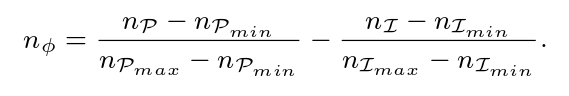
\includegraphics[scale=0.55]{static/figures/comb.png}
    \label{}
\end{figure} 

Παρατηρούμε ότι όσο πιο πρόσφατα δημοσιεύθηκε ένα άρθρο 
(και άρα, όσο πιο μικρή η τιμή του εν λόγω χαρακτηριστικού), 
τόσο υψηλότερη θέση παίρνει το άρθρο στην τελική κατάταξη. 
Δεδομένης μια λίστας άρθρων προς σύσταση, επιλέγουμε διαδοχικά 
δύο γειτονικά άρθρα {\en {$n_i$}} και {\en {$n_j$}} από την κορυφή της λίστας προς τα κάτω 
και τα συγκρίνουμε ως προς το δυναμικό τους σκορ, {\en {$n_f$}}. 
Εάν η εν λόγω διαφορά είναι μεγαλύτερη από μηδέν, ανταλλάσουμε τη θέση των δύο αυτών άρθρων. 
Αλλιώς, τα προσπερνούμε και συνεχίζουμε με τη σύγκριση του επόμενου ζεύγους άρθρων. \\

Μέσω αυτής της μικρής προσαρμογής η παραγόμενη κατάταξη δίνει έμφαση στα πιο δημοφιλή και 
“φρέσκα” ειδησεογραφικά άρθρα, καθώς, επίσης, επικεντρώνεται σε άρθρα που ικανοποιούν σε 
μεγαλύτερο βαθμό τις αναγνωστικές προτιμήσεις του χρήστη. 














	\chapter{\selectlanguage{greek}Τεχνολογίες Υλοποίησης}

Στο κεφάλαιο αυτό θα περιγράψουμε τα εργαλεία και τις τεχνολογίες που χρησιμοποιήθηκαν για την υλοποίησή μας. \\

\section{Η γλώσσα προγραμματισμού \en {Python}}

Η γλώσσα προγραμματισμού {\en {Python}} \cite{Py02}, \cite{Py01} είναι μια γλώσσα διερμηνευόμενη και {\en {object-oriented}}. 
Η σύλληψη της {\en {Python}} έγινε στα τέλη της δεκαετίας του 1980 και η εφαρμογή της έγινε το Δεκέμβριο του 1989 από τον Ολλανδό {\en {Guido Van Rossum}}, 
ο οποίος είναι και ο κύριος συγγραφέας της. Το όνομα της γλώσσας προέρχεται από την ομάδα Άγγλων κωμικών {\en {Monty Python}}.
O κώδικάς της διανέμεται με την άδεια {\en {Python Software Foundation}}. 
Ανάμεσα στα κύρια χαρακτηριστικά της είναι τα εξής: γλώσσα ανοιχτού κώδικα {\en {(open source)}}, αναγνωσιμότητα, εύκολη εκμάθηση, 
επεκτασιμότητα, εύκολη συντήρηση, δυνατότητα απλοποίησης στην υλοποίηση δύσκολων συναρτήσεων, γρήγορη ανάπτυξη εφαρμογών.

\par Η ίδια η γλώσσα είναι επεκτάσιμη καθώς ένα βασικό σύνολο της γλώσσας αποτελεί τον πυρήνα της, 
ενώ όλα τα υπόλοιπα είναι βιβλιοθήκες {\en {(modules)}} που επεκτείνουν την λειτουργικότητά της. 
Oι κύριοι τύποι δεδομένων που χρησιμοποιεί είναι οι λίστες, τα λεξικά και οι πλειάδες. 
Έχει μεγαλο εύρος εφαρμογών, όπως για παράδειγμα στον επιστημονικό υπολογισμό, στην τεχνητή νοημοσύνη, 
στην επεξεργασία φυσικής γλώσσας κλπ.

\par Στην παρούσα διπλωματική εργασία χρησιμοποιήσαμε την έκδοση 3.4.0 της γλώσσας, 
η οποία σε συνδυασμό με την πλατφόρμα {\en {NLTK}} χρησιμεύουν σε πολλές εφαρμογές της επεξεργασίας φυσικής γλώσσας.

\section{\en{MySQL}}

Η {\en {MySQL}} \cite{sql01} είναι ένα ανοιχτού λογισμικού σύστημα διαχείρισης σχεσιακών βάσεων δεδομένων. 
Η ονομασία {\en {MySQL}} περιέχει δύο στοιχεία: το {\en {My}}  είναι το όνομα της κόρης του συνιδρυτή του συστήματος, {\en {Monty Widenius}} 
και το {\en {SQL}} αναφέρεται στη γλώσσα {\en {SQL (Structured Query Language)}}, 
μια γλώσσα υπολογιστών που αναπτύχθηκε ξεχωριστά από τις υλοποιήσεις συστημάτων διαχείρισης βάσεων δεδομένων 
(όπως της {\en {MySQL}}, της {\en {PostgreSQL}}, της {\en {Oracle}} κλπ).
Το πρόγραμμα τρέχει έναν εξυπηρετητή {\en {(server)}} παρέχοντας πρόσβαση πολλών χρηστών σε ένα σύνολο βάσεων δεδομένων.
Tο λογισμικό αυτό επιτρέπει στους χρήστες να δημιουργούν και να χρησιμοποιούν μια βάση δεδομένων, παρέχοντάς τους δυνατότητες όπως
ο ορισμός, η κατασκευή, η χρήση/προσπέλαση και η διαγραφή αυτής.
\par Θα μπορούσαμε να υλοποιήσουμε μια βάση δεδομένων και χωρίς τη χρήση συστήματος διαχείρισης (πχ. με χρήση αρχείων).
Τα σημαντικότερα πλεονεκτήματα του συστήματος διαχείρισης είναι η ευκολία στη σχεδίαση και την υλοποίηση, 
η γρήγορη ανάπτυξη εφαρμογών, η ακεραιότητα των δεδομένων, ο έλεγχος πρόσβασης χρηστών, η ταυτόχρονη χρήση από πολλούς χρήστες, 
ο έλεγχος ορθότητας/πλεονασμών και οι έτοιμες συναρτήσεις/αλγόριθμοι.

\par Η {\en {MySQL}} χρησιμοποιείται ευραίως σε διάφορες εφαρμογές όπως οι {\en {TYPO3, Joomla, Wordpress, phpBB, MyBB, Drupal}}.
Χρησιμοποιείται επίσης και σε κάποιες από τις πιο διαδεδομένες διαδικτυακές υπηρεσίες, όπως το {\en {Flickr}}, το {\en {YouTube}}, η {\en {Wikipedia}}, 
το {\en {Google}}, το {\en {Facebook}} και το {\en {Twitter}}.

\par Στην παρούσα διπλωματική εργασία χρησιμοποιήσαμε την έκδοση 5.6.33.

\section{\en{HTML}}

Η {\en{HTML}} (αρχικοποίηση του αγγλικού {\en {HyperText Markup Language}} \cite{Ht01}, ελλ. Γλώσσα Σήμανσης Υπερκειμένου) είναι η κύρια γλώσσα σήμανσης για τις ιστοσελίδες, 
και τα στοιχεία της είναι τα βασικά δομικά στοιχεία των ιστοσελίδων.

Η {\en{HTML}} γράφεται υπό μορφή στοιχείων {\en{HTML}} τα οποία αποτελούνται από ετικέτες {\en {(tags)}}, 
οι οποίες περικλείονται μέσα σε σύμβολα «μεγαλύτερο από» και «μικρότερο από», μέσα στο περιεχόμενο της ιστοσελίδας. 
Οι ετικέτες {\en{HTML}} συνήθως λειτουργούν ανά ζεύγη, 
με την πρώτη να ονομάζεται ετικέτα έναρξης και τη δεύτερη ετικέτα λήξης 
(ή σε άλλες περιπτώσεις ετικέτα ανοίγματος και ετικέτα κλεισίματος αντίστοιχα). 
Ανάμεσα στις ετικέτες οι σχεδιαστές ιστοσελίδων μπορούν να τοποθετήσουν κείμενο, πίνακες, εικόνες κλπ.

\par Ο σκοπός ενός {\en {web browser}} είναι να διαβάζει τα έγγραφα {\en{HTML}} και τα συνθέτει σε σελίδες που μπορεί κανείς να διαβάσει ή να ακούσει. 
Ο {\en {browser}} δεν εμφανίζει τις ετικέτες {\en{HTML}}, αλλά τις χρησιμοποιεί για να ερμηνεύσει το περιεχόμενο της σελίδας.

\par Τα στοιχεία της {\en{HTML}} χρησιμοποιούνται για να κτίσουν όλους τους ιστότοπους. 
Η {\en{HTML}} επιτρέπει την ενσωμάτωση εικόνων και άλλων αντικειμένων μέσα στη σελίδα 
και μπορεί να χρησιμοποιηθεί για να εμφανίσει διαδραστικές φόρμες. 
Παρέχει τις μεθόδους δημιουργίας δομημένων εγγράφων (δηλαδή εγγράφων που αποτελούνται από το περιεχόμενο που μεταφέρουν 
και από τον κώδικα μορφοποίησης του περιεχομένου) καθορίζοντας δομικά σημαντικά στοιχεία για το κείμενο, 
όπως κεφαλίδες, παραγράφους, λίστες, συνδέσμους, παραθέσεις και άλλα. 
Μπορούν, επίσης, να ενσωματώνονται σενάρια εντολών σε γλώσσες όπως η {\en {JavaScript}}, 
τα οποία επηρεάζουν τη συμπεριφορά των ιστοσελίδων {\en{HTML}}.

\par Οι {\en {Web browsers}} μπορούν επίσης να αναφέρονται σε στυλ μορφοποίησης {\en {CSS}} 
για να ορίζουν την εμφάνιση και τη διάταξη του κειμένου και του υπόλοιπου υλικού. 
Ο οργανισμός {\en {W3C}}, ο οποίος δημιουργεί και συντηρεί τα πρότυπα για την {\en{HTML}} και τα {\en {CSS}}, 
ενθαρρύνει τη χρήση των {\en {CSS}} αντί διαφόρων στοιχείων της {\en {HTML}} για σκοπούς παρουσίασης του περιεχομένου.

\section{\en{CSS}}

Η {\en {CSS (Cascading Style Sheets}} \cite{w3css} - Διαδοχικά Φύλλα Στυλ ή αλληλουχία
φύλλων στυλ) είναι μια γλώσσα υπολογιστή που ανήκει στην κατηγορία των
γλωσσών φύλλων στυλ που χρησιμοποιείται για τον έλεγχο της εμφάνισης
ενός εγγράφου που έχει γραφτεί με μια γλώσσα σήμανσης. Χρησιμοποιείται
δηλαδή για τον έλεγχο της εμφάνισης ενός εγγράφου που γράφτηκε στις
γλώσσες {\en {HTML}} και {\en {XHTML}}, δηλαδή για τον έλεγχο της εμφάνισης μιας
ιστοσελίδας και γενικότερα ενός ιστοτόπου.
Η {\en {CSS}} είναι μια γλώσσα υπολογιστή προορισμένη να αναπτύσσει στυλιστικά μια ιστοσελίδα, 
δηλαδή να διαμορφώνει περισσότερα χαρακτηριστικά, χρώμματα, στοίχιση και δίνει περισσότερες δυνατότητες σε σχέση με την {\en {html}}.
Η χρήση της {\en {CSS}} κρίνεται ως απαραίτητη για μια όμορφη και καλοσχεδιασμένη ιστοσελίδα .

\section{\en {Apache HTTP Server}}

Ο {\en {Apache HTTP Server}} \cite{Ap01}, γνωστός και απλά σαν {\en {Apache}}, είναι ένας εξυπηρετητής του παγκόσμιου ιστού {\en {(web)}}. 
Όποτε ένας χρήστης επισκέπτεται έναν ιστότοπο, το πρόγραμμα πλοήγησης {\en {(browser)}} επικοινωνεί με έναν διακομιστή {\en {(server)}} 
μέσω του πρωτοκόλλου {\en {HTTP}}, ο οποίος παράγει τις ιστοσελίδες και τις αποστέλλει στο πρόγραμμα πλοήγησης. 
Κυκλοφόρησε υπό την άδεια λογισμικού {\en {Apache}} και είναι λογισμικό ανοιχτού κώδικα.

\par Ο {\en {Apache}} χρησιμοποιείται και σε τοπικά δίκτυα σαν διακομιστής συνεργαζόμενος με συστήματα διαχείρισης Βάσης Δεδομένων, π.χ. {\en {MySQL}},
όπως και χρησιμοποιήθηκε στην παρούσα διπλωματική (έκδοση 2.4.7).

\section{\en{Flask Web Framework}}

Τα {\en {Web Frameworks} είναι σχεδιασμένα για να υποστηρίζουν την ανάπτυξη διαδικτυακών εφαρμογών. 
Κάθε εφαρμογή που απαιτεί τη χρήση βάσεων δεδομένων, φορμών, συνόδων {\en {(sessions), cookies} 
ή κάποιας απομακρυσμένης υπηρεσίας (όπως είναι το {\en {Twitter}}, το {\en {Facebook}} κλπ) θα ωφεληθεί αν υλοποιηθεί με κάποιο {\en {Framework}}.

\par Το {\en {Flask}} \cite{Fl01} είναι ένα {\en {micro web framework}} γραμμένο σε {\en {Python}}.

\section{Εργαλεία Επεξεργασίας Φυσικής Γλώσσας}

\subsection{\en {Tree Tagger}}
Ο {\en {Tree Tagger}} \cite{Tt01} είναι ένα εργαλείο που δημιουργήθηκε από τον {\en {Helmud
Schmid}} στο Ινστιτούτο για τον γλωσσικό υπολογισμό στο Πανεπιστήμιο της Στουτγκάρδης. 
Αποτελείται από ένα εργαλείο για σχολιασμό κειμένου με βάση το σε τι μέρος του λόγου αντιστοιχίζεται η κάθε λέξη,
καθώς και πληροφορία για λήμματα. Ο {\en {Tree Tagger}} δουλεύει πολύ καλά για την Αγγλική γλώσσα,
αλλά υποστηρίζει επίσης και άλλες γλώσσες όπως Ισπανικά, Γαλλικά, Ιταλικά, Ολλανδικά, Βουλγαρικά, Ρωσικά, Ελληνικά, Πορτογαλικά κ.λπ.
Ο {\en {Tree Tagger}} περιλαμβάνει κατηγορίες στις οποίες ανήκουν οι λέξεις. Οι
κατηγορίες αυτές αντιπροσωπεύουν στην ουσία τα μέρη του λόγου μιας
πρότασης. Ένα παράδειγμα μιας τέτοιας κατηγορίας είναι το NN, το οποίο
υποδηλώνει ουσιαστικό. 
Παρακάτω ακολουθεί ένας αναλυτικός πίνακας με τις κατηγορίες του {\en {Tree Tagger}} και τι σημαίνει η καθεμία.

\begin{figure}[!ht] \centering
	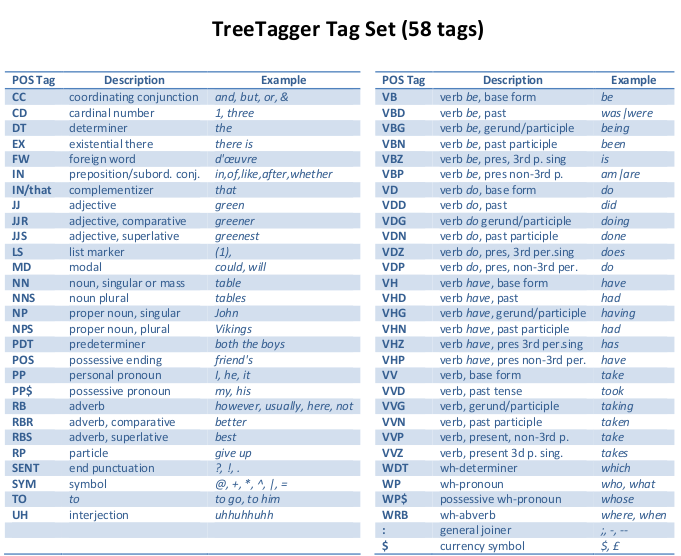
\includegraphics[scale=0.65]{static/figures/treetagger.png}
    \caption{Κατηγορίες {\en {Tree Tagger.}}}
    \label{}
\end{figure} 

\subsection{\en {NLTK}}
Το {\en {NLTK (Natural Language Toolkit)}} \cite{Nl02} είναι ένα πακέτο βιβλιοθηκών και προγραμμάτων της {\en {Python}} 
για εφαρμογές της Επεξεργασίας Φυσικής Γλώσσας και αναπτύχθηκε απ’τους
{\en {Steven  Bird,  Edward  Loper}} και {\en {Ewan  Klein}}.
Περιλαμβάνει πολλά γνωστά σώματα κειμένων, γραφικές αναπαραστάσεις
και δειγματικά δεδομένα. Συνοδεύεται από ένα βιβλίο το οποίο εξηγεί τις
έννοιες που σχετίζονται με τα εργαλεία που παρέχει. 
Βασικός στόχος του {\en {NLTK}} είναι να υποστηρίξει την έρευνα και την εκμάθηση της Επεξεργασίας
Φυσικής Γλώσσας καθώς και άλλων σχετικών πεδίων, όπως η Γλωσσολογία,
η Τεχνητή Νοημοσύνη, η Ανάκτηση Πληροφορίας και η Μηχανική Μάθηση. 
Όταν λέμε φυσική γλώσσα εννοούμε μια γλώσσα η οποία χρησιμοποιείται για την καθημερινή
επικοινωνία των ανθρώπων. Σε αντίθεση με τις τεχνητές γλώσσες, όπως οι γλώσσες προγραμματισμού
και η μαθηματική σημειογραφία, οι φυσικές γλώσσες έχουν εξελιχθεί καθώς
περνούν από γενιά σε γενιά και είναι αρκετά δύσκολο να μπορέσουν να
οριστούν με ρητούς κανόνες. 
'Εχει χρησιμοποιηθεί με επιτυχία ως εργαλείο διδασκαλίας, μελέτης και ως
πλατφόρμα για την ανάπτυξη πρωτότυπων ερευνητικών συστημάτων. \\

Το {\en {NLTK}} δημιουργήθηκε με βάση τέσσερις πρωταρχικούς σκοπούς:
\begin{itemize}
 \item \textbf{Απλότητα {\en {(Simplicity)}}}: Το να παρέχεται ένα διαισθητικό πλαίσιο εργασίας παράλληλα με ουσιώδεις
οικοδομικούς λίθους, δίνοντας στους χρήστες μια πρακτική γνώση της φυσικής επεξεργασίας γλώσσας 
χωρίς να βαλτώνουν στη βαρέτη εργασία της επεξεργασίας σχολιασμένων γλωσσικών δεδομένων.
 \item \textbf{Συνέπεια {\en {(Consistency)}}}: Το να παρέχεται ένα αμετάβλητο πλαίσιο εργασίας με συνεπείς διεπαφές και
δομές δεδομένων και εύκολα προβλέψιμα ονόματα μεθόδων.
 \item \textbf{Επεκτασιμότητα {\en {(Extensibility)}}}: Το να παρέχεται μια δομή μέσα στην οποία νέες υπομονάδες λογισμικού
μπορούν εύκολα να φιλοξενηθούν, περιλαμβάνοντας διαφορετικές υλοποιήσεις 
και περιλαμβάνοντας συναγωνιστικές προσεγγίσεις στην ίδια αποστολή.
 \item \textbf{Συναρμολογισιμότητα {\en {(Modularity)}}}: Το να παρέχονται συστατικά που μπορούν να χρησιμοποιηθούν ανεξάρτητα
χωρίς την ανάγκη κατανόησης του υπόλοιπου πακέτου.\newline
\end{itemize}

Κατά την υλοποίηση του συστήματός μας χρησιμοποιήσαμε την έκδοση 3.2.1 του {\en {NLTK}} για τις παρακάτω διαδικασίες:
\begin{itemize}
  \item \textbf{Χωρισμός του κειμένου σε προτάσεις {\en {(Sentence Tokenization/Segmentation).}}}\\
Αν θέλουμε να χωρίσουμε σε προτάσεις ένα κομμάτι κειμένου, τότε μπορούμε να ακολουθήσουμε την παρακάτω διαδικασία:
\begin{figure}[!ht] \centering
    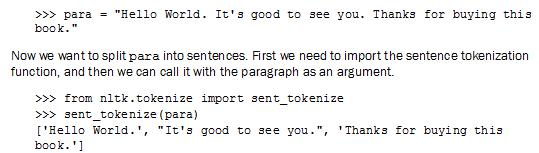
\includegraphics[scale=0.7]{static/figures/nltk1.png}
    \caption{Χωρισμός προτάσεων.}
    \label{}
\end{figure}
\\ Έτσι, τώρα έχουμε μια λίστα με τις προτάσεις και μπορούμε να τις χρησιμοποιήσουμε για περαιτέρω επεξεργασία. 

  \item \textbf{Χωρισμός των προτάσεων σε λέξεις {\en {(Word Tokenization).}}}\\
Αν θέλουμε να διαχωρίσουμε μια πρόταση σε μεμονωμένες λέξεις, θα ακολουθήσουμε τη διαδικασία που φαίνεται στην εικόνα:
\begin{figure}[!ht] \centering
    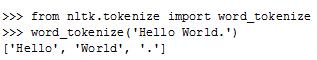
\includegraphics[scale=0.75]{static/figures/nltk3.png}
    \caption{Χωρισμός προτάσεων σε λέξεις.}
    \label{}
\end{figure}

\item \textbf{Απομάκρυνση ανεπιθύμητων λέξεων {\en {(Removing Stopwords).}}}\\
\begin{comment}
\begin{figure}[!ht] \centering
    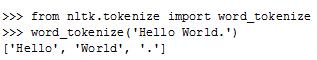
\includegraphics[scale=0.75]{static/figures/nltk3.png}
    \caption{Απομάκρυνση ανεπιθύμητων λέξεων.}
    \label{}
\end{figure}
\end{comment}
\end{itemize}

\subsection{\en {GATE for Named Entity Recognition}}
%Το σύστημα, αφού αναγνωρίσει μια ονοματισμένη οντότητα (π.χ. πρόσωπο, οργανισμό, εταιρεία κτλ.)...

Το {\en {GATE (General Architecture for Text Engineering)}} \cite{Gt01} αποτελεί πλατφόρμα ανοιχτού κώδικα για την επεξεργασία και ανάλυση κειμένων φυσικής γλώσσας, 
παρέχοντας εργαλεία ανάλυσης κειμένου. Το {\en {GATE}} διανέμεται με το σύστημα διεξαγωγής πληροφοριών γνωστό ως {\en {ANNIE}}, 
το οποίο έχει αποτελέσει τη βάση πολλών εμπορικών και ερευνητικών συστημάτων.
Το {\en {ANNIE}} είναι σε θέση να αναγνωρίσει έναν αριθμό διαφορετικών τύπων οντοτήτων, όπως ονόματα, τοποθεσίες και οργανισμούς, 
απαντώντας έτσι σε ερωτήσεις όπως “Τι συνέβη, ποιος εμπλέκεται, πότε συνέβη” κ.λπ, φράσεις οι οποίες 
ενδέχεται να κεντρίζουν το ενδιαφέρον αρκετών χρηστών ως προς την επιλογή άρθρων προς ανάγνωση. \\

\begin{figure}[!ht] \centering
\centerline{
    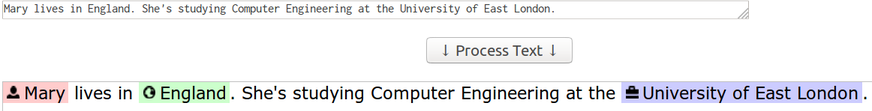
\includegraphics[scale=0.5]{static/figures/gate.png}}
    \caption{Αναγνώριση ονοματισμένων οντοτήτων.}
    \label{}
\end{figure}

\newpage

\begin{figure}[!ht] \centering
\centerline{
    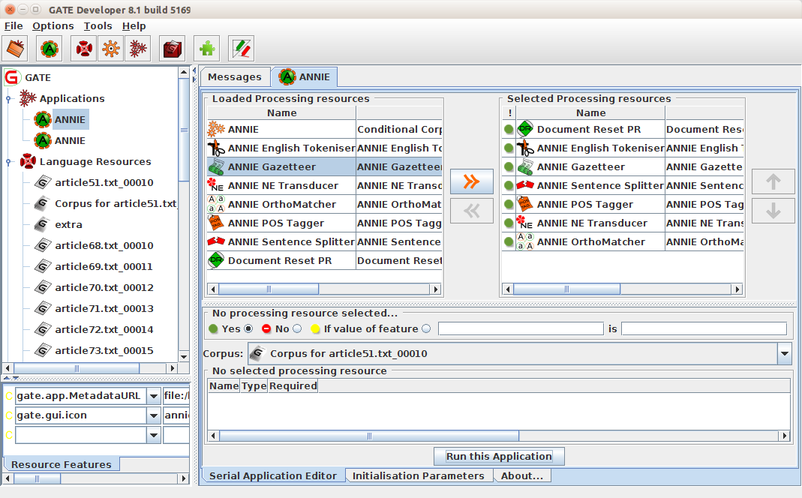
\includegraphics[scale=0.5]{static/figures/gate1.png}}
    \caption{Εφαρμογή του εργαλείου {\en {ANNIE Gazetteer}} στο {\en {corpus}} κειμένων.}
    \label{}
\end{figure}

\begin{figure}[!ht] \centering
\centerline{
    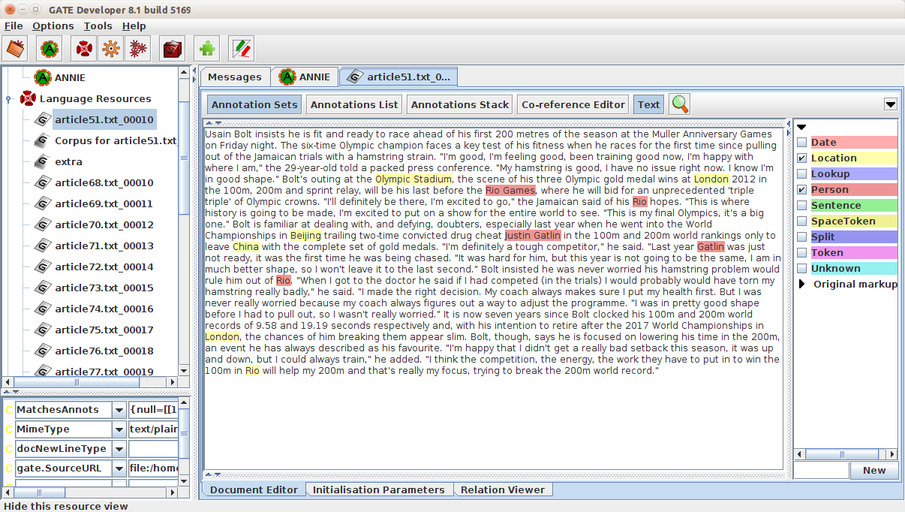
\includegraphics[scale=0.45]{static/figures/gate2.png}}
    \caption{Επιλογή των ετικετών που μας ενδιαφέρουν μέσω της δεξιάς στήλης.}
    \label{}
\end{figure}











	\chapter{{\en {PELOMA: A Personalized News Recommendation System}}}

Στην ενότητα αυτή θα παρουσιάσουμε την διεπαφή χρήστη. 
Η διεπαφή αποτελεί έναν σημαντικό διαμεσολαβητή μεταξύ συστήματος και χρήστη. 
Μέσω της διεπαφής ο χρήστης έχει την δυνατότητα να επικοινωνήσει με το σύστημα, 
δηλαδή να δώσει τα δεδομένα του σε αυτό και να πάρει αποτελέσματα από αυτό. \\

Για να μπορέσει να λειτουργήσει η εφαρμογή θα πρέπει να εκτελεστούν μια φορά τα απαραίτητα
υποσυστήματα, η λειτουργία των οποίων έχει αναλυθεί εκτενώς στο Κεφάλαιο 2:

\begin{itemize}
\item \textbf{Υποσύστημα Δημιουργίας Βάσης Δεδομένων και Καταχώρησης Πληροφορίας} \\
Το υποσύστημα αυτό θα δημιουργήσει τη βάση δεδομένων και θα καταχωρήσει την απαραίτητη 
για τα επόμενα υποσυστήματα πληροφορία σχετικά με τα άρθρα. 

\item \textbf{Υποσύστημα Ομαδοποίησης Ειδησεογραφικών Άρθρων} \\
Στο υποσύστημα αυτό προβαίνουμε σε ομαδοποίηση των ειδησεογραφικών άρθρων που βρίσκονται 
αποθηκευμένα στη βάση δεδομένων σε κατηγορίες {\en {(clusters)}}, 
ομαδοποίηση των ειδησεογραφικών άρθρων εντός των {\en {clusters}} σε ομάδες {\en {(groups)}}, 
καθώς και σε εντοπισμό ειδησεογραφικών θεμάτων μέσω πιθανοτικών μοντέλων θεμάτων 
για κάθε {\en {cluster, group}} και μεμονωμένο άρθρο της συλλογής. 
Επιπρόσθετα, κάνουμε εξαγωγή ονοματισμένων οντοτήτων για κάθε άρθρο.
Όλη η παραχθείσα νέα πληροφορία αποθηκεύεται στη βάση δεδομένων. 
\end{itemize}

\newpage
Παρακάτω παρουσίαζουμε το περιβάλλον της διεπαφής: \\

\begin{figure}[!ht] \centering
\centerline{
    
\includegraphics[scale=0.45]{static/figures/peloma/start.png}}
    \caption{Αρχική εικόνα περιβάλλοντος διεπαφής.}
    \label{}
\end{figure} 

\begin{figure}[!ht] \centering
\centerline{
    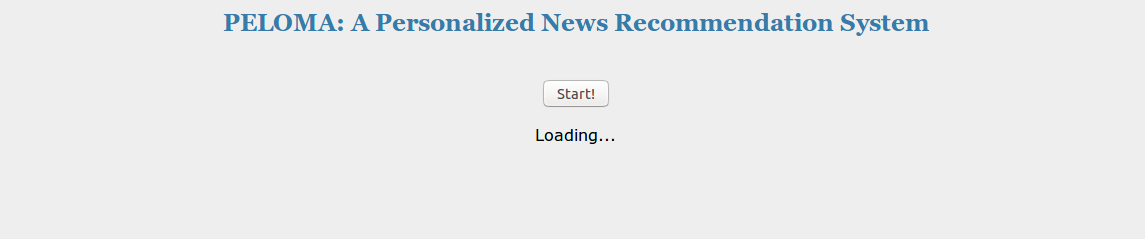
\includegraphics[scale=0.46]{static/figures/peloma/loading.png}}
    \caption{Αναμονή για δημιουργία προφίλ αποθηκευμένων χρηστών και άρθρων.}
    \label{}
\end{figure} 

% Όπως έχουμε αναφέρει, κατά τη δημιουργία της βάσης δεδομένων καταχωρήσαμε και μία λίστα χρηστών μαζί με το αναγνωστικό τους ιστορικό. \\
Αρχικά, μέσω του κουμπιού {\en {Start!}} δημιουργούμε κάποια έτοιμα προφίλ, 
τόσο για τους αποθηκευμένους χρήστες, όσο και για τα άρθρα που βρίσκονται στο ιστορικό τους, 
πριν επιτρέψουμε σε ένα νέο χρήστη να εισέλθει στο σύστημα. 
Η αναγκαιότητα δημιουργίας έτοιμων προφίλ χρηστών προκύπτει από την απαίτηση του συστήματος για εμπλουτισμό 
κάθε προφίλ χρήστη με μία λίστα από άλλους χρήστες του συστήματος που επιδεικνύουν παρόμοια αναγνωστική συμπεριφορά. \\
Στο στάδιο αυτό υπολογίζονται και καταχωρούνται για κάθε άρθρο του ιστορικού των αποθηκευμένων χρηστών 
τόσο στατικά χαρακτηριστικά (π.χ. ονοματισμένες οντότητες), 
όσο και δυναμικά χαρακτηριστικά (π.χ. χρήστες που το διάβασαν, δημοφιλία, 
πόσο “φρέσκο” είναι από τη σκοπιά του πόσο πρόσφατα δημοσιεύθηκε).\\
Επιπρόσθετα, υπολογίζονται η κατανομή των θεμάτων των ειδησεογραφικών άρθρων 
τα οποία ο κάθε αποθηκευμένος χρήστης έχει διαβάσει στο παρελθόν, 
η ομοιότητά του με άλλους αποθηκευμένους χρήστες, καθώς και οι ονοματισμένες οντότητες των άρθρων του ιστορικού του.  \\

\newpage
Στο επόμενο βήμα πραγματοποιείται η είσοδος του χρήστη στο σύστημα μέσω της φόρμας της εικόνας \ref{fig:inter01}. 
Μπορούμε είτε να επιλέξουμε το {\en {username}} ενός από τους ήδη αποθηκευμένους χρήστες 
κάνοντας χρήση του {\en {drop-down list}} που εμφανίζεται και επιλέγοντας ένα από τα ονόματα της λίστας, 
είτε να δημιουργήσουμε έναν νέο χρήστη εισάγοντας το επιθυμητό {\en {username}} στο κενό πεδίο της φόρμας. \\

\begin{figure}[!ht] \centering
\centerline{
    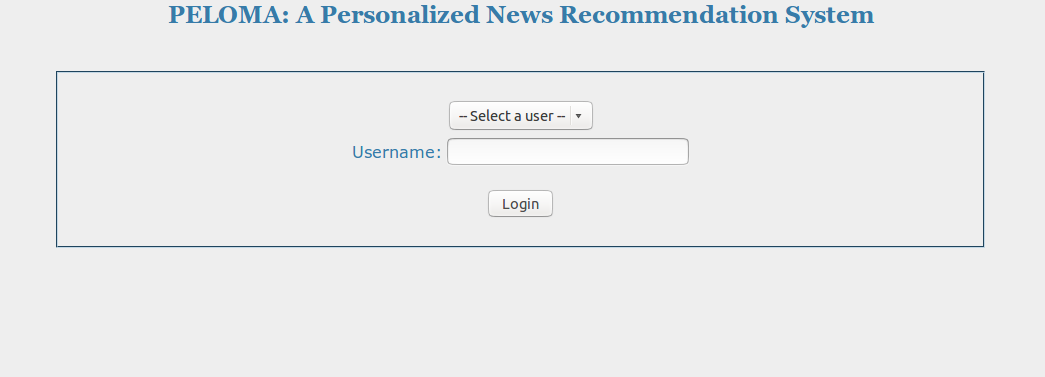
\includegraphics[scale=0.5]{static/figures/peloma/login.png}}
    \caption{Είσοδος χρήστη στο σύστημα.}
    \label{fig:inter01}
\end{figure} 

\begin{figure}[!ht] \centering
\centerline{
    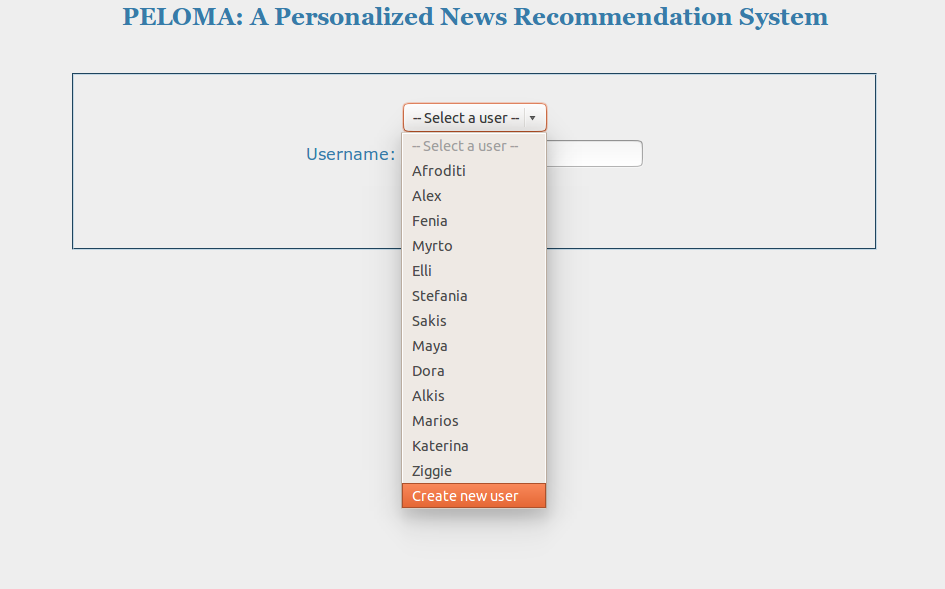
\includegraphics[scale=0.47]{static/figures/peloma/login2.png}}
    \caption{Είσοδος χρήστη στο σύστημα.}
    \label{}
\end{figure} 

Αμέσως μετά τη σύνδεση στο σύστημα, ο χρήστης οδηγείται στην κεντρική σελίδα της εφαρμογής, 
μέσω της οποίας αποκτά πρόσβαση στα άρθρα που είναι αποθηκευμένα στη βάση δεδομένων. 
Στην επάνω δεξιά γωνία του συστήματος αναγράφεται το {\en {username}} του συνδεδεμένου χρήστη και 
παρέχεται κουμπί για την αποσύνδεσή του από το σύστημα. 
Κατά την αποσύνδεση, ο χρήστης οδηγείται στην αρχική φόρμα εισόδου στην εφαρμογή. \\

\begin{figure}[!ht] \centering
\centerline{
    
\includegraphics[scale=0.35]{static/figures/peloma/logout.png}}
    \caption{Κουμπί αποσύνδεσης από το σύστημα.}
    \label{}
\end{figure} 

Σε περίπτωση όπου ο χρήστης επιχειρήσει τη λήψη συστάσεων χωρίς να έχει διαβάσει κάποιο από τα άρθρα του συστήματος, 
εμφανίζεται σχετικό μήνυμα, ενημερώνοντάς τον πως πρέπει να διαβάσει τουλάχιστον ένα άρθρο από κάποια κατηγορία 
προκειμένου να δωθεί στο σύστημα η απαραίτητη είσοδος σχετικά με τις προτιμήσεις του. \\

\begin{figure}[!ht] \centering
\centerline{
    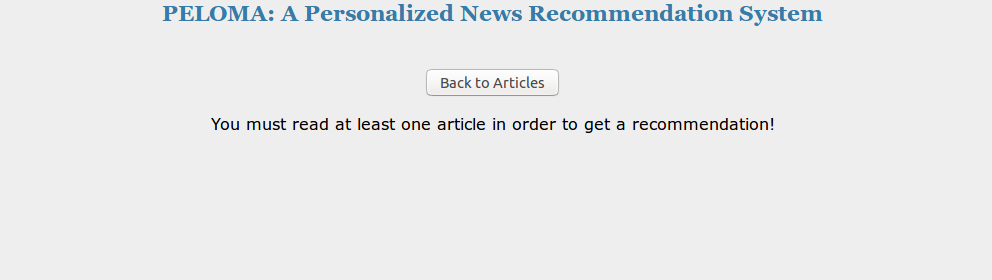
\includegraphics[scale=0.5]{static/figures/peloma/not.png}}
    \caption{Προσπάθεια λήψης συστάσεων πριν την ανάγνωση άρθρων.}
    \label{}
\end{figure} 

\newpage

Τα άρθρα παρουσιάζονται μέσω μιας λίστας στην οποία αναγράφονται το {\en {id}} της κατηγορίας, το {\en {id}} και ο τίτλος του κάθε άρθρου, 
ο οποίος τίτλος αποτελεί και {\en {link}} προς το πλήρες κείμενο. \\

\begin{figure}[!ht] \centering
\centerline{
    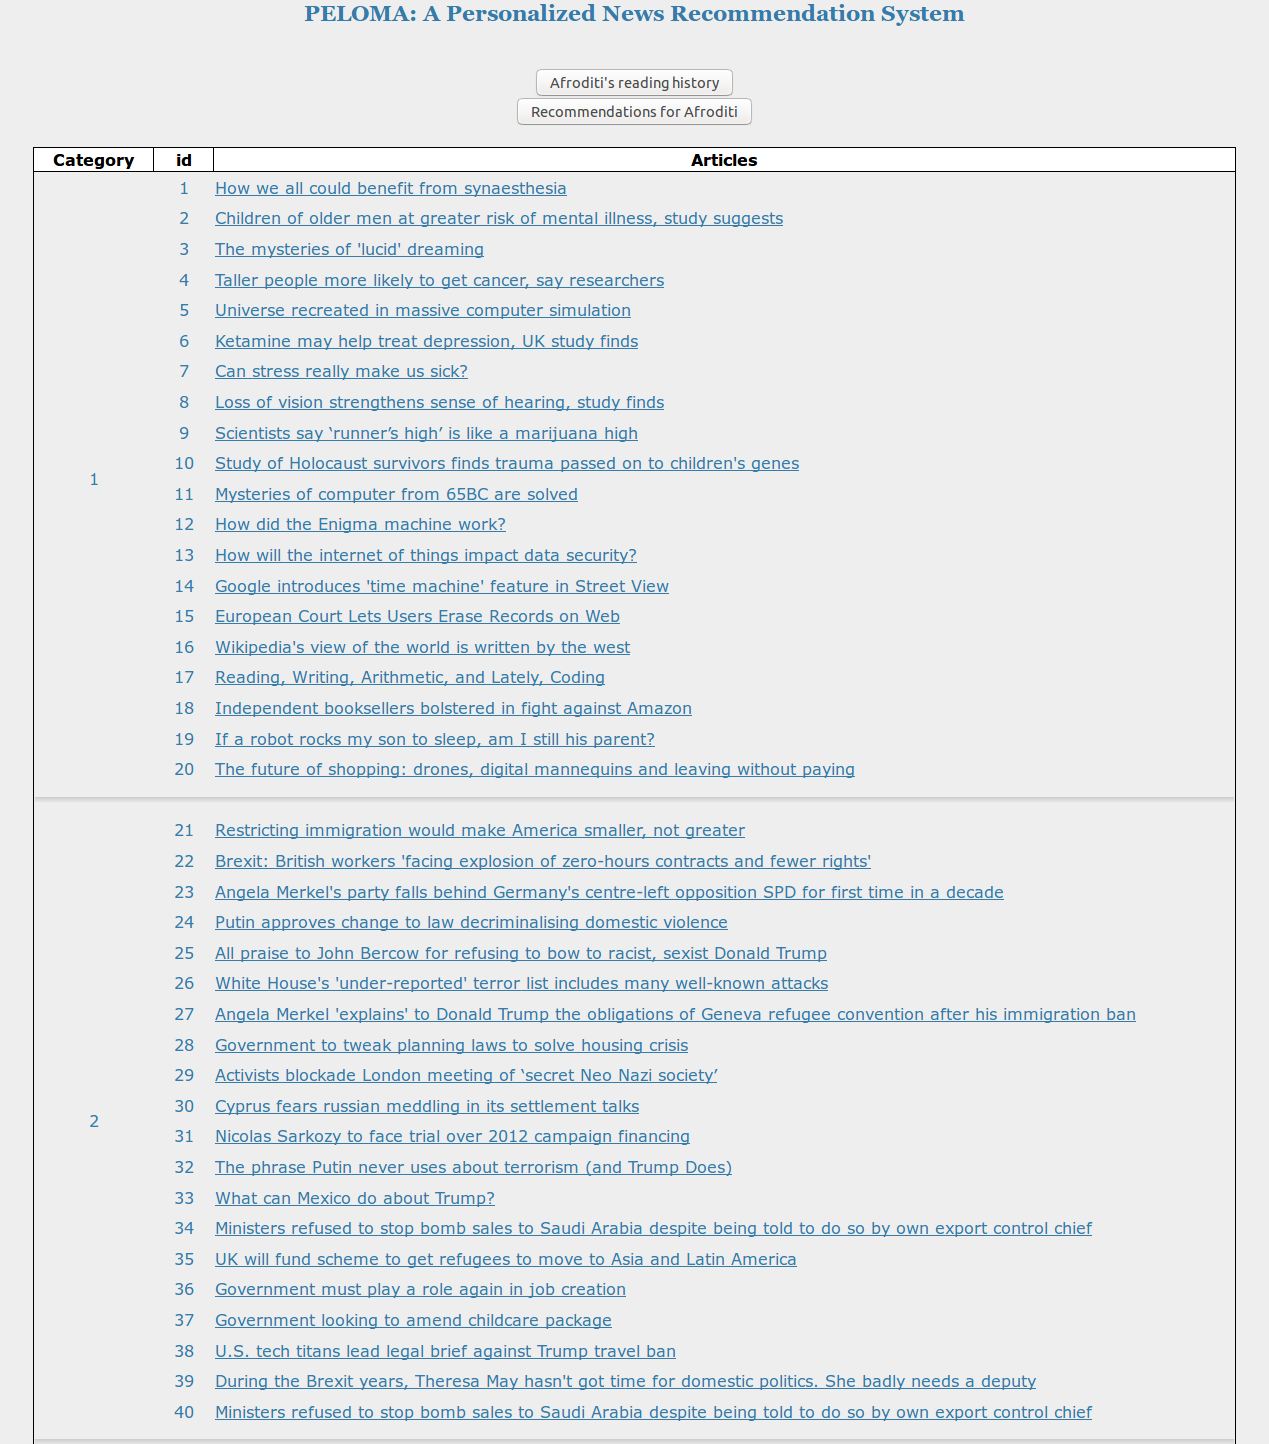
\includegraphics[scale=0.38]{static/figures/peloma/articles.png}}
    \caption{Προβολή λίστας άρθρων βάσης δεδομένων.}
    \label{}
\end{figure} 

\newpage

Παρακάτω βλέπουμε τη μορφή με την οποία παρουσιάζεται στο χρήστη το πλήρες κείμενο ενός άρθρου. 
Κατά το τέλος της ανάγνωσης ο χρήστης μπορεί να επιστρέψει στην αρχική λίστα άρθρων 
κάνοντας χρήση του κουμπιού \textit{{\en {Back to Articles}}} που βρίσκεται στο επάνω μέρος της σελίδας. \\

\begin{figure}[!ht] \centering
\centerline{
    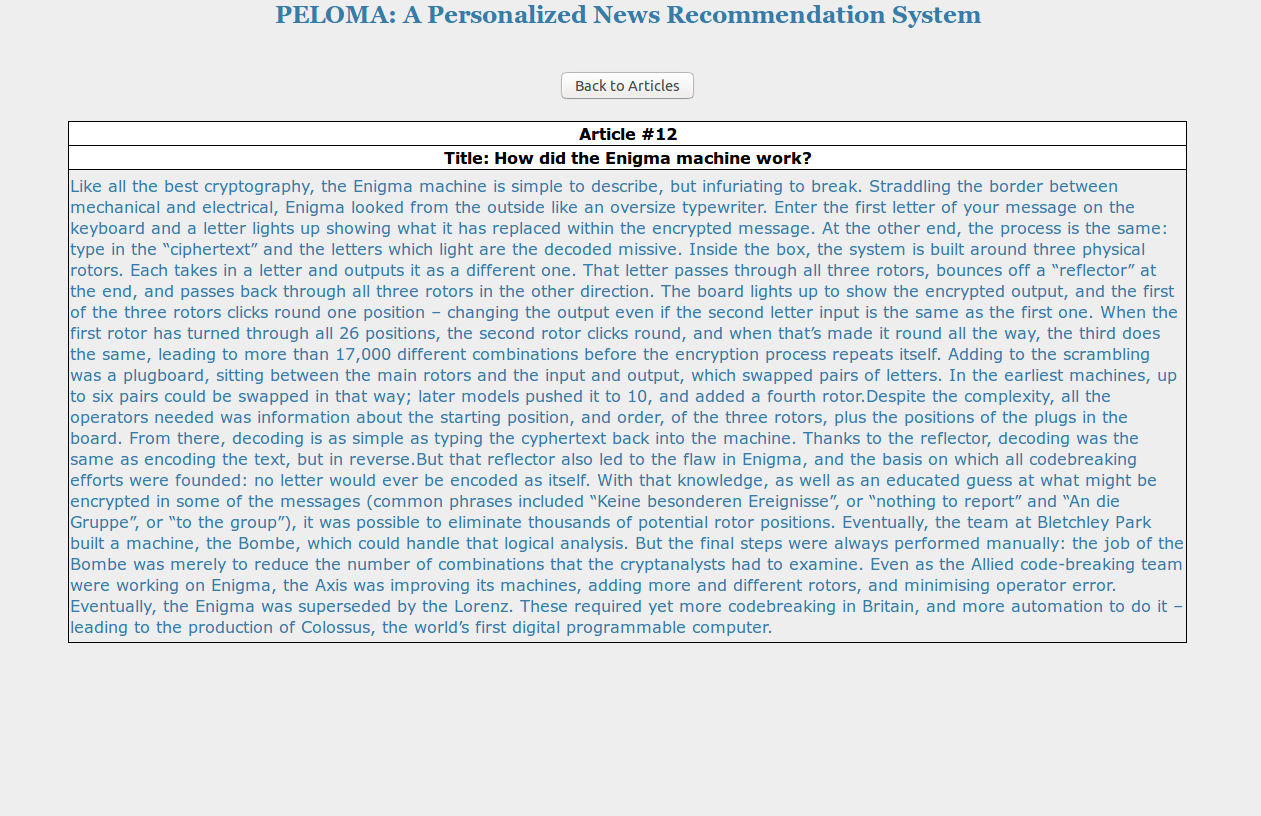
\includegraphics[scale=0.4]{static/figures/peloma/article.png}}
    \caption{Προβολή πλήρους κειμένου ενός άρθρου.}
    \label{}
\end{figure} 

\newpage

Κάθε άρθρο που αναγνώσθηκε αποθηκεύεται στη βάση δεδομένων στο ιστορικό ανάγνωσης 
του εν λόγω χρήστη. Ο χρήστης μπορεί ανά πάσα στιγμή να ενημερωθεί για τα άρθρα που έχει διαβάσει, 
μέσω του κουμπιού \textit{{\en {Reading history}}} που βρίσκεται στο επάνω μέρος της αρχικής σελίδας. \\

Αφού ο χρήστης περιηγηθεί μέσω της εφαρμογής διαβάζοντας άρθρα που τον ενδιαφέρουν, 
μπορεί να δεχθεί τις προσωποποιημένες συστάσεις άρθρων του συστήματος, 
πατώντας το κουμπί \textit{{\en {Recommendations for you}}} που βρίσκεται στο επάνω μέρος της σελίδας. 
Τότε, το σύστημα εμφανίζει μία λίστα με άρθρα που είναι πιθανό να τον ενδιαφέρουν, χωρισμένα σε κατηγορίες. 
Κάθε λίστα συστάσεων μπορεί να περιέχει άρθρα από το πολύ τρεις διαφορετικές κατηγορίες, 
δεδομένης της προτίμησης των χρηστών προς συγκεκριμένες κατηγορίες άρθρων. 
Για κάθε προτεινόμενο άρθρο αναγράφονται το {\en {id}} της κατηγορίας στην οποία ανήκει, 
το {\en {id}} και ο τίτλος του άρθρου, ο οποίος τίτλος αποτελεί και {\en {link}} προς το πλήρες κείμενο. \\
Το σύστημα εμφανίζει διαφορετικό αριθμό προτεινόμενων άρθρων ανά κατηγορία, 
ανάλογα με το ενδιαφέρον του χρήστη ως προς τη συγκεκριμένη θεματική ενότητα. \\

\begin{figure}[!ht] \centering
\centerline{
    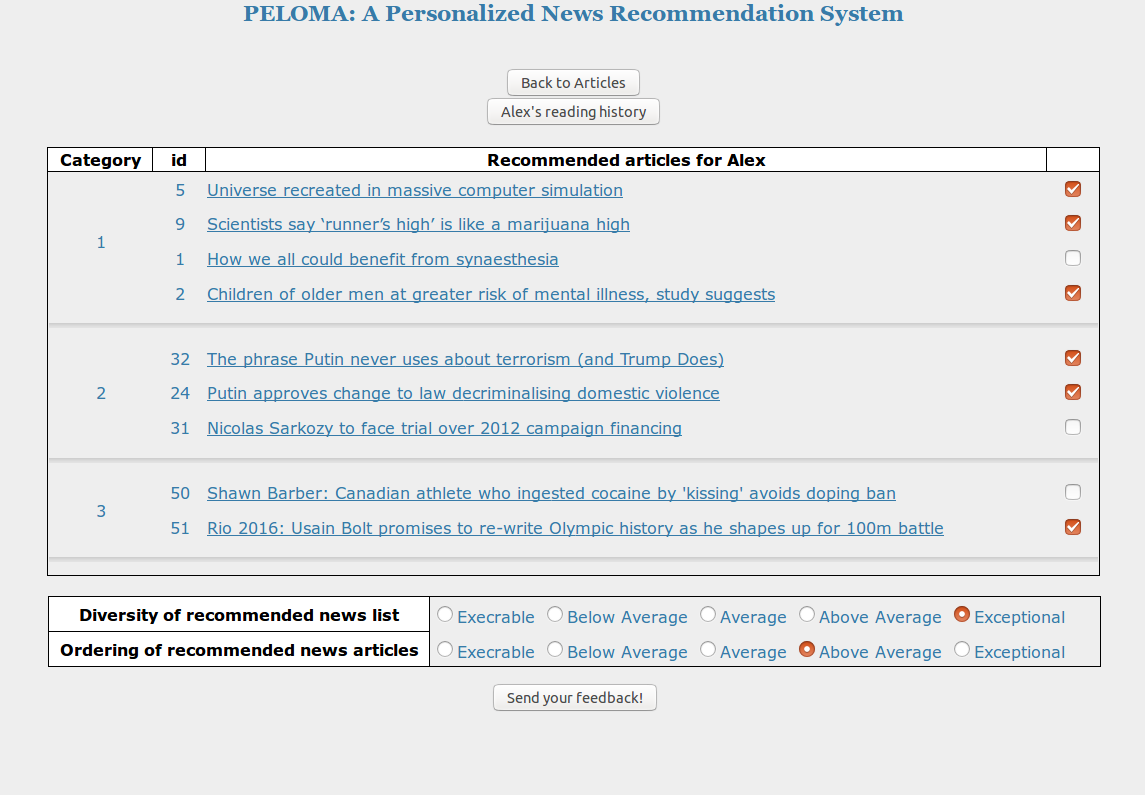
\includegraphics[scale=0.55]{static/figures/peloma/recommend.png}}
    \caption{Προβολή προσωποποιημένων συστάσεων.}
    \label{}
\end{figure} 

\newpage
Τέλος, ο χρήστης έχει την επιλογή να αξιολογήσει την ποιότητα των προσωποποιημένων συστάσεων του συστήματος. 
Μέσω των {\en {checkboxes}} που εμφανίζονται δίπλα στα άρθρα, 
μπορεί να επιλέξει τις προτάσεις του συστήματος που σχετίζονται πραγματικά με τα ενδιαφέροντά του. 
Ακριβώς κάτω από τη φόρμα συστάσεων μπορεί να αξιολογήσει το σύστημα 
τόσο ως προς την ποικιλία της λίστας συστάσεων, όσο και ως προς την κατάταξη των άρθρων της λίστας.\\

To {\en {feedback}} του χρήστη δίνεται στο σύστημα πατώντας το κουμπί {\en {Send your feedback!}}. \\
% \newpage

Ο αριθμός των άρθρων που ο χρήστης βρήκε ενδιαφέροντα αναγράφεται σε μορφή ποσοστού 
ως προς το συνολικό αριθμό προτεινόμενων άρθρων. \\

\begin{figure}[!ht] \centering
\centerline{
    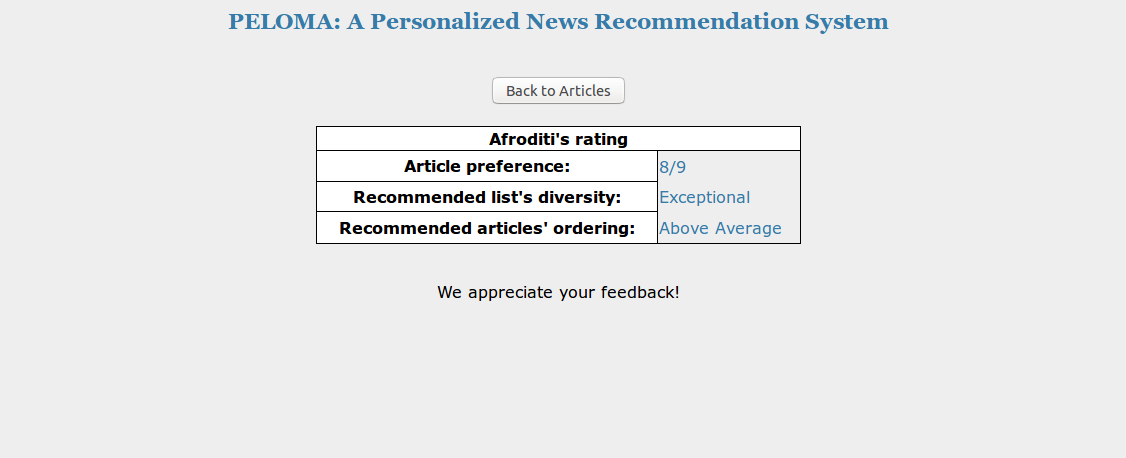
\includegraphics[scale=0.43]{static/figures/peloma/feedback2.png}}
    \caption{Αξιολόγηση συστήματος από το χρήστη.}
    \label{}
\end{figure} 

Ο χρήστης μπορεί είτε να αποσυνδεθεί από το σύστημα, είτε να συνεχίσει την ανάγνωση περισσότερων άρθρων, 
δεχόμενος εκ νέου συστάσεις. 
	\chapter{Αξιολόγηση Συστήματος}
Στο κεφάλαιο αυτό γίνεται αξιολόγηση του μηχανισμού συστάσεων του συστήματος που υλοποιήσαμε 
για τις προσωποποιημένες προτάσεις άρθρων ειδήσεων σε μεμονωμένους χρήστες. \\

Εφόσον ο στόχος του συστήματος είναι η παραγωγή χρήσιμων ως προς τους χρήστες συστάσεων, 
πραγματοποιήσαμε ένα πείραμα για να ελέγξουμε την ακρίβεια της λειτουργίας αυτής. 
Το πείραμα βασίστηκε στην αξιολόγηση του συστήματος από 50 χρήστες.
Οι εθελοντές χρήστες εισήλθαν στο σύστημα, επέλεξαν προς ανάγνωση άρθρα της αρεσκείας τους 
και το σύστημα τα καταχώρησε στο αναγνωστικό τους ιστορικό. 
Στη συνέχεια, το σύστημα δημιούργησε σύνολα προτάσεων για καθέναν από αυτούς. 
Η ικανοποίηση κάθε χρήστη υπολογίσθηκε ως προς τα εξής τρία κριτήρια: 
\begin{itemize}
  \item Συσχετισμός των προτεινόμενων άρθρων με τα πραγματικά του ενδιαφέροντα ({\en {Preference}})
  \item Ποικιλία της λίστας συστάσεων ({\en {Diversity}})
  \item Kατάταξη των άρθρων της λίστας συστάσεων ({\en {Ordering}})
\end{itemize}

\newpage

Τα αποτελέσματα του πειράματος παρουσιάζονται στο παρακάτω ιστόγραμμα: \\

\begin{figure}[!ht] \centering
\centerline{
    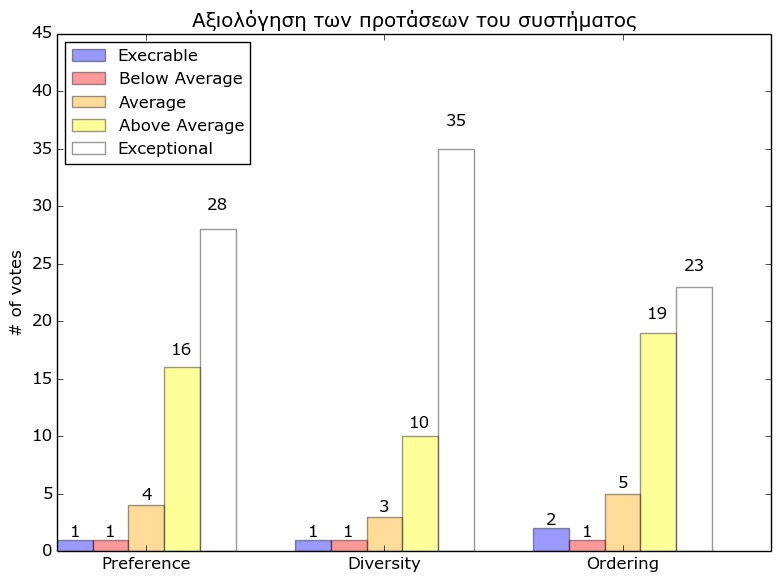
\includegraphics[scale=0.7]{static/figures/plots/plot1.png}}
    \caption{Αξιολόγηση των προτάσεων του συστήματος.}
    \label{}
\end{figure} 

Το συμπέρασμα που εξάγουμε από την πειραματική διαδικασία είναι ότι 
η πλειοψηφία των χρηστών επωφελείται από τις συστάσεις που παράγει το σύστημα, 
καθώς το μεγαλύτερο ποσοστό των χρηστών δηλώνει ικανοποιημένο ως προς τις απαιτήσεις 
για άρθρα σχετικά με τα ενδιαφέροντά του, ποικιλία στη λίστα συστάσεων 
και σωστή κατάταξη των άρθρων στην τελική λίστα. 
Συγκεκριμένα, ιδιαίτερα ικανοποιητικά είναι τα αποτελέσματα σχετικά με την ποικιλία της λίστας 
συστάσεων, όπου το σύστημα φαίνεται να εναρμονίζεται πλήρως με τα 
ενδιαφέροντα του χρήστη και να μην αφήνει καμία απ'τις ενδιαφέρουσες κατηγορίες 
άρθρων εκτός της τελικής σύστασης. \\

Άξιο καταγραφής αποτελεί και το πώς διαμορφώνονται οι συστάσεις προς έναν χρήστη 
κατά το χρόνο παραμονής του στο σύστημα, όπου δέχεται συστάσεις και συνεχίζει 
την ανάγνωση άρθρων. 
Κάθε λίστα συστάσεων περιέχει άρθρα από το πολύ τρεις διαφορετικές κατηγορίες, 
λαμβάνοντας υπόψη την τάση των χρηστών να προτιμούν συγκεκριμένες κατηγορίες άρθρων. \\

Στον Πίνακα 5.1 αποτυπώνονται οι πληροφορίες που αφορούν έναν τυχαίο χρήστη 
τη στιγμή που επιλέγει για πρώτη φορά να δεχθεί τις συστάσεις άρθρων του συστήματος. 
Στον πίνακα καταγράφονται το ιστορικό ανάγνωσης του χρήστη, 
δηλαδή ο αριθμός των άρθρων που έχουν αναγνωσθεί από κάθε κατηγορία έως τη δεδομένη στιγμή, 
η τιμή ομοιότητας του χρήστη με κάθε κατηγορία άρθρων, καθώς και ο αριθμός προτεινόμενων άρθρων 
από τις επιλεγμένες τρεις κατηγορίες με τη μεγαλύτερη ομοιότητα. \\

% ============================== 1 ===================================
\begin{table}[h]
\centering
\begin{center}
\begin{tabular}{|c|c|c|c|}
\hline
\cellcolor{blizzardblue}{\textit{\en {1st Recommendation}}}
& \multicolumn{1}{|p{3cm}|}{\centering \textbf{{\en {\# of articles }} \\ {\en {in user's}} \\ {\en {history}}}} 
& \multicolumn{1}{|p{3cm}|}{\centering \textbf{{\en {Similarity }} \\ {\en {with}} \\ {\en {Category}}}} 
& \multicolumn{1}{|p{3cm}|}{\centering \textbf{{\en {\# of }} \\ {\en {recommended articles}}}}\\
\hline
\multicolumn{1}{|p{3.8cm}|}{\centering \textbf{{\en {Category \#}1}}} & 4 & 0.2607 & 0 \\
\hline
\rowcolor{classicrose}
\multicolumn{1}{|p{3.8cm}|}{\centering \textbf{{\en {Category \#}2}}} & \textbf{6} & \textbf{0.3544} & \textbf{3} \\
\hline
\rowcolor{classicrose}
\multicolumn{1}{|p{3.8cm}|}{\centering \textbf{{\en {Category \#}3}}} & \textbf{7} & \textbf{0.3638} & \textbf{4} \\
\hline
\multicolumn{1}{|p{3.8cm}|}{\centering \textbf{{\en {Category \#}4}}} & 4 &  0.2469 & 0 \\
\hline
\multicolumn{1}{|p{3.8cm}|}{\centering \textbf{{\en {Category \#}5}}} & 4 & 0.3427 & 0 \\
\hline
\rowcolor{classicrose}
\multicolumn{1}{|p{3.8cm}|}{\centering \textbf{{\en {Category \#}6}}} & \textbf{4} & \textbf{0.3466} & \textbf{2} \\
\hline
\multicolumn{1}{|p{3.8cm}|}{\centering \textbf{{\en {Category \#}7}}} & 2 & 0.26788 & 0 \\
\hline
\end{tabular}
\caption{Ιστορικό ανάγνωσης και 1η φάση συστάσεων}
\end{center}
\label{table05.01}
\end{table}

% ====================================================================

Παρατηρούμε πως το σύστημα εντόπισε ορθώς την προτίμηση του χρήστη για τις τρεις αυτές κατηγορίες, 
δεδομένου ότι είναι και αυτές από τις οποίες έχει αναγνώσει το μεγαλύτερο αριθμό άρθρων. 
Λαμβάνοντας υπόψη το μικρό αριθμό άρθρων που έχουμε αποθηκευμένα στη βάση δεδομένων από κάθε κατηγορία, 
ο αλγόριθμος του συστήματος έχει σχεδιαστεί να προτείνει τέσσερα άρθρα από την πιο ταιριαστή κατηγορία, 
τρία άρθρα από τη δεύτερη πιο ταιριαστή και δύο άρθρα από την τρίτη σε σειρά πιο ταιριαστή κατηγορία. 
Αυτή η παραδοχή προϋποθέτει την ύπαρξη του αντίστοιχου αριθμού άρθρων μέσα στην επιλεγμένη ομάδα {\en {(group)}}
κάθε επιλεγμένης κατηγορίας {\en {(cluster)}}. \\

\begin{figure}[!ht] \centering
\centerline{
    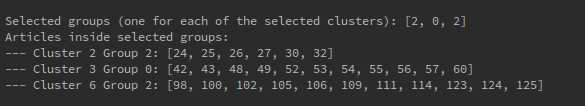
\includegraphics[scale=0.7]{static/figures/peloma/select3.png}}
    \caption{Επιλεγμένες ομάδες από κάθε κατηγορία.}
    \label{fig:select1}
\end{figure} 

Στην Εικόνα \ref{fig:select1} αποτυπώνονται οι ομάδες άρθρων που επιλέχθηκαν και οι οποίες μας οδήγησαν 
στην 1η φάση συστάσεων άρθρων. Μερικά από τα άρθρα εντός των επιλεγμένων ομάδων έχουν ήδη 
αναγνωσθεί από το χρήστη και είναι αυτά που οδήγησαν το σύστημα να συμπεράνει την ομοιότητα. 
Έτσι, γίνεται εύκολα αντιληπτό ότι εξαιτίας του περιορισμένου αριθμού άρθρων στη βάση δεδομένων, 
είναι πιθανό η ομοιότητα ενός χρήστη με μία κατηγορία να αυξάνεται καθώς αυτός συνεχίζει να 
επιλέγει άρθρα από την εν λόγω κατηγορία, όμως να μην υπάρχει διαθέσιμος ο επιθυμητός αριθμός 
άρθρων προς σύσταση. \\

Στον Πίνακα 5.2 αποτυπώνονται το ιστορικό ανάγνωσης του χρήστη, 
η τιμή ομοιότητας του χρήστη με κάθε κατηγορία άρθρων και η δεύτερη φάση συστάσεων. 
Παρατηρούμε πως ο χρήστης επέλεξε να αναγνώσει τόσο άρθρα από τις προτεινόμενες κατηγορίες, 
όσο και ένα άρθρο από την Κατηγορία {\en {\#5}}, εξ ου και η αύξηση της ομοιότητάς του με την κατηγορία αυτή. 
Το σύστημα εξακολουθεί να συμπεριφέρεται ορθά, δίνοντας μεγαλύτερη βαρύτητα στην Κατηγορία {\en {\#6}}. \\

% ============================ 2 ===================================

\begin{table}[h]
\centering
\begin{center}
\begin{tabular}{|c|c|c|c|}
\hline
\cellcolor{blizzardblue}{\textit{\en {2nd Recommendation}}}
& \multicolumn{1}{|p{3cm}|}{\centering \textbf{{\en {\# of articles }} \\ {\en {in user's}} \\ {\en {history}}}} 
& \multicolumn{1}{|p{3cm}|}{\centering \textbf{{\en {Similarity }} \\ {\en {with}} \\ {\en {Category}}}} 
& \multicolumn{1}{|p{3cm}|}{\centering \textbf{{\en {\# of }} \\ {\en {recommended articles}}}}\\
\hline
\multicolumn{1}{|p{3.9cm}|}{\centering \textbf{{\en {Category \#}1}}} & 4 & 0.2846 & 0 \\
\hline
\multicolumn{1}{|p{3.9cm}|}{\centering \textbf{{\en {Category \#}2}}} & 9 & 0.3273 & 0 \\
\hline
\rowcolor{classicrose}
\multicolumn{1}{|p{3.9cm}|}{\centering \textbf{{\en {Category \#}3}}} & \textbf{7} & \textbf{0.3566} & \textbf{2} \\
\hline
\multicolumn{1}{|p{3.9cm}|}{\centering \textbf{{\en {Category \#}4}}} & 4 &  0.2513 & 0 \\
\hline
\rowcolor{classicrose}
\multicolumn{1}{|p{3.9cm}|}{\centering \textbf{{\en {Category \#}5}}} & \textbf{5} & \textbf{0.3677} & \textbf{3} \\
\hline
\rowcolor{classicrose}
\multicolumn{1}{|p{3.9cm}|}{\centering \textbf{{\en {Category \#}6}}} & \textbf{5} & \textbf{0.3919} & \textbf{4} \\
\hline
\multicolumn{1}{|p{3.9cm}|}{\centering \textbf{{\en {Category \#}7}}} & 2 & 0.2696 & 0 \\
\hline
\end{tabular}
\caption{Ιστορικό ανάγνωσης και 2η φάση συστάσεων}
\end{center}
\label{table05.02}
\end{table}
% ====================================================================

\begin{comment}
Επιπρόσθετα, αξίζει να αναφέρουμε πως παρόλο που ο χρήστης επέλεξε να διαβάσει τα τρία προτεινόμενα 
άρθρα της Κατηγορίας {\en {\#2}}, φτάνοντας συνολικά στα εννιά διαβασμένα άρθρα από την κατηγορία αυτή, 
η ομοιότητά του με την εν λόγω κατηγορία υπολογίσθηκε τελικά μικρότερη σε σχέση με πριν. 
Επιλέγουμε να χρησιμοποιήσουμε το συγκεκριμένο σενάριο χρήσης του συστήματος και όχι κάποιο πιο ιδανικό, 
καθώς στην περίπτωση αυτή αναδεικνύεται ένα πρόβλημα των πιθανοτικών μοντέλων θεμάτων, όπου για κάθε άρθρο 
επιλέγουμε έναν αντιπροσωπευτικό αριθμό λέξεων και όχι ολόκληρο το κείμενό του.
Με τον ίδιο τρόπο επιδρούσαν τα μοντέλα θεμάτων πάνω στα {\en {clusters}} και τα {\en {groups}}, 
εξάγοντας έναν σαφώς μεγαλύτερο αριθμό αντιπροσωπευτικών λέξεων, που πιθανόν ``αδικεί'' 
ως προς το τελικό λεξιλόγιο κάποια από τα άρθρα που περιέχονται στα εν λόγω {\en {clusters}} και {\en {groups}}. 
Έτσι, αν οι λέξεις που χαρακτηρίζουν τα προσφάτως διαβασμένα άρθρα της Κατηγορίας {\en {\#2}} 
δεν αποτελούν μεγάλο μέρος του λεξιλογίου της κατηγορίας, είναι λογικό η ομοιότητα με την κατηγορία 
να μην αυξηθεί αισθητά και να μην έχουμε εκ νέου σχετικές συστάσεις. \\
\end{comment}

Στον Πίνακα 5.3 αποτυπώνονται το ιστορικό ανάγνωσης του χρήστη, 
η τιμή ομοιότητας του χρήστη με κάθε κατηγορία άρθρων και η τρίτη φάση συστάσεων. 
Παρατηρούμε πως το σύστημα λειτουργεί ομαλά, επιστρέφοντας ξανά συστάσεις 
από την Κατηγορία {\en {\#2}}, απ' όπου ο χρήστης έχει διαβάσει και το μεγαλύτερο 
αριθμό άρθρων. \\

\newpage 

% =============================== 3 =================================

\begin{table}[h]
\centering
\begin{center}
\begin{tabular}{|c|c|c|c|}
\hline
\cellcolor{blizzardblue}{\textit{\en {3rd Recommendation}}}
& \multicolumn{1}{|p{3cm}|}{\centering \textbf{{\en {\# of articles }} \\ {\en {in user's}} \\ {\en {history}}}} 
& \multicolumn{1}{|p{3cm}|}{\centering \textbf{{\en {Similarity }} \\ {\en {with}} \\ {\en {Category}}}} 
& \multicolumn{1}{|p{3cm}|}{\centering \textbf{{\en {\# of }} \\ {\en {recommended articles}}}}\\
\hline
\multicolumn{1}{|p{3.8cm}|}{\centering \textbf{{\en {Category \#}1}}} & 4 & 0.2853 & 0 \\
\hline
\rowcolor{classicrose}
\multicolumn{1}{|p{3.8cm}|}{\centering \textbf{{\en {Category \#}2}}} & \textbf{12} & \textbf{0.3837} & \textbf{2} \\
\hline
\multicolumn{1}{|p{3.8cm}|}{\centering \textbf{{\en {Category \#}3}}} & 8 & 0.3578 & 0 \\
\hline
\multicolumn{1}{|p{3.8cm}|}{\centering \textbf{{\en {Category \#}4}}} & 4 &  0.2779 & 0 \\
\hline
\rowcolor{classicrose}
\multicolumn{1}{|p{3.8cm}|}{\centering \textbf{{\en {Category \#}5}}} & \textbf{6} & \textbf{0.4013} & \textbf{3} \\
\hline
\rowcolor{classicrose}
\multicolumn{1}{|p{3.8cm}|}{\centering \textbf{{\en {Category \#}6}}} & \textbf{7} & \textbf{0.4026} & \textbf{4} \\
\hline
\multicolumn{1}{|p{3.8cm}|}{\centering \textbf{{\en {Category \#}7}}} & 2 & 0.3012 & 0 \\
\hline
\end{tabular}
\caption{Ιστορικό ανάγνωσης και 3η φάση συστάσεων}
\end{center}
\label{table05.03}
\end{table}
% ====================================================================

Το σύστημα καλύπτει επαρκώς τις αναγνωστικές ανάγκες του χρήστη, 
καθώς κατά τις τρεις διαφορετικές φάσεις έγιναν συστάσεις από τέσσερις διαφορετικές κατηγορίες άρθρων, 
από τις οποίες είχε διαβαστεί ένας σημαντικός αριθμός άρθρων. \\

% =======================================================================
Τέλος, ως μέρος της πειραματικής ανάλυσης επιλέγουμε να παραθέσουμε και ένα σενάριο χρήσης του συστήματος 
όπου ένας χρήστης με κενό αναγνωστικό ιστορικό 
συνδέεται στο σύστημα και επιλέγει προς ανάγνωση άρθρα μόνο από μία κατηγορία, 
την Κατηγορία {\en {\#}}1. 
Πρώτη επιλογή προς ανάγνωση αποτελεί το άρθρο {\en {\#}}12. \\
Σκοπός μας είναι να διαπιστώσουμε αν το σύστημα θα λειτουργήσει ορθώς, 
προτείνοντας στο χρήστη άρθρα μόνο από τη συγκεκριμένη κατηγορία, καθώς και να 
παρατηρήσουμε τον τρόπο με τον οποίο επιλέγονται τα άρθρα από το πιο όμοιο γκρουπ 
έως το λιγότερο όμοιο, καθώς ο χρήστης συνεχίζει την ανάγνωση  των προτεινόμενων άρθρων 
μέχρι την εξάντληση όλων των διαθέσιμων άρθρων της κατηγορίας αυτής. \\

\begin{figure}[!ht] \centering
\centerline{
    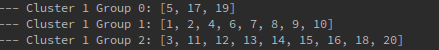
\includegraphics[scale=0.85]{static/figures/category/1.png}}
    \caption{{\en {Groups}} άρθρων της Κατηγορίας {\en {\#}}1.}
    \label{}
\end{figure} 

\begin{figure}[!ht] \centering
\centerline{
    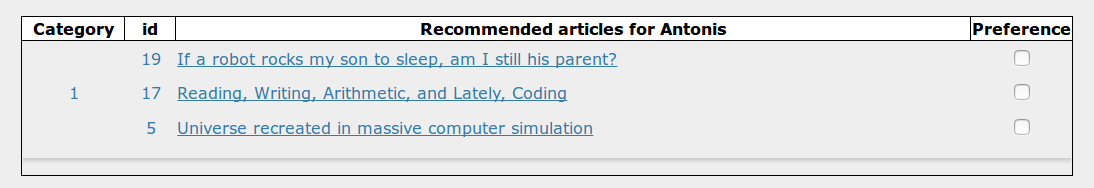
\includegraphics[scale=0.43]{static/figures/category/1a.png}}
    \caption{Κατηγορία {\en {\#}}1 - 1η σύσταση - Άρθρα από {\en {group 0}} .}
    \label{}
\end{figure} 

\begin{figure}[!ht] \centering
\centerline{
    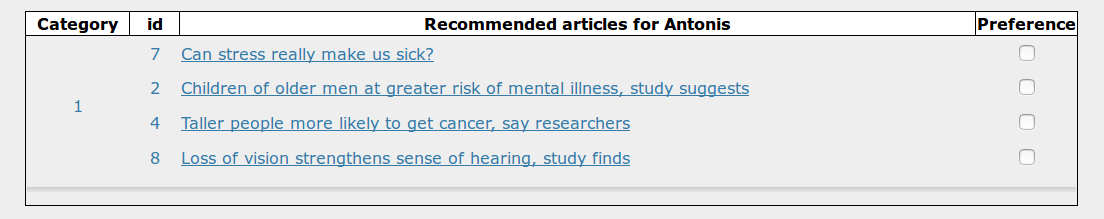
\includegraphics[scale=0.43]{static/figures/category/1b.png}}
    \caption{Κατηγορία {\en {\#}}1 - 2η σύσταση - Άρθρα από {\en {group 1}} .}
    \label{}
\end{figure} 

\begin{figure}[!ht] \centering
\centerline{
    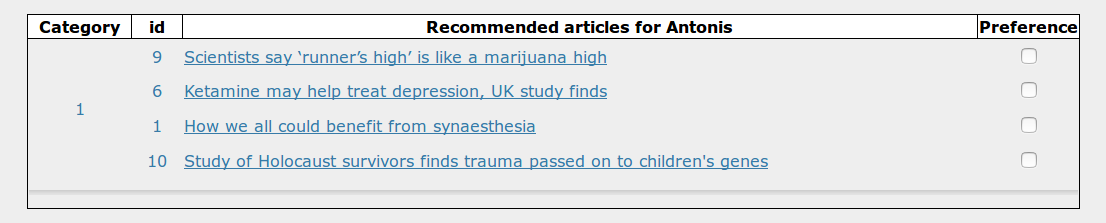
\includegraphics[scale=0.43]{static/figures/category/1c.png}}
    \caption{Κατηγορία {\en {\#}}1 - 3η σύσταση - Άρθρα από {\en {group 1}} .}
    \label{}
\end{figure} 
\begin{figure}[!ht] \centering
\centerline{
    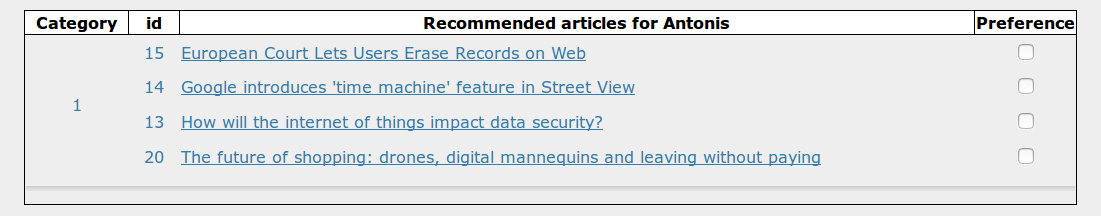
\includegraphics[scale=0.43]{static/figures/category/1d.png}}
    \caption{Κατηγορία {\en {\#}}1 - 4η σύσταση - Άρθρα από {\en {group 2}} .}
    \label{}
\end{figure} 

\begin{figure}[!ht] \centering
\centerline{
    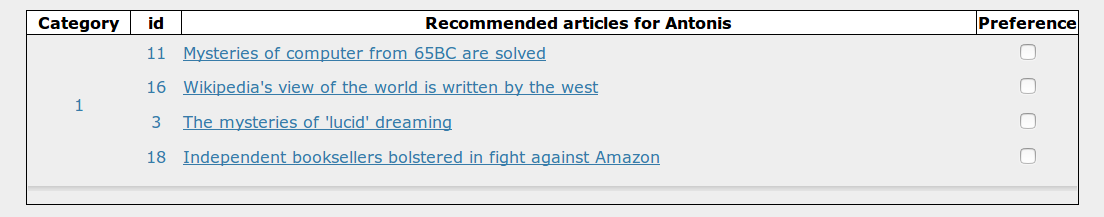
\includegraphics[scale=0.43]{static/figures/category/1e.png}}
    \caption{Κατηγορία {\en {\#}}1 - 5η σύσταση - Άρθρα από {\en {group 2}} .}
    \label{}
\end{figure} 

\newpage 

Κλείνοντας, η πειραματική αξιολόγηση έδειξε πως το σύστημα είναι σε θέση 
να καλύψει επαρκώς τις αναγνωστικές ανάγκες του χρήστη με βάση τα δεδομένα 
που του έχουν δοθεί ως είσοδος. 
Επιπλέον, μπορούμε να παρατηρήσουμε ότι σε ένα τέτοιο σύστημα 
είναι δύσκολο να πραγματοποιηθεί μια αντικειμενική αξιολόγηση, 
καθώς οι προτιμήσεις του χρήστη διαφέρουν από αυτές των υπολοίπων χρηστών 
ή ακόμα και από τις δικές του, ανάλογα με τις περιστάσεις. 

	\chapter{\selectlanguage{greek}Συμπεράσματα και Μελλοντικές Επεκτάσεις}

\section{\selectlanguage{greek}Συμπεράσματα}

Καθώς όλο και περισσότερες πληροφορίες γίνονται διαθέσιμες στο διαδίκτυο, οι
χρήστες όλο και περισσότερο ψάχνουν απεγνωσμένα κάποια εργαλεία που θα τους
βοηθήσουν να φιλτράρουν αυτή τη ροή των πληροφοριών και να βρουν άρθρα
ειδήσεων που να τους ενδιαφέρουν. Ακριβώς σε ένα τέτοιο σενάριο, το σύστημα που
αναπτύχθηκε στο πλαίσιο αυτής της διπλωματικής εργασίας προσπαθεί να περιορίσει το πρόβλημα που
δημιουργείται από την διαρκή ροή ειδήσεων από διαφορετικές πηγές ενημέρωσης.
Αυτό που ουσιαστικά θέλουμε να δημιουργήσουμε είναι να παρέχουμε μια
εξατομικευμένη υπηρεσία συστάσεων για άρθρα ειδήσεων, στην οποία ο χρήστης 
θα επιλέγει τις κατηγορίες σχετικά με τις οποίες θέλει να ενημερώνεται και με βάση 
το προφίλ του και το ιστορικό χρήσης, το σύστημα θα παρέχει εξατομικευμένες συστάσεις 
που ταιριάζουν περισσότερο με τα ενδιαφέροντά του. \\

Στο πλαίσιο της εργασίας παρουσιάσαμε ένα σύστημα δημιουργίας εξατομικευμένων συστάσεων 
σε εφαρμογή διαδικτυακού περιεχομένου, 
η οποία λαμβάνει υπόψη το προφίλ και το ιστορικό των χρηστών του συστήματος για να 
προτείνει άρθρα ειδήσεων. 
Τα άρθρα αναπαρίστανται με τη βοήθεια θεματικών μοντέλων, 
δηλαδή μοντέλων για την ανακάλυψη θεμάτων που υπάρχουν σε μία συλλογή κειμένων. 
Τα προφίλ των χρηστών αναπαρίστανται μέσω μιας τριπλέτας αποτελούμενης από 
τα εξής χαρακτηριστικά: την κατανομή των θεμάτων των αναγνωσμένων άρθρων, 
τη λίστα χρηστών οι οποίοι έχουν παρόμοια πρότυπα πρόσβασης με τον εν λόγω χρήστη και 
τέλος, τη λίστα από ονοματισμένες οντότητες, δηλαδή λέξεις οι οποίες απαντούν σε φράσεις όπως 
``Τι συνέβη, ποιος εμπλέκεται, πότε συνέβη'' κλπ. 
Στόχος μας ήταν να βρούμε σύντομες περιγραφές των άρθρων της συλλογής και 
να εξερευνήσουμε τους συσχετισμούς μεταξύ των {\en {clusters}} (ή
των {\en {groups}}) άρθρων και του προφίλ του δοθέντος χρήστη, 
συγκρίνοντας την ομοιότητα των θεμάτων που “κρύβονται” μέσα στα άρθρα τους.
Οι σχέσεις μεταξύ αυτών των εννοιών εμπλουτίζουν τις παραπάνω αναπαραστάσεις 
και ενσωματώνονται στις διαδικασίες δημιουργίας συστάσεων. \\

Πιο συγκεκριμένα, συλλέξαμε άρθρα ειδήσεων τόσο από τον παγκόσμιο ιστό, όσο και από τη συλλογή {\en {Reuters}} του {\en {NLTK}} 
και τα αποθηκεύσαμε σε μία βάση δεδομένων. 
Το λειτουργικό μέρος του μηχανισμού εξάγει χρήσιμο κείμενο από αυτά, πραγματοποιεί μεθόδους εξαγωγής λέξεων
κλειδιών από κάθε άρθρο που υπάρχει στο σύστημα, εφαρμόζει τα θεματικά μοντέλα σε κάθε κατηγορία, γκρουπ και άρθρο, 
επιτρέποντας με αυτό τον τρόπο την περαιτέρω επεξεργασία τους βάσει σημασιολογικών συσχετίσεων μεταξύ των άρθρων.
Το ορατό στους χρήστες είναι ο δικτυακός τόπος που εμφανίζει τα άρθρα του συστήματος σημασιολογικά κατηγοριοποιημένα. 
Ο μηχανισμός προτάσεων του συστήματος, με βάση το προφίλ του χρήστη, 
παράγει ένα σύνολο εξατομικευμένων προτάσεων ειδήσεων που ταιριάζουν περισσότερο με τα
σημασιολογικά ενδιαφέροντα του χρήστη, κάνοντας δυνατή με αυτό τον τρόπο την
παρουσίαση ειδήσεων που σχετίζονται σημασιολογικά με αυτές που ήδη έχει
αναγνώσει. \\

Κατά την πειραματική αξιολόγηση του συστήματος, η ικανοποίηση κάθε χρήστη υπολογίσθηκε ως προς τα εξής τρία κριτήρια: 
συσχετισμός των προτεινόμενων άρθρων με τα πραγματικά του ενδιαφέροντα ({\en {Preference}}), 
ποικιλία της λίστας συστάσεων ({\en {Diversity}}) και 
κατάταξη των άρθρων της λίστας συστάσεων ({\en {Ordering}}). 
Επιπρόσθετα, παρουσιάστηκαν σενάρια χρήσης του συστήματος κατά τα οποία ο χρήστης 
είτε έχει αναγνώσει άρθρα από διάφορες κατηγορίες, είτε μόνο από μία κατηγορία 
και επιλέγει να δεχτεί τις συστάσεις του συστήματος. 
Διαπιστώθηκε ότι το σύστημα είναι σε θέση να καλύψει επαρκώς τις αναγνωστικές ανάγκες του χρήστη 
με βάση τα δεδομένα που του έχουν δοθεί ως είσοδος. 
Iδιαίτερα ικανοποιητικά είναι τα αποτελέσματα σχετικά με την ποικιλία της λίστας 
συστάσεων, όπου το σύστημα φαίνεται να εναρμονίζεται πλήρως με τα 
ενδιαφέροντα του χρήστη και να μην αφήνει καμία απ'τις ενδιαφέρουσες κατηγορίες 
άρθρων εκτός της τελικής σύστασης.\\

Από τα πειραματικά ευρήματα συμπεραίνουμε, επίσης, ότι το σύστημά μας έχει 
καλή απόδοση σε διαφορετικούς τύπους κειμένων και ιδιαίτερα, όταν τα
κείμενα είναι μικρά σε μέγεθος. Aυτό ερμηνεύεται μέσω του διανύσματος αναπαράστασης ενός κειμένου 
που προκύπτει από την εφαρμογή του αλγορίθμου {\en {LDA}}, 
στο οποίο επιλέγουμε τον αριθμό αντιπροσωπευτικών λέξεων απ'τις οποίες θα αποτελείται.
Έτσι, ένα τέτοιο διάνυσμα έχει μεγαλύτερες πιθανότητες να αποτυπώσει ορθότερα το νόημα ενός άρθρου, 
όταν το άρθρο αποτελείται από σχετικά μικρό αριθμό λέξεων. \\

Αξίζει να σημειώσουμε ότι τα θεματικά μοντέλα είναι ένα χρήσιμο εργαλείο εξερεύνησης. 
Τα θέματα παρέχουν μία περίληψη ενός σώματος κειμένων που είναι αδύνατο να γίνει με το χέρι. Η θεματική
ανάλυση μπορεί να ανακαλύψει συνδέσεις ανάμεσα και μέσα στα κείμενα που δεν είναι
φανερές με γυμνό μάτι και να βρει συσχετίσεις όρων που δε θεωρούνται δεδομένες. \\

% Ωστόσο, υπάρχουν περιθώρια βελτίωσης της απόδοσης του συστήματος,. \\
Πρόκληση για το σύστημά μας αποτελεί η αύξηση του πλήθους των άρθρων ανά κατηγορία στη βάση δεδομένων του συστήματος, 
καθώς και η αξιολόγηση των ομάδων που θα δημιουργηθούν από την εφαρμογή του αλγορίθμου {\en {k-means}} εντός κάθε κατηγορίας. \\

Τέλος, άξιο αναφοράς αποτελεί το πόσο βοηθητική υπήρξε η χρήση της 
γλώσσας προγραμματισμού {\en {Python}} σε μία τέτοια εφαρμογή 
και συγκεκριμένα η πλατφόρμα {\en {NLTK (Natural Language Toolkit)}}, 
μια πλατφόρμα με έτοιμα εργαλεία επεξεργασίας φυσικής γλώσσας. 

\section{\selectlanguage{greek}Μελλοντικές Επεκτάσεις}

Το σύστημα που αναπτύχθηκε στο πλαίσιο αυτής της διπλωματικής
εργασίας θα μπορούσε να βελτιωθεί και να επεκταθεί περαιτέρω,
τουλάχιστον ως προς τις κάτωθι κατευθύνσεις: \\

{\textbf {Συστάσεις σε ομάδες χρηστών}}\\
Η περιγραφή των προτιμήσεων με τη βοήθεια διανυσμάτων επιτρέπει το συνδυασμό
πολλαπλών προφίλ για τη δημιουργία ενός κοινού προφίλ για μια ομάδα χρηστών. \\

{\textbf {Ανατροφοδότηση του συστήματος με την αξιολόγηση του χρήστη}} \\
Το σύστημα μπορεί να δέχεται ως είσοδο την αξιολόγηση του χρήστη, 
αποθηκεύοντας στη βάση δεδομένων τα προτεινόμενα άρθρα που ο χρήστης βρήκε 
πραγματικά ενδιαφέροντα σε σχέση με ολόκληρη τη λίστα συστάσεων. 
Έτσι, μπορούν να πραγματοποιηθούν κάποιες πιο ισχυρές συνάψεις μεταξύ 
συγκεκριμένων άρθρων μέσα σε κάθε {\en {cluster}} και θεμάτων που 
διαφαίνονται από τις επιλογές ενός χρήστη, προκειμένου να λάβουμε βελτιωμένα αποτελέσματα 
σε επόμενη σύσταση. \\

{\textbf {Εφαρμογή συνάρτησης αξιολόγησης}} για την επιλογή ν-άδων σύστασης που 
προσφέρουν τη μέγιστη αύξηση ωφέλειας για το χρήστη (Εφαρμογή 
{\en {submodular}} μοντέλου συστάσεων με χρήση άπληστου προσεγγιστικού αλγορίθμου).

\begin{comment}
{\textbf {Πολυεπίπεδες υβριδικές συστάσεις}}
Το προφίλ ομάδων χρηστών χωρίζονται σε σημασιολογικούς τομείς. Καθένας από τους
τομείς αντιστοιχεί σε μια ομάδα και αντιπροσωπεύει ένα υποσύνολο των προτιμήσεων
του χρήστη που μοιράζεται με τους χρήστες που συμμετείχαν στη διαδικασία
δημιουργίας των ομάδων. Με την εισαγωγή επιπλέον δομής στα προφίλ των χρηστών
είναι δυνατό να οριστούν σχέσεις μεταξύ των χρηστών σε διαφορετικά επίπεδα,
δημιουργώντας με αυτό τον τρόπο πολύ-επίπεδες κοινότητες ενδιαφερόντων.
\end{comment}
%	\chapter{Παράδειγμα Πίνακα}

\section{Συμπεράσματα}
Τα συστήματα ομότιμων κόμβων, προκειμένου να υποστηρίζουν πιο
εκφραστικές λειτουργίες αναπαράστασης και αναζήτησης δεδομένων,
εξελίχθηκαν στα συστήματα ομότιμων κόμβων τα οποία βασίζονται στις
τεχνολογίες του Σημασιολογικού Ιστού για την αναπαράσταση των
δεδομένων μέσω σχημάτων που τα περιγράφουν (\en{Schema-based
peer-to-peer systems}).

Συμπερασματικά το σύστημα που αναπτύχθηκε στα πλαίσια αυτής της
διπλωματικής είναι ένα πλήρες σύστημα ομότιμων κόμβων βασισμένο σε
σχήματα, το οποίο καθιστά δυνατή την αναζήτηση της πληροφορίας με
ένα διαφορετικό τρόπο απ' ότι τα προϋπάρχοντα  συστήματα.

\section{Μελλοντικές Επεκτάσεις}
Το σύστημα που αναπτύχθηκε στα πλαίσια αυτής της διπλωματικής
εργασίας θα μπορούσε να βελτιωθεί και να επεκταθεί περαιτέρω,
τουλάχιστον ως προς τρεις κατευθύνσεις. Συγκεκριμένα, αναφέρονται
τα ακόλουθα:

\begin{itemize}
\item Ενσωμάτωση διαδικασίας επιλογής σχήματος με βάση το οποίο ο
κόμβος θα συμμετέχει στο σύστημα. Έτσι όπως έχει σχεδιαστεί το
σύστημα, κάθε κόμβος έχει τη δυνατότητα να δημιουργήσει πολλά
σχήματα και να αποθηκεύσει δεδομένα σε περισσότερα από ένα. Ως
σχήμα του κόμβου (με βάση το οποίο απαντάει τις ερωτήσεις),
θεωρείται το τελευταίο στο οποίο αποθήκευσε δεδομένα. Η δυνατότητα
επιλογής θα του παρείχε περισσότερη ευελιξία.
\item Δυνατότητα αντιστοίχισης δεδομένων τα οποία να μην είναι
αποθηκευμένα σε βάση δεδομένων αλλά σε αρχεία. Η αποδέσμευση από
τη βάση δεδομένων θα έκανε το σύστημα πιο εύκολο στην εγκατάσταση
και τη χρήση.
\item Αξιολόγηση του συστήματος ως προς τη συμπεριφορά του αν
συμμετέχει σε αυτό μεγάλος αριθμός κόμβων \en{(scalability
testing)} και αν χρησιμοποιηθεί ένα πολύ μεγάλο καθολικό σχήμα. H
αξιολόγηση αυτή αφορά την ταχύτητα με την οποία ένας κόμβος
παίρνει απαντήσεις σε μια ερώτηση καθώς και την ποιότητα των
απαντήσεων.
\end{itemize}

%
	\begin{table}[!tb]
		\centering
		\caption{Πίνακας αλήθειας της λογικής συνάρτησης \en{F}}
		\small
		\renewcommand{\arraystretch}{1.3}
		\begin{tabular}{| c | c | c || c |}
			\hline               
		  	\textbf{\en{A}} & \textbf{\en{B}} &  \textbf{\en{C}} &   \textbf{\en{F}} \\
			\hline
				  0 & 0 & 0 & 0  \\
				  0 & 0 & 1 & 0  \\
				  0 & 1 & 0 & 1  \\
				  0 & 1 & 1 & 0  \\	
				  1 & 0 & 0 & 1  \\
				  1 & 0 & 1 & 0  \\
				  1 & 1 & 0 & 1  \\
				  1 & 1 & 1 & 0  \\
		  	\hline
		\end{tabular}
		\label{table07.01}
	\end{table}
%
%	\chapter{Παράδειγμα Μαθηματικών Σχέσεων -- Εκφράσεων}

\section{Συμπεράσματα}
Τα συστήματα ομότιμων κόμβων, προκειμένου να υποστηρίζουν πιο
εκφραστικές λειτουργίες αναπαράστασης και αναζήτησης δεδομένων,
εξελίχθηκαν στα συστήματα ομότιμων κόμβων τα οποία βασίζονται στις
τεχνολογίες του Σημασιολογικού Ιστού για την αναπαράσταση των
δεδομένων μέσω σχημάτων που τα περιγράφουν (\en{Schema-based
peer-to-peer systems}).

Στα συστήματα αυτά κάθε \en{$\displaystyle y=\int_0^1f(x)dx$} \en{$y=\int_0^1f(x)dx$} κόμβος χρησιμοποιεί ένα σχήμα για την \en{$\displaystyle \sum_{i=0}^{100}a_i$}
αναπαράσταση των δεδομένων του. Όμως σε ένα σύστημα ομότιμων
κόμβων, κάθε κόμβος έχει διαφορετικές απαιτήσεις αναπαράστασης
δεδομένων. Επομένως πρέπει να υπάρχει ευελιξία στην επιλογή \en{$\displaystyle \frac{1}{1+x^2}$}
σχήματος. Τα συστήματα που έχουν προταθεί μέχρι τώρα και παρέχουν
αυτή την ευελιξία, για να είναι δυνατή η αναζήτηση πληροφορίας,
απαιτούν την ύπαρξη κανόνων αντιστοίχισης μεταξύ των σχημάτων με
βάση τους οποίους να μετασχηματίζονται οι ερωτήσεις. Όμως δεν
υποστηρίζεται ακόμα αυτόματη δημιουργία και δυναμική ανανέωση των
κανόνων, που είναι απαραίτητα για τα συστήματα ομότιμων κόμβων.
\begin{equation}
	y=\int_0^1f(x)dx
	\label{equation08.01}
\end{equation}

Η συνεισφορά της (\ref{equation08.01}) παρούσας διπλωματικής εργασίας έχει δύο σκέλη. Το
πρώτο αφορά τη δημιουργία ενός πλήρους συστήματος ομότιμων κόμβων
βασισμένο σε σχήματα \en{RDF} το οποίο παρέχει: (α) την υποδομή
για την επικοινωνία των κόμβων,(β) μηχανισμό δημιουργίας σχήματος,
(γ) μηχανισμό ενσωμάτωσης σχεσιακών δεδομένων στο σχήμα με τη
χρήση αντιστοιχίσεων που δημιουργεί ο χρήστης με τη βοήθεια
ειδικής διαπροσωπείας, (δ) ευέλικτη διαπροσωπεία χρήστη για τη
διατύπωση ερωτημάτων και (ε) μηχανισμό απάντησης και επεξεργασίας
ερωτήσεων.

Το δεύτερο σκέλος αφορά το γεγονός ότι το συγκεκριμένο σύστημα
προσφέρει μια σχετική ευελιξία ως προς την επιλογή του σχήματος
από τον κάθε κόμβο, ενώ ταυτόχρονα δίνει τη δυνατότητα
μετασχηματισμού ερωτήσεων χωρίς τη χρήση κανόνων αντιστοίχισης.
Συγκεκριμένα, τα σχήματα των κόμβων αποτελούν
υποσύνολα$-$όψεις$($\en{views}) ενός βασικού σχήματος που
ονομάζεται καθολικό σχήμα. Εκμεταλλευόμενοι λοιπόν το γεγονός ότι
τα σχήματα αυτά είναι συμβατά μεταξύ τους, έχουμε τη δυνατότητα
ελέγχου της ικανοποιησιμότητας μιας ερώτησης και μετατροπής της
όπου χρειάζεται, χρησιμοποιώντας τόσο το σχήμα του κόμβου όσο και
το καθολικό σχήμα.

Συμπερασματικά το σύστημα που αναπτύχθηκε στα πλαίσια αυτής της
διπλωματικής είναι ένα πλήρες σύστημα ομότιμων κόμβων βασισμένο σε
σχήματα, το οποίο καθιστά δυνατή την αναζήτηση της πληροφορίας με
ένα διαφορετικό τρόπο απ' ότι τα προϋπάρχοντα  συστήματα.

\section{Μελλοντικές Επεκτάσεις}
Το σύστημα που αναπτύχθηκε στα πλαίσια αυτής της διπλωματικής
εργασίας θα μπορούσε να βελτιωθεί και να επεκταθεί περαιτέρω,
τουλάχιστον ως προς τρεις κατευθύνσεις. Συγκεκριμένα, αναφέρονται
τα ακόλουθα:

\begin{itemize}
\item Ενσωμάτωση διαδικασίας επιλογής σχήματος με βάση το οποίο ο
κόμβος θα συμμετέχει στο σύστημα. Έτσι όπως έχει σχεδιαστεί το
σύστημα, κάθε κόμβος έχει τη δυνατότητα να δημιουργήσει πολλά
σχήματα και να αποθηκεύσει δεδομένα σε περισσότερα από ένα. Ως
σχήμα του κόμβου (με βάση το οποίο απαντάει τις ερωτήσεις),
θεωρείται το τελευταίο στο οποίο αποθήκευσε δεδομένα. Η δυνατότητα
επιλογής θα του παρείχε περισσότερη ευελιξία.
\item Δυνατότητα αντιστοίχισης δεδομένων τα οποία να μην είναι
αποθηκευμένα σε βάση δεδομένων αλλά σε αρχεία. Η αποδέσμευση από
τη βάση δεδομένων θα έκανε το σύστημα πιο εύκολο στην εγκατάσταση
και τη χρήση.
\item Αξιολόγηση του συστήματος ως προς τη συμπεριφορά του αν
συμμετέχει σε αυτό μεγάλος αριθμός κόμβων \en{(scalability
testing)} και αν χρησιμοποιηθεί ένα πολύ μεγάλο καθολικό σχήμα. H
αξιολόγηση αυτή αφορά την ταχύτητα με την οποία ένας κόμβος
παίρνει απαντήσεις σε μια ερώτηση καθώς και την ποιότητα των
απαντήσεων.
\end{itemize}
%	\chapter{Επίλογος}

\section{Συμπεράσματα}
Τα συστήματα ομότιμων κόμβων, προκειμένου να υποστηρίζουν πιο
εκφραστικές λειτουργίες αναπαράστασης και αναζήτησης δεδομένων,
εξελίχθηκαν στα συστήματα ομότιμων κόμβων τα οποία βασίζονται στις
τεχνολογίες του Σημασιολογικού Ιστού για την αναπαράσταση των
δεδομένων μέσω σχημάτων που τα περιγράφουν (\en{Schema-based
peer-to-peer systems}).

Στα συστήματα αυτά κάθε κόμβος χρησιμοποιεί ένα σχήμα για την
αναπαράσταση των δεδομένων του. Όμως σε ένα σύστημα ομότιμων
κόμβων, κάθε κόμβος έχει διαφορετικές απαιτήσεις αναπαράστασης
δεδομένων. Επομένως πρέπει να υπάρχει ευελιξία στην επιλογή
σχήματος. Τα συστήματα που έχουν προταθεί μέχρι τώρα και παρέχουν
αυτή την ευελιξία, για να είναι δυνατή η αναζήτηση πληροφορίας,
απαιτούν την ύπαρξη κανόνων αντιστοίχισης μεταξύ των σχημάτων με
βάση τους οποίους να μετασχηματίζονται οι ερωτήσεις. Όμως δεν
υποστηρίζεται ακόμα αυτόματη δημιουργία και δυναμική ανανέωση των
κανόνων, που είναι απαραίτητα για τα συστήματα ομότιμων κόμβων.

Η συνεισφορά της παρούσας διπλωματικής εργασίας έχει δύο σκέλη. Το
πρώτο αφορά τη δημιουργία ενός πλήρους συστήματος ομότιμων κόμβων
βασισμένο σε σχήματα \en{RDF} το οποίο παρέχει: (α) την υποδομή
για την επικοινωνία των κόμβων,(β) μηχανισμό δημιουργίας σχήματος,
(γ) μηχανισμό ενσωμάτωσης σχεσιακών δεδομένων στο σχήμα με τη
χρήση αντιστοιχίσεων που δημιουργεί ο χρήστης με τη βοήθεια
ειδικής διαπροσωπείας, (δ) ευέλικτη διαπροσωπεία χρήστη για τη
διατύπωση ερωτημάτων και (ε) μηχανισμό απάντησης και επεξεργασίας
ερωτήσεων.

Το δεύτερο σκέλος αφορά το γεγονός ότι το συγκεκριμένο σύστημα
προσφέρει μια σχετική ευελιξία ως προς την επιλογή του σχήματος
από τον κάθε κόμβο, ενώ ταυτόχρονα δίνει τη δυνατότητα
μετασχηματισμού ερωτήσεων χωρίς τη χρήση κανόνων αντιστοίχισης.
Συγκεκριμένα, τα σχήματα των κόμβων αποτελούν
υποσύνολα$-$όψεις$($\en{views}) ενός βασικού σχήματος που
ονομάζεται καθολικό σχήμα. Εκμεταλλευόμενοι λοιπόν το γεγονός ότι
τα σχήματα αυτά είναι συμβατά μεταξύ τους, έχουμε τη δυνατότητα
ελέγχου της ικανοποιησιμότητας μιας ερώτησης και μετατροπής της
όπου χρειάζεται, χρησιμοποιώντας τόσο το σχήμα του κόμβου όσο και
το καθολικό σχήμα.

Συμπερασματικά το σύστημα που αναπτύχθηκε στα πλαίσια αυτής της
διπλωματικής είναι ένα πλήρες σύστημα ομότιμων κόμβων βασισμένο σε
σχήματα, το οποίο καθιστά δυνατή την αναζήτηση της πληροφορίας με
ένα διαφορετικό τρόπο απ' ότι τα προϋπάρχοντα  συστήματα.

\section{Μελλοντικές Επεκτάσεις}
Το σύστημα που αναπτύχθηκε στα πλαίσια αυτής της διπλωματικής
εργασίας θα μπορούσε να βελτιωθεί και να επεκταθεί περαιτέρω,
τουλάχιστον ως προς τρεις κατευθύνσεις. Συγκεκριμένα, αναφέρονται
τα ακόλουθα:

\begin{itemize}
\item Ενσωμάτωση διαδικασίας επιλογής σχήματος με βάση το οποίο ο
κόμβος θα συμμετέχει στο σύστημα. Έτσι όπως έχει σχεδιαστεί το
σύστημα, κάθε κόμβος έχει τη δυνατότητα να δημιουργήσει πολλά
σχήματα και να αποθηκεύσει δεδομένα σε περισσότερα από ένα. Ως
σχήμα του κόμβου (με βάση το οποίο απαντάει τις ερωτήσεις),
θεωρείται το τελευταίο στο οποίο αποθήκευσε δεδομένα. Η δυνατότητα
επιλογής θα του παρείχε περισσότερη ευελιξία.
\item Δυνατότητα αντιστοίχισης δεδομένων τα οποία να μην είναι
αποθηκευμένα σε βάση δεδομένων αλλά σε αρχεία. Η αποδέσμευση από
τη βάση δεδομένων θα έκανε το σύστημα πιο εύκολο στην εγκατάσταση
και τη χρήση.
\item Αξιολόγηση του συστήματος ως προς τη συμπεριφορά του αν
συμμετέχει σε αυτό μεγάλος αριθμός κόμβων \en{(scalability
testing)} και αν χρησιμοποιηθεί ένα πολύ μεγάλο καθολικό σχήμα. H
αξιολόγηση αυτή αφορά την ταχύτητα με την οποία ένας κόμβος
παίρνει απαντήσεις σε μια ερώτηση καθώς και την ποιότητα των
απαντήσεων.
\end{itemize}
% Παραρτήματα
	\appendix
	%\chapter{Κώδικες Προγράμματος}

\section{Πρώτη ενότητα}

{\en {The next code will be directly imported from a file}}

{\en {\lstinputlisting[language=Python, linewidth=15cm, caption={Database creation}]{tes.py} }}


	%\chapter{Εγκατάσταση Συστήματος}
	
	\cleardoublepage
% Βιβλιογραφία - Αναφορές
	\bibliography{back_matter/references}
% Συντομογραφίες - Αρκτικόλεξα - Ακρωνύμια
	%\newcommand{\abbrevEN}[2]{\en{#1} \> \en{#2}\\ }
\newcommand{\abbrevGR}[2]{#1 \> #2\\ }

\chapter*{Συντομογραφίες - Αρκτικόλεξα - \\ - Ακρωνύμια}

\begin{tabbing}
%ta 'a' rythmizoun to platos ton dyo stilon
  aaaaaaaaaaaaaaaaa \= aaaaaaaaaaaaaaaaaaaaaa\kill
  %\abbrevGR{βλπ}{βλέπε}
  \abbrevGR{κ.λπ.}{και λοιπά}
  %\abbrevGR{κ.ο.κ}{και ούτω καθεξής}
  %\abbrevEN{BPF}{Band Pass Filter}
\end{tabbing}
% Γλωσσάριο
	%\newcommand{\gloss}[2]{#1 \> \en{#2}\\ }

\chapter*{Απόδοση ξενόγλωσσων όρων}

\begin{tabbing}
%ta 'a' rythmizoun to platos ton dyo stilon
  aaaaaaaaaaaaaaaaaaaaaaaaaaaaaaaaaaa \= aaaa\kill
  \Large\textbf{Απόδοση} \> \Large\textbf{Ξενόγλωσσος όρος} \\
  \gloss{αδερφός}{sibling}
  \gloss{αμεταβλητότητα}{idempotency}
  %\gloss{αναγνωριστής}{identifier}
  \gloss{ανάκτηση πληροφορίας}{information retrieval}
  \gloss{αντιμεταθετικότητα}{commutativity}
  \gloss{απόγονος}{descedant}
  \gloss{απορρόφηση}{absorption}
  \gloss{βάση δεδομένων}{database}
  \gloss{γνώρισμα}{attribute}
  \gloss{διαπροσωπεία}{interface}
  \gloss{διαφορά}{difference}
  \gloss{δικτυακός κατάλογος}{portal catalog}
  \gloss{δικτυωτή δομή}{lattice}
  \gloss{δομικές επερωτήσεις}{structural queries}
  \gloss{δομικές σχέσεις}{structural relationships}
  \gloss{δομικό σχήμα}{schema}
  \gloss{εγκυρότητα}{validity}
  \gloss{ένωση}{union}
\end{tabbing}
%%%%%%%%%%%%%%%%%%%%%%%%%%%%%%%%%%%%%%%%%%%%%%%%%%%%
\backmatter
% Ευρετήριο Όρων
	\printindex
	\cleardoublepage

%%%%%%%%%%%%%%%%%%
%%%%%%%%%%%%%%%%%%

%% Δημιουργία ετικετών CD:

	 \definecdlabeloffsets{0}{-0.65}{0}{0.55} % upper label x offset [cm] (default=0) /  upper label y offset [cm] (default=0) /  lower label x offset [cm] (default=0) /  lower  label y offset [cm] (default=0) -- For Q-Connect KF01579 labels use the following offset values: {0}{-0.65}{0}{0.55}
       %\createcdlabel{Σύστημα Επεξεργασίας, \\ Ανάλυσης και Ομαδοποίησης \\ Εγγράφων Ειδήσεων του Διαδικτύου}{Αφροδίτη Α. \\Αλεβιζοπούλου}{ΝΟΕΜΒΡΙΟΣ}{2017}{8} % τίτλος πτυχιακής / όνομα συγγραφέα / μήνας / έτος / εύρος περιοχής τίτλου σε cm (προτεινόμενη τιμή: 8) 
	 %\createcdlabel{Σύστημα Επεξεργασίας, \\ Ανάλυσης και Ομαδοποίησης \\ Εγγράφων Ειδήσεων του Διαδικτύου}{Αφροδίτη Α. \\Αλεβιζοπούλου}{ΝΟΕΜΒΡΙΟΣ}{2017}{8} % τίτλος πτυχιακής / όνομα συγγραφέα / μήνας / έτος / εύρος περιοχής τίτλου σε cm (προτεινόμενη τιμή: 8) 
  % Σύστημα Επεξεργασίας, \\ Ανάλυσης και Ομαδοποίησης \\ Εγγράφων Ειδήσεων του Διαδικτύου
%%
%% Δημιουργία εξωφύλλου θήκης CD:
       %\createcdcover{Σύστημα Επεξεργασίας, \\ Ανάλυσης και Ομαδοποίησης \\ Εγγράφων Ειδήσεων του Διαδικτύου}{Αφροδίτη Α. \\Αλεβιζοπούλου}{ΝΟΕΜΒΡΙΟΣ}{2017}{10} % τίτλος πτυχιακής / όνομα συγγραφέα / μήνας / έτος / εύρος περιοχής τίτλου σε cm (προτεινόμενη τιμή: 10) 
	 %\createcdcover{Σύστημα Επεξεργασίας, \\ Ανάλυσης και Ομαδοποίησης \\ Εγγράφων Ειδήσεων του Διαδικτύου}{Αφροδίτη Α. \\Αλεβιζοπούλου}{ΝΟΕΜΒΡΙΟΣ}{2017}{10} % τίτλος πτυχιακής / όνομα συγγραφέα / μήνας / έτος / εύρος περιοχής τίτλου σε cm (προτεινόμενη τιμή: 10) 

%%
	\pagebreak
	\thispagestyle{empty}
\end{document}